\documentclass[11pt]{article}

\usepackage[utf8]{inputenc}
\usepackage[T1]{fontenc}
\usepackage{lmodern}
\usepackage{microtype}
\usepackage[margin=1in]{geometry}
\usepackage{amsmath,amssymb,amsthm,mathtools}
\usepackage{booktabs,array,tabularx}
\usepackage{enumitem}
\usepackage{float,caption}
\usepackage{xcolor}
\usepackage{tikz}
\usetikzlibrary{arrows.meta,positioning,calc,decorations.pathreplacing}
\usepackage[colorlinks=true,linkcolor=blue!70!black,citecolor=green!50!black,urlcolor=blue!70!black]{hyperref}\hypersetup{pdftitle={Combinatorial Boolean Matrix Multiplication in n\string^3 / 2\string^(Omega(sqrt(log n))) Time},pdfauthor={Piaoyang Cui, Yiming Liu, David Woodruff}}
\usepackage[capitalize,nameinlink]{cleveref}

\emergencystretch=3em
\sloppy
\renewcommand{\topfraction}{0.95}
\renewcommand{\bottomfraction}{0.9}
\renewcommand{\textfraction}{0.05}
\renewcommand{\floatpagefraction}{0.8}

% Theorem environments
\newtheorem{theorem}{Theorem}[section]
\newtheorem{lemma}[theorem]{Lemma}
\newtheorem{proposition}[theorem]{Proposition}
\newtheorem{corollary}[theorem]{Corollary}
\newtheorem{claim}[theorem]{Claim}
\newcommand{\innercustomthm}{}
\newtheorem*{theorem*}{Theorem~\innercustomthm}
\newtheorem*{lemma*}{Lemma~\innercustomthm}
\theoremstyle{definition}
\newtheorem{definition}{Definition}[section]
\newtheorem{remark}[theorem]{Remark}

\crefname{theorem}{Theorem}{Theorems}
\Crefname{theorem}{Theorem}{Theorems}
\crefname{lemma}{Lemma}{Lemmas}
\Crefname{lemma}{Lemma}{Lemmas}
\crefname{proposition}{Proposition}{Propositions}
\Crefname{proposition}{Proposition}{Propositions}
\crefname{corollary}{Corollary}{Corollaries}
\Crefname{corollary}{Corollary}{Corollaries}
\crefname{claim}{Claim}{Claims}
\Crefname{claim}{Claim}{Claims}
\crefname{definition}{Definition}{Definitions}
\Crefname{definition}{Definition}{Definitions}
\crefname{remark}{Remark}{Remarks}
\Crefname{remark}{Remark}{Remarks}
\crefname{section}{Section}{Sections}
\Crefname{section}{Section}{Sections}
\crefname{appendix}{Appendix}{Appendices}
\Crefname{appendix}{Appendix}{Appendices}
\crefname{table}{Table}{Tables}
\Crefname{table}{Table}{Tables}
\crefname{figure}{Figure}{Figures}
\Crefname{figure}{Figure}{Figures}

% Algorithm float and line-numbered step list
\floatstyle{ruled}
\newfloat{algorithm}{tbp}{loa}
\floatname{algorithm}{Algorithm}
\crefname{algorithm}{Algorithm}{Algorithms}
\Crefname{algorithm}{Algorithm}{Algorithms}

\newlist{algsteps}{enumerate}{3}
\setlist[algsteps]{label=\arabic*:, ref=\arabic*, leftmargin=2.2em, itemsep=2pt, topsep=3pt, parsep=0pt, before=\raggedright}
\crefname{algstepsi}{Line}{Lines}
\Crefname{algstepsi}{Line}{Lines}

\newcommand{\algcomment}[1]{\hfill $\triangleright$~{\small #1}}

% Restatable theorem support (no external package dependency)
\makeatletter
\newcounter{restate@savedeq}
\NewDocumentEnvironment{restatable}{O{} m m +b}{%
  \expandafter\xdef\csname #3@eq\endcsname{\the\c@equation}%
  \expandafter\gdef\csname #3\endcsname{%
    \begingroup
    \setcounter{restate@savedeq}{\value{equation}}%
    \setcounter{equation}{\csname #3@eq\endcsname}%
    \renewcommand{\theHequation}{restate.#3.\theequation}%
    \renewcommand{\label}[1]{}%
    \let\ltx@label\@gobble
    \let\label@in@display\@gobble
    \ifx&#1&%
      \begin{#2*}#4\end{#2*}%
    \else%
      \begin{#2*}[#1]#4\end{#2*}%
    \fi%
    \setcounter{equation}{\value{restate@savedeq}}%
    \endgroup
  }%
  \ifx&#1&%
    \begin{#2}#4\end{#2}%
  \else%
    \begin{#2}[#1]#4\end{#2}%
  \fi%
}{}
\newcommand{\restatethm}[2]{%
  \begingroup
  \renewcommand{\innercustomthm}{\ref{#2}}%
  \csname #1\endcsname
  \endgroup
}
\makeatother

% Mathematical macros
\newcommand{\E}{\mathbb{E}}
\newcommand{\R}{\mathbb{R}}
\newcommand{\N}{\mathbb{N}}
\newcommand{\One}{\mathbf{1}}
\newcommand{\supp}{\operatorname{supp}}
\newcommand{\nnz}{\operatorname{nnz}}
\newcommand{\poly}{\operatorname{poly}}
\newcommand{\norm}[1]{\left\lVert #1 \right\rVert}
\newcommand{\abs}[1]{\left\lvert #1 \right\rvert}
\newcommand{\ip}[2]{\left\langle #1, #2 \right\rangle}
\newcommand{\dens}[1]{\E[#1]}
\newcommand{\pot}{C_{1/4,1/4}}

% Procedure and tag macros (small caps)
\newcommand{\Prune}{\textnormal{\textsc{Prune}}}
\newcommand{\EstimateNorm}{\textnormal{\textsc{EstimateNorm}}}
\newcommand{\Sift}{\textnormal{\textsc{Sift}}}
\newcommand{\FindRect}{\textnormal{\textsc{FindRect}}}
\newcommand{\DecomposeTwoD}{\textnormal{\textsc{Decompose2D}}}
\newcommand{\FindCube}{\textnormal{\textsc{FindCube}}}
\newcommand{\DecomposeThreeD}{\textnormal{\textsc{Decompose3D}}}
\newcommand{\TriangleDetect}{\textnormal{\textsc{TriangleDetect}}}

\newcommand{\tagreg}{\textnormal{\textsc{reg}}}
\newcommand{\tagdenseA}{\textnormal{\textsc{denseA}}}
\newcommand{\tagdenseB}{\textnormal{\textsc{denseB}}}
\newcommand{\tagnormal}{\textnormal{\textsc{normal}}}
\newcommand{\tagsparse}{\textnormal{\textsc{sparse}}}

\title{\textbf{Combinatorial Boolean Matrix Multiplication in $n^3 / 2^{\Omega(\sqrt{\log n})}$ Time}\thanks{This work was carried out with substantial assistance from Gemini~4 agents, including proof development, auditing, and the Lean~4 formalization; see the AI Disclosure statement in \Cref{sec:ai-disclosure}.}}
\author{
Piaoyang Cui\thanks{Authors are listed in alphabetical order.}\\
{\small Google DeepMind}
\and
Yiming Liu\footnotemark[2]\\
{\small Google DeepMind}
\and
David Woodruff\footnotemark[2]\\
{\small Google Research and Carnegie Mellon University}
}
\date{}

\begin{document}
\maketitle

\begin{abstract}
For over fifty years, combinatorial algorithms for Boolean matrix multiplication (BMM) and triangle detection saved only polylogarithmic factors over cubic time. Abboud, Fischer, Kelley, Lovett, and Meka (STOC 2024) broke this barrier with a deterministic $n^3 / 2^{\Omega((\log n)^{1/7})}$-time algorithm, based on a regularity decomposition for the grid norms of Kelley, Lovett, and Meka. They asked whether time $n^3 / 2^{\Omega(\sqrt{\log n})}$ is achievable, observing that Behrend-type constructions might obstruct improvements beyond this scale within grid regularity.

We show that it is: we give a deterministic combinatorial algorithm for BMM and triangle detection running in $O(n^3 / 2^{\Omega(\sqrt{\log n})})$ time. It uses only comparisons and arithmetic on $O(\log n)$-bit words, and the bound holds unchanged on a pointer machine.

Our main technical result decomposes any pair of Boolean matrices into $\exp(O(d^2 / \varepsilon^2))$ pieces, each sparse or $(\varepsilon, 2, 2d)$-grid-regular, for grid-norm parameter $d$ and regularity $\varepsilon$; this improves the $\exp(d^7 \poly(1/\varepsilon))$ bound of Abboud et al. Four ideas drive the improvement: sifting at dyadic density scales, paying vertex loss only when the density jumps; a cheaper deterministic grid-norm estimator via an exact outer average and two-stage oblivious sampling; a fractional density-weighted potential in place of unweighted volume; and a recursion that converts density jumps directly into depth. We show that a single step of our sifting procedure can be forced to retain only an $\exp(-\Omega(d^2))$ fraction of the rows, giving evidence that the exponent $1/2$ is the limit of this approach.

Formal versions of the decomposition, BMM, and triangle-detection theorems are machine-checked in Lean~4, conditional on explicit hypotheses that transcribe the cited sampler and extractor constructions. The formal running-time bounds are declared-charge cost bounds rather than machine-model step counts; \Cref{sec:ai-disclosure} gives the exact scope.
\end{abstract}

\section{Introduction}
\label{sec:intro}

\subsection{Problem and History}
\label{sec:history}

Given two Boolean matrices $A, B \in \{0, 1\}^{n \times n}$, their Boolean product $C = A \star B$ has entries $C(x, z) = \bigvee_{y=1}^n (A(x, y) \wedge B(y, z))$. Algebraic matrix multiplication computes $A \star B$ in $O(n^\omega)$ time with $\omega < 2.3716$~\cite{Strassen69,DWZ23,VXXZ24}, but the Strassen-style cancellations it relies on do not extend to several weighted~\cite{VassilevskaWY07,WilliamsW18} and hypergraph~\cite{AbboudFS24} settings. This motivates the study of \emph{combinatorial} algorithms, which avoid such cancellations.\footnote{Following the literature~\cite{BansalW12,WilliamsW18,AFKLM24}, ``combinatorial'' is an informal term for algorithms that avoid ring cancellations (such as Strassen's identity) and instead manipulate the input graph directly.} The \emph{Combinatorial BMM hypothesis}, a standard hardness assumption in fine-grained complexity~\cite{WilliamsW18,AbboudVW14,AFKLM24}, states that no combinatorial algorithm multiplies two $n \times n$ Boolean matrices in truly subcubic $O(n^{3 - \Omega(1)})$ time.

Consistent with this hypothesis, fifty years of work on combinatorial BMM have produced only sub-polynomial ($n^{o(1)}$) speedups over $n^3$, both for BMM and for the subcubically equivalent triangle detection problem~\cite{Williams07,WilliamsW18}. The Four-Russians method of Arlazarov, Dinic, Kronrod, and Farad\v{z}ev~\cite{ADKF70} gave $O(n^3 / \log^2 n)$ time in 1970. Bansal and Williams~\cite{BansalW12} applied weak graph regularity to reach $O(n^3 (\log\log n)^2 / (\log n)^{9/4})$, and word-packing refinements by Chan~\cite{Chan15} and then Yu~\cite{Yu18} reached $\hat{O}(n^3 / \log^4 n)$, where $\hat{O}(f(n)) := O(f(n) \cdot (\log\log n)^{O(1)})$.

Recently, Kelley, Lovett, and Meka~\cite{KelleyLM23}, building on Kelley and Meka~\cite{KelleyM23}, introduced the grid-regularity framework to prove Number-on-Forehead communication lower bounds. The framework is based on the $(k, \ell)$-grid norms $\norm{A}_{U(k, \ell)}$: a matrix $A$ is $(\varepsilon, k, \ell)$-regular if $\norm{A}_{U(k, \ell)} \le (1 + \varepsilon)\dens{A}$, where $\dens{A}$ is the density of $A$ (\Cref{def:grid-norm}). They showed that if $A$ and $B^T$ are $(\varepsilon, 2, D)$-regular and satisfy a minimum-degree condition, then their product is nearly uniform across almost all pairs $(x, z)$ (\Cref{prop:regular-product}). In a companion paper at STOC 2024, Abboud, Fischer, Kelley, Lovett, and Meka~\cite{AFKLM24} turned grid regularity into an algorithmic decomposition into $\exp(d^7 \poly(1/\varepsilon))$ pieces, for grid-norm parameter $d$ and regularity $\varepsilon$. This gave running time $n^3 / 2^{\Omega((\log n)^{1/7})}$, the first super-polylogarithmic combinatorial speedup (\Cref{tab:bmm-history}). The speedup $2^{\Omega(\sqrt{\log n})}$ that we obtain is also sub-polynomial: since $2^{c\sqrt{\log n}} = n^{o(1)}$ for every fixed $c > 0$, our \Cref{thm:main-bmm} does not contradict the Combinatorial BMM hypothesis.

\begin{table}[t]
\centering
\footnotesize
\setlength{\tabcolsep}{0pt}
\begin{tabular*}{\textwidth}{@{\extracolsep{\fill}}llll@{}}
\toprule
\textbf{Reference} & \textbf{Running Time} & \textbf{Key Technique} & \textbf{Bit packing?} \\
\midrule
Arlazarov et al.~\cite{ADKF70} & $O(n^3 / \log^2 n)$ & Four-Russians table lookup & Yes \\
Bansal--Williams~\cite{BansalW12} & $O(n^3 (\log\log n)^2 / (\log n)^{9/4})$ & Weak regularity + word packing & Yes \\
Chan~\cite{Chan15} & $O(n^3 (\log\log n)^3 / \log^3 n)$ & Word-level divide-and-conquer & Yes \\
Yu~\cite{Yu18} & $\hat{O}(n^3 / \log^4 n)$ & Compressed word-level tabulation & Yes \\
Abboud et al.~\cite{AFKLM24} & $O(n^3 / 2^{\Omega((\log n)^{1/7})})$ & $(2, d)$-grid regularity ($\exp(d^7)$ pieces) & No \\
\textbf{This paper (Thm.~\ref{thm:main-bmm})} & $\mathbf{O(n^3 / 2^{\Omega(\sqrt{\log n})})}$ & \textbf{Dyadic grid regularity ($\boldsymbol{\exp(d^2)}$ pieces)} & \textbf{No} \\
\bottomrule
\end{tabular*}
\caption{Progress on combinatorial Boolean matrix multiplication and triangle detection. The last column indicates whether the algorithm packs $\Theta(\log n)$ bits into a machine word; $\hat{O}$ hides $(\log\log n)^{O(1)}$ factors. Piece counts are for fixed regularity $\varepsilon$, up to a constant factor in the exponent.}
\label{tab:bmm-history}
\end{table}

\subsection{Our Results}
\label{sec:results}

For fixed regularity $\varepsilon$, the framework of~\cite{AFKLM24} trades decomposition time against query time. Suppose that $(A, B)$ is decomposed into $K$ pieces, each either $2^{-\Theta(d)}$-sparse (or one-edge) or grid-regular, and that the decomposition has bounded potential. Then all pieces can be queried against a third matrix $C$ in $O(n^2 K + n^3 / 2^{\Omega(d)})$ total time; this decides whether $(A \star B)(x, z) = 1$ for some pair $(x, z)$ with $C(x, z) = 1$, that is, whether a triangle exists (\Cref{sec:overview-afklm}). If a decomposition into $K \le \exp(O(d^c))$ pieces can be computed in $n^2 \exp(O(d^c))$ time, then balancing the two costs gives $d = \Theta((\log n)^{1/c})$ and a total running time of $n^3 / 2^{\Omega((\log n)^{1/c})}$. Abboud et al.~\cite[Section~3.4]{AFKLM24} achieved $c = 7$ and asked whether $c = 2$ is possible, observing that Behrend-type constructions might obstruct improvements beyond $c = 2$ within grid regularity. We show that $c = 2$ is achievable, and that it is tight for our sifting-and-extraction routine (\Cref{sec:discussion}).

To state our decomposition theorem, we first define the pieces it produces. A matrix is $\varepsilon$-min-degree if each of its rows has degree at least $(1 - \varepsilon)$ times the average row degree; this notion and $(\varepsilon, k, \ell)$-regularity are defined formally in \Cref{sec:prelim}.

\begin{definition}[Pieces, sparsity, and regularity]
\label{def:pieces}
Given finite non-empty sets $X, Y, Z$, $\varepsilon \in (0, 1)$, and an integer $d \ge 1$, a \emph{piece} is a tuple $(X_k, Y_k, Z_k, A_k, B_k)$ with non-empty subsets $X_k \subseteq X$, $Y_k \subseteq Y$, $Z_k \subseteq Z$ and binary matrices $A_k \in \{0, 1\}^{X_k \times Y_k}$, $B_k \in \{0, 1\}^{Y_k \times Z_k}$. A piece is:
\begin{itemize}[leftmargin=*]
    \item \emph{sparse} if $\min(\dens{A_k}, \dens{B_k}) \le 2^{-2d}$ or $\nnz(B_k) \le 1$; and
    \item \emph{regular} if $\dens{A_k} > 2^{-2d}$, $\dens{B_k} > 2^{-2d}$, and both $A_k$ and $B_k^T$ are $(\varepsilon, 2, 2d)$-regular and $\varepsilon$-min-degree.
\end{itemize}
\end{definition}

\begin{restatable}[Regularity decomposition]{theorem}{thmmaindecomp}\label{thm:main-decomp}
Let $\varepsilon \in (0, 1/160]$ and let $d \ge 2/\varepsilon$ be an integer. There is a deterministic algorithm that, given finite non-empty sets $X, Y, Z$ with $n := \abs{X} + \abs{Y} + \abs{Z}$ and binary matrices $A \in \{0, 1\}^{X \times Y}$ and $B \in \{0, 1\}^{Y \times Z}$, computes in time $n^2 \exp(O(d^2 / \varepsilon^2))$ an indexed list $\mathcal{S} = \{(X_k, Y_k, Z_k, A_k, B_k)\}_{k=1}^K$ of $K \le \exp(O(d^2 / \varepsilon^2))$ pieces with $A_k \le A[X_k, Y_k]$ and $B_k \le B[Y_k, Z_k]$ entrywise such that:
\begin{enumerate}[leftmargin=*]
    \item $AB = \sum_{k=1}^K A_k B_k$ (extending each product $A_k B_k$ by zeros outside $X_k \times Z_k$);
    \item every piece in $\mathcal{S}$ is either sparse or regular; and
    \item the fractional density-weighted potential of $\mathcal{S}$ satisfies
    \begin{equation}\label{eq:main-potential}
        \pot(\mathcal{S}) := \sum_{k=1}^K \dens{A_k}^{1/4}\dens{B_k}^{1/4}\abs{X_k}\abs{Y_k}\abs{Z_k} \le 128 \, \dens{B}^{1/4}\abs{X}\abs{Y}\abs{Z} \le 128 \, \abs{X}\abs{Y}\abs{Z}.
    \end{equation}
\end{enumerate}
\end{restatable}

Clause~1 decomposes the integer product $AB$ exactly as a sum of the pieces' products. The decomposition uses no cancellation, so it is also a decomposition of the Boolean product $A \star B$. Clause~2 ensures that every piece can be queried either by sparsity or by grid regularity. Clause~3 supplies the bounded potential required by the query phase: it replaces the unweighted volume bound $\sum_k \abs{X_k}\abs{Y_k}\abs{Z_k} \le 2(d+2)^2\abs{X}\abs{Y}\abs{Z}$ of~\cite[Theorem~3.1]{AFKLM24} with a fractional potential that telescopes across recursion levels (\Cref{sec:overview-potential}).

Our algorithm keeps the recursive skeleton of~\cite{AFKLM24}: minimum-degree pruning, cube search, and the regular-product theorem of~\cite{KelleyLM23}. It changes four components, each with one new idea: the 2D sifting step (dyadic sifting), grid-norm estimation (an exact outer average and a two-stage oblivious sampler), the 3D volume accounting (the fractional density-weighted potential), and the outer recursion depth (jump-adaptive depth). Together, these changes improve the structural and computational bounds (\Cref{tab:bottlenecks}).

As a by-product, we also improve the 2D regularity decomposition of a single matrix $A \in \{0, 1\}^{X \times Y}$ (\Cref{cor:uncapped-2d}). Its number of rectangles and its running time divided by $n^2$ both drop from $\exp(d^3\poly(1/\varepsilon))$ in~\cite[Theorem~3.3]{AFKLM24} to $\exp(O(d^2 \varepsilon^{-1}\log(2/\varepsilon)))$; the bound implicit in the proof of~\cite[Theorem~3.3]{AFKLM24} is $\exp(O(d^3 \varepsilon^{-1}\log(2/\varepsilon)))$.

Combining \Cref{thm:main-decomp} with the regular-product theorem (\Cref{prop:regular-product}) and with adjacency-list scanning from the endpoint of smaller degree yields our main algorithmic result.

\begin{restatable}[Combinatorial BMM and triangle detection]{theorem}{thmmainbmm}\label{thm:main-bmm}
There is a deterministic combinatorial algorithm that multiplies two $n \times n$ Boolean matrices, and one that decides whether an $n$-vertex graph contains a triangle, in time
\begin{equation}\label{eq:main-bmm-time}
    O\!\left(\frac{n^3}{2^{\Omega(\sqrt{\log n})}}\right).
\end{equation}
\end{restatable}

Prior $O(n^3 / \poly(\log n))$ combinatorial BMM algorithms~\cite{ADKF70,BansalW12,Chan15,Yu18} save polylogarithmic factors by packing $\Theta(\log n)$ bits into a word. By contrast, our algorithms use no bitwise instructions, word packing, or Four-Russians-style lookup tables. They are deterministic and operate only via comparisons, array indexing, and elementary integer arithmetic ($+, -, \times, \div$) on $O(\log n)$-bit words. Because the $2^{\Omega(\sqrt{\log n})}$ savings absorb any $\poly(\log n)$ simulation overhead, the bound~\eqref{eq:main-bmm-time} holds verbatim in the log-cost RAM model~\cite{CookR73} and on a pointer machine~\cite{Schonhage80,BenAmram95} (\Cref{app:models}).

Known black-box combinatorial reductions transfer \Cref{thm:main-bmm} to further problems, upgrading the corresponding $2^{\Omega((\log n)^{1/7})}$ applications of~\cite{AFKLM24}.

\begin{corollary}[Combinatorial consequences]
\label{cor:consequences}
There are deterministic combinatorial algorithms with the following running times:
\begin{enumerate}[leftmargin=*]
    \item $O\!\left(n^k / 2^{\Omega(\sqrt{\log n})}\right)$ for $k$-Clique detection for every fixed $k \ge 3$, via the Ne\v{s}et\v{r}il--Poljak reduction~\cite{NesetrilP85} to tripartite triangle detection on parts of sizes $n^{\lfloor k/3 \rfloor}, n^{\lfloor (k+1)/3 \rfloor}, n^{\lceil k/3 \rceil}$, solved by partitioning the larger parts into $O(n^{k - 3\lfloor k/3 \rfloor})$ balanced $n^{\lfloor k/3 \rfloor}$-vertex subinstances (improving~\cite{AbboudFS24,AFKLM24});
    \item $O\!\left(n^{k+1} / 2^{\Omega(\sqrt{\log n})}\right)$ for $k$-Dominating Set for every fixed $k \ge 3$, via the Eisenbrand--Grandoni reduction to BMM~\cite{EisenbrandG04}; and
    \item $O\!\left(n^3 / 2^{\Omega(\sqrt{\log n})}\right)$ for All-Edges Triangle~\cite{WilliamsW18}, context-free grammar parsing for any fixed grammar on strings of length $n$~\cite{Valiant75,Lee02}, transitive closure of an $n$-vertex directed graph~\cite{FischerM71,Munro71}, Boolean binary join-project queries $\pi_{X, Z}(R(X, Y) \bowtie S(Y, Z))$ over relations with domain size at most $n$~\cite{AmossenP09,GuchtWWZ15}, and---assuming real weights occupy $O(\log n)$ bits (or charging unit cost for weight comparisons and first rank-compressing them in $O(n^2\log n)$ time)---Boolean dominance product $D_{\mathrm{Bool}}(x, z) = \bigvee_{y=1}^n \One[A(x, y) \le B(y, z)]$~\cite{Matousek91} and bottleneck ($\max$--$\min$) matrix product $(A \odot B)(x, z) = \max_{y=1}^n \min(A(x, y), B(y, z))$~\cite{VassilevskaWY07}.
\end{enumerate}
\end{corollary}

\begin{proof}
Items~(1) and~(2) follow by substituting \Cref{thm:main-bmm} into the cited black-box reductions to tripartite triangle detection or $n \times n$ BMM. The same substitution handles four of the problems in Item~(3): All-Edges Triangle~\cite{WilliamsW18}, context-free grammar parsing~\cite{Valiant75,Lee02}, transitive closure~\cite{FischerM71,Munro71}, and Boolean binary join-project queries~\cite{AmossenP09,GuchtWWZ15}. It remains to treat the two weighted products in Item~(3). Let $O(n^3 / f(n))$ with $f(n) = 2^{\Theta(\sqrt{\log n})}$ denote the BMM time of \Cref{thm:main-bmm}.

\paragraph{Boolean dominance product~\cite{Matousek91}.}
Call $y$ a \emph{witness} for $(x, z)$ if $A(x, y) \le B(y, z)$. We group the entries into rank buckets, detect witnesses whose two entries lie in different buckets with $s$ Boolean matrix products, and check the remaining candidates explicitly.
\begin{enumerate}[label=(\roman*), leftmargin=*]
    \item \emph{Rank buckets.} For each $y \in [n]$, sort the $2n$ values $\{A(x, y)\}_{x \in [n]} \cup \{B(y, z)\}_{z \in [n]}$ in non-decreasing order in $O(n\log n)$ time, placing entries of $A$ before entries of $B$ on ties. Partition the sorted list into $s := \lceil \sqrt{f(n)} \rceil = 2^{\Theta(\sqrt{\log n})}$ contiguous rank buckets of size at most $\lceil 2n / s \rceil$, and write $\mathrm{bkt}_y(\cdot) \in [s]$ for the bucket index of an entry (entries with equal values may lie in different buckets). Because ties place entries of $A$ first, $A(x, y) \le B(y, z)$ implies $\mathrm{bkt}_y(A(x, y)) \le \mathrm{bkt}_y(B(y, z))$, so every witness is either \emph{cross-bucket} ($\mathrm{bkt}_y(A(x, y)) < \mathrm{bkt}_y(B(y, z))$) or \emph{intra-bucket} ($\mathrm{bkt}_y(A(x, y)) = \mathrm{bkt}_y(B(y, z))$). Conversely, $\mathrm{bkt}_y(A(x, y)) < \mathrm{bkt}_y(B(y, z))$ implies $A(x, y) \le B(y, z)$, so every cross-bucket index $y$ is a witness.
    \item \emph{Cross-bucket witnesses.} For $j \in [s]$, let $L^{(j)}(x, y) := \One[\mathrm{bkt}_y(A(x, y)) < j]$ and $R^{(j)}(y, z) := \One[\mathrm{bkt}_y(B(y, z)) = j]$. The $s$ Boolean matrix products $L^{(j)} \star R^{(j)}$ ($j \in [s]$) detect all cross-bucket witnesses in $O(s \cdot n^3 / f(n))$ time.
    \item \emph{Intra-bucket witnesses.} For each $y \in [n]$ and $j \in [s]$, the candidates with $\mathrm{bkt}_y(A(x, y)) = \mathrm{bkt}_y(B(y, z)) = j$ are checked explicitly. There are at most $\lceil 2n / s \rceil^2$ such pairs $(x, z)$, for $O(n \cdot s \cdot (2n / s)^2) = O(n^3 / s)$ comparisons in total.
\end{enumerate}
Including the sorting, the total time is $O(n^3 / \sqrt{f(n)} + n^2\log n) = O(n^3 / 2^{\Omega(\sqrt{\log n})})$.

\paragraph{Bottleneck ($\max$--$\min$) product~\cite{VassilevskaWY07}.}
Write $(A \odot B)(x, z) = \max(M_1(x, z), M_2(x, z))$, where $M_1(x, z) := \max\{A(x, y) : y \in [n], \, A(x, y) \le B(y, z)\}$ and $M_2(x, z) := \max\{B(y, z) : y \in [n], \, B(y, z) \le A(x, y)\}$ (with $\max\emptyset := -\infty$). We show how to compute $M_1$; $M_2$ is computed symmetrically by transposing. The plan is to locate, with Boolean dominance products, a row-rank bucket of $A$ that contains a maximizer for $M_1(x, z)$, and then to scan that bucket.
\begin{enumerate}[label=(\roman*), leftmargin=*]
    \item \emph{Row-rank buckets.} Sort each row $x \in [n]$ of $A$ in $O(n^2\log n)$ total time. Partition the $n$ column indices $y \in [n]$ of row $x$ into $b := \lceil f(n)^{1/4} \rceil = 2^{\Theta(\sqrt{\log n})}$ contiguous row-rank buckets $Y_{x, 1}, \dots, Y_{x, b}$ of size $\abs{Y_{x, r}} \le \lceil n / b \rceil$, with non-decreasing values of $A(x, y)$.
    \item \emph{One dominance product per bucket.} For each $r \in [b]$, set $A^{(r)}(x, y) := A(x, y)$ if $y \in Y_{x, r}$ and $+\infty$ otherwise, and compute the Boolean dominance product of $(A^{(r)}, B)$ in $O(n^3 / \sqrt{f(n)})$ time. Here the per-$y$ sorted orders of $A$ and $B$ are computed once in $O(n^2\log n)$ time and reused across all $b$ dominance calls, with $+\infty$ entries placed at the end of column $y$.
    \item \emph{Scanning one bucket.} For each $(x, z) \in [n]^2$, if any $r \in [b]$ has a witness, let $r^*(x, z) \in [b]$ be the largest such bucket index. Because $A(x, y)$ is non-decreasing across $r = 1, \dots, b$, the maximum $M_1(x, z)$ is attained inside $Y_{x, r^*(x, z)}$. Scanning the $\abs{Y_{x, r^*(x, z)}} \le \lceil n / b \rceil$ indices $y \in Y_{x, r^*(x, z)}$ therefore finds $M_1(x, z)$ in $O(n/b)$ comparisons per pair $(x, z)$.
\end{enumerate}
The total time is $O(b \cdot n^3 / \sqrt{f(n)} + n^3 / b + n^2\log n) = O(n^3 / f(n)^{1/4} + n^2\log n) = O(n^3 / 2^{\Omega(\sqrt{\log n})})$.
\end{proof}

\subsection{Discussion: Constants, the Barrier, and Scope}
\label{sec:discussion}

\paragraph{Galactic constants.}
We made no attempt to optimize absolute constants, and the algorithm is purely theoretical. With the parameters in \Cref{tab:constants} ($\varepsilon = 1/160$, $d \ge 320$, pruning parameter $\gamma = 1/2048$), the base-$2$ exponent of our upper bound on the piece count $K$ in \Cref{thm:main-decomp} is roughly $5 \cdot 10^{11} d^2$ (\Cref{app:constants}).

\paragraph{The $2^{\Theta(\sqrt{\log n})}$ barrier.}
For the row-neighborhood sifting-and-extraction routine analyzed here, the bound $K \le \exp(O(d^2 / \varepsilon^2))$ reaches the quadratic exponent scale: \Cref{prop:tightness} exhibits a family of bipartite graphs of density $2^{1-d} > 2^{-d}$ on which a single step of our $(2, d)$-biclique sifting procedure forces a $2^{-\Omega(d^2)}$ row loss while jumping to density~$1$. On the same family, our 2D decomposition extracts $\exp(\Omega(d^2))$ edge-disjoint rectangles before the residual density drops to $2^{-d}$.

\Cref{prop:tightness} is a lower bound for this routine (as used here and in~\cite{AFKLM24}), not for arbitrary grid-regularity decompositions or arbitrary combinatorial BMM algorithms. For instance, when $\varepsilon$ is fixed, the construction has $\abs{Y} = \Theta(\varepsilon^{-2} d^2 2^{2d}) = \exp(O(d))$ columns, and therefore admits an $\exp(O(d))$-piece column-by-column regular decomposition. For this particular family and fixed $\varepsilon$, the single-column pieces have relative width $1/\abs{Y} = 2^{-O(d)}$, so their width is not an obstruction on this example. Column-by-column decomposition is not, however, a general replacement for our extraction procedure. On arbitrary inputs it produces up to $\abs{Y}$ pieces, and its relative column width $1/\abs{Y}$ has no lower bound depending only on $d$ and $\varepsilon$; our cube-search and piece-count analysis, by contrast, uses the guarantee $\abs{Y_\ell} \ge 2^{-O(d/\varepsilon)}\abs{Y}$ (\Cref{thm:2d-decomp}(1)). Width one is not, by itself, an obstruction to the fractional potential bound.

More broadly, one may speculate that going beyond $n^3 / 2^{\Theta(\sqrt{\log n})}$ combinatorially requires a different pseudorandomness notion than $(2, d)$-biclique sifting. As noted in~\cite[Section~3.4]{AFKLM24}, this is heuristically analogous to bypassing the $2^{-\Theta(\sqrt{\log N})}$ Ruzsa--Szemer\'edi lower bound~\cite{RuzsaS78} for the triangle removal lemma~\cite{Fox11,Zhao23}; this lower bound is built from Behrend's 3-AP-free sets~\cite{Behrend46}. We pose this question as Problem~2 in \Cref{sec:open}.

\paragraph{Scope.}
Our super-polylogarithmic $2^{\Omega(\sqrt{\log n})}$ speedup applies to triangle detection, BMM, and problems reducible to them. For triangle listing,~\cite[Section~7]{AFKLM24} uses grid regularity to list $t$ triangles in $\hat{O}(n^3 / \log^6 n + t)$ time; we do not establish a uniform output-sensitive listing bound $O(n^3 / 2^{\Omega(\sqrt{\log n})} + t)$ for unrestricted $t$, nor constant-delay enumeration after $O(n^3 / 2^{\Omega(\sqrt{\log n})})$ preprocessing. We discuss concrete open problems in \Cref{sec:open}.

\section{Technical Overview}
\label{sec:overview}

This section outlines the proofs of \Cref{thm:main-decomp,thm:main-bmm}. \Cref{sec:overview-afklm} recalls the grid-regularity framework of~\cite{AFKLM24}, and \Cref{sec:overview-table} traces the $\exp(O(d^7))$ bound of its analysis to four bottlenecks (\Cref{tab:bottlenecks}). \Cref{sec:overview-sift,sec:overview-norm,sec:overview-potential,sec:overview-depth} present our four ideas, one for each bottleneck. \Cref{sec:overview-together} puts them together and sketches why $c = 2$ is tight for the sifting-and-extraction routine used here and in~\cite{AFKLM24}, and \Cref{sec:overview-org} describes the organization of the rest of the paper. Readers familiar with~\cite{AFKLM24} may start at \Cref{sec:overview-table}.

\subsection{The Grid-Regularity Framework in One Page}
\label{sec:overview-afklm}

Consider a tripartite graph $(X, Y, Z; A, B, C)$. Detecting a triangle means deciding whether $(A \star B)(x, z) = 1$ for some pair $(x, z)$ with $C(x, z) = 1$. The framework of~\cite{AFKLM24} decomposes the pair $(A, B)$ into pieces $\mathcal{S} = \{(X_k, Y_k, Z_k, A_k, B_k)\}_{k=1}^K$ satisfying $AB = \sum_{k=1}^K A_k B_k$, and then queries each piece against $C_k := C[X_k, Z_k]$. Two complementary observations show that a piece can be queried quickly if it is regular or sparse.
\begin{enumerate}[leftmargin=*]
    \item \textbf{Regular pieces via uniformity of products (\Cref{prop:regular-product}).}
    For a matrix $A \in \{0, 1\}^{X \times Y}$, the $(2, D)$-grid norm $\norm{A}_{U(2, D)} = \big(\E_{x, x' \in X}[(\E_{y \in Y} A(x, y)A(x', y))^D]\big)^{1/(2D)}$ measures the normalized count of $2 \times D$ bicliques in $A$, and $A$ is $(\varepsilon, 2, D)$-regular if $\norm{A}_{U(2, D)} \le (1 + \varepsilon)\dens{A}$. Kelley, Lovett, and Meka~\cite{KelleyLM23} proved the following. Let $\varepsilon \le 1/160$ and $D = 2d \ge 4/\varepsilon$. If $A_k$ and $B_k^T$ are both $(\varepsilon, 2, 2d)$-regular and $\varepsilon$-min-degree, then the normalized product $(A_k \circ B_k)(x, z) = \E_{y \in Y_k}[A_k(x, y)B_k(y, z)]$ satisfies
    \[
        (A_k \circ B_k)(x, z) \ge \frac{1}{2}\dens{A_k}\dens{B_k} > 0
    \]
    for all but at most a $2^{-\varepsilon d}$-fraction of the pairs $(x, z) \in X_k \times Z_k$. If $\dens{C_k} > 2^{-\varepsilon d}$, then by the pigeonhole principle some edge $(x, z)$ of $C_k$ has $(A_k B_k)(x, z) \ge 1$, and we report the existence of a triangle in $O(1)$ time. If $\dens{C_k} \le 2^{-\varepsilon d}$, then $C_k$ has very few edges, and for each edge $(x, z) \in \supp(C_k)$ we scan the smaller of the neighborhoods $N_{A_k}(x)$ and $N_{B_k^T}(z)$. By Cauchy--Schwarz, these scans cost at most
    \[
        \dens{C_k}^{1/2}\dens{A_k}^{1/2}\dens{B_k}^{1/2}\abs{X_k}\abs{Y_k}\abs{Z_k} \le 2^{-\varepsilon d / 2}\dens{A_k}^{1/4}\dens{B_k}^{1/4}\abs{X_k}\abs{Y_k}\abs{Z_k}.
    \]
    \item \textbf{Sparse pieces via adjacency lists.}
    A one-edge piece ($\nnz(B_k) \le 1$; such pieces are needed at the recursion ceiling) is scanned in $O(n)$ time, which we charge to the $O(n^2 K)$ term below. Otherwise, if $\min(\dens{A_k}, \dens{B_k}) \le 2^{-2d}$, we scan the support of the sparser matrix against the third vertex set, in time
    \[
        \min\big(\dens{A_k}, \dens{B_k}\big)\abs{X_k}\abs{Y_k}\abs{Z_k} \le 2^{-d}\dens{A_k}^{1/4}\dens{B_k}^{1/4}\abs{X_k}\abs{Y_k}\abs{Z_k},
    \]
    since $\min(u, v) = \min(u, v)^{1/2}\min(u, v)^{1/4}\min(u, v)^{1/4} \le 2^{-d} u^{1/4} v^{1/4}$ whenever $\min(u, v) \le 2^{-2d}$.
\end{enumerate}
The right-hand sides of the two scanning bounds are $2^{-\varepsilon d / 2}$ and $2^{-d}$ times the term of piece $k$ in the \emph{fractional density-weighted potential}
\[
    \pot(\mathcal{S}) = \sum_{k=1}^K \dens{A_k}^{1/4}\dens{B_k}^{1/4}\abs{X_k}\abs{Y_k}\abs{Z_k}.
\]
Summing over all $k \in [K]$, and adding the $O(n^2)$ per-piece overhead of forming restrictions and adjacency lists, gives the trade-off on which the framework rests. For fixed $\varepsilon$, if the decomposition algorithm runs in $n^2 \exp(O(d^c))$ time, outputs $K \le \exp(O(d^c))$ pieces, and guarantees $\pot(\mathcal{S}) \le O(n^3)$, then triangle detection takes total time
\[
    n^2 \exp(O(d^c)) + O\!\left(n^2 K + 2^{-\Omega(d)} n^3\right).
\]
Balancing the two terms sets $d = \Theta((\log n)^{1/c})$. In~\cite{AFKLM24}, $c = 7$; in this paper, $c = 2$.

\paragraph{Computing the decomposition.}
As in~\cite{AFKLM24}, the pieces are found by density increment. A rectangle search (\FindRect{}) alternates minimum-degree pruning (\Prune{}) with sifting (\Sift{}), which either certifies regularity or returns a sub-rectangle of noticeably higher density; since densities never exceed~$1$, the search stops within $O(d/\varepsilon)$ steps. The 2D decomposition (\DecomposeTwoD{}) extracts such rectangles from a matrix $A$ until the residual density is at most a prescribed threshold, which may exceed the sparsity threshold $2^{-2d}$. The 3D decomposition (\DecomposeThreeD{}) adds an outer recursion. Its cube search (\FindCube{}) finds a block $Y^* \times Z^*$ on which $B$ has density $\beta^* \ge \dens{B}$ and decomposes $A[X, Y^*]$ into rectangles $(X_\ell, Y_\ell, A_\ell)$. For each regular rectangle, it prunes $Z^*$ to a subset $Z_\ell$ with $\abs{Z^* \setminus Z_\ell} < \gamma\abs{Z^*}$, for a pruning parameter $\gamma$, such that $B_\ell^T$ is regular and $\varepsilon$-min-degree, where $B_\ell := B[Y_\ell, Z_\ell]$; if this fails, the search moves to a denser block. Everything not yet covered, including the pruned columns and the residual $B - B[Y^*, Z^*]$, is decomposed recursively.

\subsection{Where the Seven Powers of \texorpdfstring{$d$}{d} Come From, and Where They Go}
\label{sec:overview-table}

For fixed $\varepsilon$, the analysis of~\cite{AFKLM24} bounds the number of pieces by $\exp(O(d^7))$ and the running time by $n^2\exp(O(d^7))$, rather than by $\exp(O(d^2))$ and $n^2\exp(O(d^2))$. The exponent arises as follows. The 2D decomposition produces $L$ rectangles with $\log L = O(d^3)$, and the inverse relative area $M$ of a cube satisfies $\log M = O(d^4/\gamma)$. The outer recursion compounds these losses, giving $\log K = O(d\log M + d\log L) = O(d^5/\gamma)$, and the choice $\gamma = \Theta(d^{-2})$ yields $\log K = O(d^7)$. \Cref{tab:bottlenecks} summarizes the four interacting bottlenecks in this analysis and the mechanisms that improve them. The grid-norm estimator (Row~2) determines the computational cost of sifting rather than the number of pieces; improving it is necessary for our final running-time bound, but does not by itself reduce the piece count.

\begin{table}[t]
\centering
\small
\begin{tabular}{@{}>{\raggedright\arraybackslash}p{0.18\textwidth}>{\raggedright\arraybackslash}p{0.27\textwidth}>{\raggedright\arraybackslash}p{0.27\textwidth}>{\raggedright\arraybackslash}p{0.19\textwidth}@{}}
\toprule
\textbf{Component} & \textbf{Bottleneck in the analysis of~\cite{AFKLM24} (fixed $\varepsilon$)} & \textbf{In This Paper} & \textbf{Key Idea} \\
\midrule
1. 2D sifting step & Row-loss bound $2^{-O(d^2)}$ charged at \emph{every} step, over $O(d/\varepsilon)$ steps $\implies \exp(O(d^3))$ pieces & Row loss $2^{-(s+2)d}$ only when density jumps by $2^s$; $\sum s_t \le d \implies \exp(O(d^2))$ pieces & Dyadic sifting (\Cref{sec:overview-sift}) \\[4pt]
2. Grid-norm estimation & Expanding $d$-th powers sets $\varepsilon_{\text{samp}} = 2^{-\Theta(d^2)}$ at density $\Theta(2^{-d})$, with enumeration bound $\abs{T}^d \le 2^{O(d^3)}$ (runtime per call, not piece count) & Exact $X$-average + reverse Minkowski gives $\varepsilon_{\text{samp}} = 2^{-O(d)}$, $\abs{T}^d = 2^{O(d^2)}$ & $L_d$ norm + two-stage sampler (\Cref{sec:overview-norm}) \\[4pt]
3. 3D volume accounting & Unweighted volume accounting loses up to $(d+2)^2$ per level $\implies$ pruning $\gamma = \Theta(d^{-2})$ & Potential $\pot(\mathcal{S})$ telescopes via Riemann sum + concavity $\implies \gamma = \Theta(1)$ & Fractional potential (\Cref{sec:overview-potential}) \\[4pt]
4. Outer recursion depth & Per-level losses compound over $O(d)$ levels: $\log K = \mbox{$O(d\log M + d\log L)$} = O(d^5/\gamma) = O(d^7)$ & Density window caps inner steps; a $2^s$ jump advances $\Delta h \approx \frac{3}{4}s$ levels $\implies \exp(O(d^2))$ & Capping + jump-adaptive depth (\Cref{sec:overview-depth}) \\
\bottomrule
\end{tabular}
\caption{Bottlenecks in the analysis of~\cite{AFKLM24} and the mechanisms we use to improve them. Rows~1, 3, and~4 are structural (they concern the piece count); Row~2 is computational (it concerns the cost of each sifting call). The bottlenecks interact, so the rows are not an additive accounting of independent powers of $d$ in the piece count. Bounds are for fixed $\varepsilon$ unless the dependence on $\varepsilon$ is shown; they are guarantees of the respective analyses, not matching lower bounds.}
\label{tab:bottlenecks}
\end{table}

\subsection{Idea 1: Sifting at the Right Scale}
\label{sec:overview-sift}

Sifting is the density-increment step of the framework, and its row loss drives the piece count. Suppose $A \in \{0, 1\}^{X \times Y}$ has density $\mu = \dens{A} \ge 2^{-d}$ and is not $(\varepsilon, 2, d)$-regular, so that $\norm{A}_{U(2, d)} > (1 + \varepsilon)\mu$. Expanding the $(2, d)$-grid norm over the first row $x \in X$ gives
\begin{equation}\label{eq:overview-u2d}
    \norm{A}_{U(2, d)}^{2d} = \E_{x, x' \in X}\!\left[\big(\E_{y \in Y} A(x, y)A(x', y)\big)^d\right] = \E_{x \in X}\!\Big[\big(\deg_A(x)\big)^d \norm{A_x}_{U(1, d)}^d\Big],
\end{equation}
where $\deg_A(x) := \E_{y \in Y}[A(x, y)]$ is the normalized degree of $x$, $Y_x := \{y \in Y : A(x, y) = 1\}$ is its neighborhood, $A_x := A[X, Y_x]$ is the restriction of $A$ to $Y_x$, and $\deg_A(x)^d \norm{A_x}_{U(1, d)}^d := 0$ by convention whenever $\deg_A(x) = 0$. Hence, for $\delta = (1 + \varepsilon/2)\mu$ and $\varepsilon_0 = \varepsilon/4$, one of two cases occurs. Either the row degrees $\deg_A(x)$ have $d$-th moment larger than $(1 + \varepsilon_0)^d\delta^d$ on $X$, or there is a witness row $x^* \in X$ with $\deg_A(x^*) \ge \delta^2$ on whose neighborhood $Y_{x^*}$ the restricted row degrees $\deg_{A_{x^*}}(x')$ have this property.

\paragraph{Why single-threshold sifting loses $d^3$.}
The sifting step of~\cite[Lemma~4.2 \& Algorithm~4.1]{AFKLM24} extracts both cases with the single threshold $\delta = (1 + \varepsilon/2)\mu$. For a random variable $Z \in [0, 1]$ (here, the degree of a uniformly random row), the moment bound $\E[Z^d] > (1 + \varepsilon_0)^d \delta^d$ only guarantees $\Pr[Z \ge \delta] \ge \Omega(\varepsilon \delta^d) \ge \Omega(\varepsilon 2^{-d^2})$. Each density-increment step is therefore analyzed with a worst-case retained-row fraction of only $2^{-O(d^2)}$ (for fixed $\varepsilon$), while the density is only guaranteed to grow by a factor $(1 + \varepsilon/2)$. Over the $R = O(d/\varepsilon)$ steps of a search, these guarantees compound to a retained-row fraction of only $(2^{-O(d^2)})^{O(d/\varepsilon)} = 2^{-O(d^3)}$ for fixed $\varepsilon$. This is the $\exp(O(d^3))$ of Row~1 in \Cref{tab:bottlenecks}.

\paragraph{Dyadic sifting.}
The bound $\Pr[Z \ge \delta] \ge \Omega(\varepsilon \delta^d)$ is tight only when the elements with $Z \ge \delta$ actually have $Z \approx 1 \gg \delta$, so that each of them contributes $1^d = 1$ rather than $\delta^d$ to $\E[Z^d]$. But then restricting to these elements does not merely multiply the density by $(1 + \varepsilon/2)$: it raises the density all the way to $\approx 1$ in a single step. A large row loss comes with a large density gain.

Our procedure \Sift{} (\Cref{alg:sift}, \Cref{lem:dyadic-sift}) exploits this trade-off. It partitions the values above $\delta$ into at most $d$ dyadic slices $B_s = \{x : \delta_s \le \deg(x) < 2\delta_s\}$ with thresholds $\delta_s := 2^s \delta$ for $s \in \{0, 1, \dots, d-1\}$; these slices cover all values above $\delta$, since $\delta > 2^{-d}$ implies $2^d\delta > 1$. Each element of $B_s$ contributes at most $(2\delta_s)^d = 2^{(s+1)d}\delta^d$ to the $d$-th moment, rather than $1$. By pigeonhole over the $d$ slices, some scale $s \in \{0, \dots, d-1\}$ has a slice $B_s$ of size at least $\frac{\varepsilon}{16} 2^{-(s+2)d}\abs{X}$. Restricting to this slice multiplies the density by at least $2^s(1 + \varepsilon/2)$, while it shrinks the row set by a factor of at least $\frac{\varepsilon}{16} 2^{-(s+2)d}$ and the column set by a factor of at least $\delta^2 \ge 2^{-2d}$. Thus a step pays the row loss $2^{-(s+2)d}$ \emph{only} when the density jumps by $2^s$. Since the density starts at $\mu \ge 2^{-d}$ and never exceeds~$1$, the scales of the $r$ steps of a search satisfy
\[
    \sum_{t=1}^r s_t \le d, \qquad \text{and hence} \qquad \prod_{t=1}^r 2^{-(s_t + 2)d} = 2^{-d\sum_{t=1}^r s_t - 2rd} \ge 2^{-d^2 - 2rd}.
\]
With $r \le 2d/\varepsilon$ and $\varepsilon$ fixed, the worst-case guarantee on the retained-row fraction over an entire rectangle search thus improves from $2^{-O(d^3)}$ under the single-threshold analysis to $2^{-O(d^2)}$. \Cref{lem:find-rect,cor:uncapped-2d} state the full guarantees, including their dependence on all parameters.

\subsection{Idea 2: Estimating Grid Norms Cheaply}
\label{sec:overview-norm}

To choose the witness row $x^*$ deterministically, \Sift{} must approximate $\norm{A_x}_{U(1, d)} = \deg_A(x)^{-1}\norm{A'_x}_{U(1, d)}$ for every row $x$ in $X_{\ge \delta^2} := \{x \in X : \deg_A(x) \ge \delta^2\}$, where $A'_x(x', y) := A(x', y)A(x, y)$ has $\norm{A'_x}_{U(1, d)} = \big(\E_{x' \in X}[(\E_{y \in Y} A'_x(x', y))^d]\big)^{1/d}$. We need additive error $\alpha' := \frac{\varepsilon \delta^3}{32} \ge \frac{\varepsilon}{32} 2^{-3d}$ for $\norm{A'_x}_{U(1, d)}$. This estimation affects the running time of each sifting call, not the number of pieces (Row~2 of \Cref{tab:bottlenecks}).

\paragraph{Why approximating the $d$-th power costs $2^{O(d^3)}$.}
The estimator of~\cite[Lemmas~4.3--4.6]{AFKLM24} approximates the $d$-th power $\norm{A'_x}_{U(1, d)}^d$. For $a, b \in [0, 1]$, the inequality $\abs{a - b} \le \eta \implies \abs{a^d - b^d} \le 2d\eta$ bounds the propagation of sampling errors to $d$-th powers, whereas taking $d$-th roots gives only $\abs{a - b} \le \abs{a^d - b^d}^{1/d}$. To recover $\norm{A'_x}_{U(1, d)}$ within error $\alpha'$, their analysis therefore approximates the $d$-th power within $(\alpha')^d$, setting the sampler accuracy to $\varepsilon_{\text{samp}} = (\alpha')^d / (2d+4)$, which is $2^{-\Theta(d^2)}$ when $\delta = \Theta(2^{-d})$ and $\varepsilon$ is fixed. For this accuracy, the polynomial sample-size bound of~\cite[Lemma~4.4]{AFKLM24} gives the worst-case upper bounds $\abs{T} \le 2^{O(d^2)}$ on the sample size and $\abs{T}^d \le 2^{O(d^3)}$ on the cost of enumerating $d$-tuples in each sifting call. These are bounds for that implementation, not lower bounds for all norm estimators or samplers.

\paragraph{Exact outer average and reverse Minkowski in $L_d$.}
Sifting only needs the $(1, d)$-grid norm ($k = 1$), whose outer expectation is a single average over $x' \in X$, with $\abs{X} \le n$. Our estimator \EstimateNorm{} (\Cref{alg:estimate-norm}, \Cref{lem:approx-grid-norm}) therefore computes the outer average over $x' \in X$ \emph{exactly} and samples only the inner average over $y \in Y$, using an $(\varepsilon_{\text{samp}}, \delta_{\text{samp}})$-oblivious sampler $\mathcal{T}$ of $Y$. View both inner averages as functions on the product probability space $X \times \mathcal{T}$. The true inner average $b_x(x', T) := \E_{y \in Y}[A'_x(x', y)]$ has $\norm{b_x}_{L_d(X \times \mathcal{T})} = \norm{A'_x}_{U(1, d)}$, and the sampled inner average $a_x(x', T) := \E_{y \in T}[A'_x(x', y)]$ has $\norm{a_x}_{L_d(X \times \mathcal{T})} = U_x^{1/d}$, where $U_x$ is the value that \EstimateNorm{} computes. For each fixed $x' \in X$, $\abs{a_x(x', T) - b_x(x', T)} \le \varepsilon_{\text{samp}}$ for all but a $\delta_{\text{samp}}$-fraction of $T \in \mathcal{T}$ (the exceptional $T$ may depend on $x'$), and $\abs{a_x - b_x} \le 1$ always, so Minkowski's reverse triangle inequality in $L_d(X \times \mathcal{T})$ gives directly
\[
    \Big|U_x^{1/d} - \norm{A'_x}_{U(1, d)}\Big| \le \norm{a_x - b_x}_{L_d(X \times \mathcal{T})} \le \big(\varepsilon_{\text{samp}}^d + \delta_{\text{samp}}\big)^{1/d} \le \varepsilon_{\text{samp}} + \delta_{\text{samp}}^{1/d}.
\]
The $d$-th root now falls on the failure probability $\delta_{\text{samp}}$ alone, so the accuracy need only be $2^{-O(d)}$: it suffices to take $\varepsilon_{\text{samp}} = \alpha'/2 \ge (\varepsilon/64)2^{-3d}$ and $\delta_{\text{samp}} = (\alpha'/2)^d = 2^{-O(d^2 + d\log(2/\varepsilon))}$. Moreover, since $t \mapsto t^d$ is strictly increasing on $[0, \infty)$, \Sift{} compares the exact rational $d$-th powers $V_x = U_x / \deg_A(x)^d$ directly and never computes irrational $d$-th roots.

\paragraph{Two-stage oblivious sampling.}
With $\varepsilon_{\text{samp}} \ge (\varepsilon/64)2^{-3d}$ and $\delta_{\text{samp}} = \varepsilon_{\text{samp}}^d$, we need a sampler $\mathcal{T}$ of $Y$ with two properties. Its family size $\abs{\mathcal{T}} \le \abs{Y}\poly(\varepsilon_{\text{samp}}^{-1}, \delta_{\text{samp}}^{-1}) = \abs{Y} \exp(O(d^2 + d\log(2/\varepsilon)))$ must be linear in $\abs{Y}$, and its sample size $\abs{T} \le \poly(\varepsilon_{\text{samp}}^{-1}, \log(2/\delta_{\text{samp}})) = \poly(d, \varepsilon^{-1}, 2^d)$ must depend on $\delta_{\text{samp}}$ only through $\log(2/\delta_{\text{samp}})$, so that $\abs{T}^d = \exp(O(d^2 + d\log(2/\varepsilon)))$. Neither standard construction suffices alone. A single-stage Goldreich--Wigderson sampler~\cite{GoldreichW97} has sample size polynomial in $\delta_{\text{samp}}^{-1}$, and a direct extractor sampler~\cite{Zuckerman97,GUV09} on $Y$ has family size $\abs{Y}^{1 + \Omega(1)}$, too large for $O(n^2)$ time. Our two-stage sampler (\Cref{lem:two-stage-sampler}) composes the two. It first applies Goldreich--Wigderson to $Y$, pads each first-stage sample $S_0 \subseteq Y$ to a common power-of-two length $N_1$, and then sub-samples index positions of $[N_1]$ with the Guruswami--Umans--Vadhan extractor~\cite{GUV09}. The composition achieves both bounds simultaneously.

\subsection{Idea 3: A Potential That Telescopes}
\label{sec:overview-potential}

Even with a fast 2D decomposition into $2^{O(d^2)}$ pieces, a second obstacle arises when we lift it to 3D ($X \times Y \times Z$): the accounting of 3D volume.

\paragraph{Why unweighted 3D volume forces $\gamma = \Theta(d^{-2})$.}
The outer 3D decomposition of~\cite{AFKLM24} controls the unweighted volume $\sum_k \abs{X_k}\abs{Y_k}\abs{Z_k}$. When $A[X, Y^*]$ is decomposed into 2D rectangles $\{(X_\ell, Y_\ell, A_\ell)\}_{\ell=1}^L$, dense rectangles have small area $\abs{X_\ell}\abs{Y_\ell}$, but there can be many of them, at different density scales. Edge conservation, $\sum_{\ell=1}^L \dens{A_\ell}\abs{X_\ell}\abs{Y_\ell} = \dens{A[X, Y^*]}\abs{X}\abs{Y^*}$, together with density-monotone extraction, $\dens{A_\ell} \ge \dens{A^{(\ell)}}$, bounds the unweighted area only by $\sum_{\ell=1}^L \abs{X_\ell}\abs{Y_\ell} \le (d+2)\abs{X}\abs{Y^*}$, losing a factor of $(d+2)$. A second factor of $(d+2)$ is lost across the density-decrement loop on $B$. Each regular rectangle $\ell$ also prunes a set of $\abs{Z^* \setminus Z_\ell} < \gamma\abs{Z^*}$ columns, on which the algorithm must recurse. To absorb the $(d+2)^2$ volume blowup, \cite{AFKLM24} therefore sets the pruning parameter to $\gamma = \frac{1}{2(d+2)^2} = \Theta(d^{-2})$. Since each inner step of \FindCube{} increases $\dens{B}$ by a factor $(1 + \Omega(\varepsilon\gamma))$, this choice multiplies the number of inner steps by $\gamma^{-1} = \Theta(d^2)$ and adds two full powers of $d$ to the exponent of $K$ (Row~3 of \Cref{tab:bottlenecks}).

\begin{figure}[t]
\centering
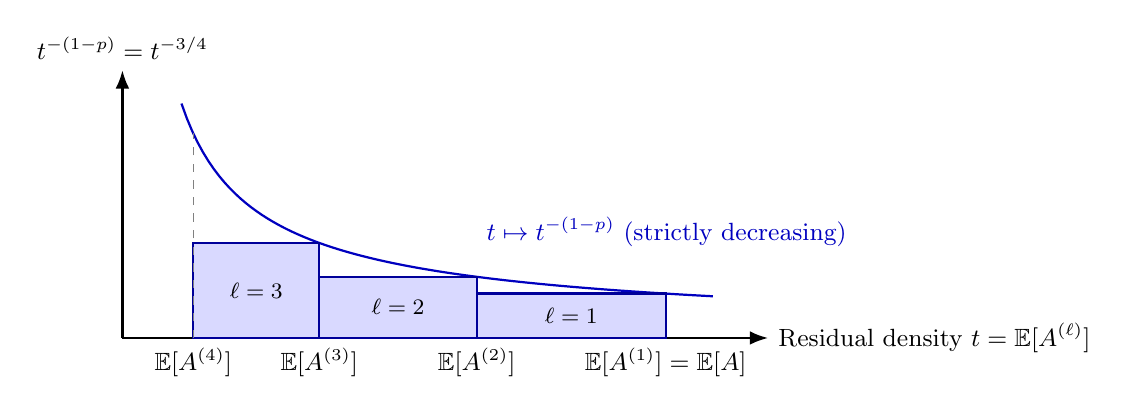
\begin{tikzpicture}[scale=1.0, >=Latex]
    % Axes
    \draw[->, thick] (0,0) -- (8.2,0) node[right] {\small Residual density $t = \dens{A^{(\ell)}}$};
    \draw[->, thick] (0,0) -- (0,3.4) node[above] {\small $t^{-(1-p)} = t^{-3/4}$};

    % Smooth curve y = 2.4 / x^{0.75} with exact exponent 0.75 = 3/4
    \draw[thick, blue!75!black, domain=0.75:7.5, samples=100] plot (\x, {2.4 / (\x)^0.75});
    \node[blue!75!black, right] at (4.5, 1.35) {\small $t \mapsto t^{-(1-p)}$ (strictly decreasing)};

    % Staircase rectangles under the curve (from right to left: A^(1) > A^(2) > A^(3) > A^(4))
    % Points: x4=0.9, x3=2.5, x2=4.5, x1=6.9
    % Heights at right endpoints x_l = E[A^(l)] along 2.4 / x^{0.75}:
    \fill[blue!15, draw=blue!60!black, thick] (0.9,0) rectangle (2.5, {2.4/(2.5^0.75)});
    \fill[blue!15, draw=blue!60!black, thick] (2.5,0) rectangle (4.5, {2.4/(4.5^0.75)});
    \fill[blue!15, draw=blue!60!black, thick] (4.5,0) rectangle (6.9, {2.4/(6.9^0.75)});

    % Dashed vertical lines and labels
    \draw[dashed, gray] (0.9,0) -- (0.9, {2.4/(0.9^0.75)});
    \node[below] at (0.9,0) {\small $\dens{A^{(4)}}$};
    \node[below] at (2.5,0) {\small $\dens{A^{(3)}}$};
    \node[below] at (4.5,0) {\small $\dens{A^{(2)}}$};
    \node[below] at (6.9,0) {\small $\dens{A^{(1)}} = \dens{A}$};

    % Annotation inside boxes
    \node at (5.7, 0.28) {\footnotesize $\ell = 1$};
    \node at (3.5, 0.39) {\footnotesize $\ell = 2$};
    \node at (1.7, 0.60) {\footnotesize $\ell = 3$};
\end{tikzpicture}
\caption{Riemann-sum telescoping (\Cref{lem:riemann}), drawn for $p = 1/4$. Since $\dens{A_\ell} \ge \dens{A^{(\ell)}}$ and $\Delta t_\ell := \dens{A^{(\ell)}} - \dens{A^{(\ell+1)}} = \frac{\abs{X_\ell}\abs{Y_\ell}}{\abs{X}\abs{Y}}\dens{A_\ell}$, the $\ell$-th extracted 2D rectangle contributes $\frac{\abs{X_\ell}\abs{Y_\ell}}{\abs{X}\abs{Y}}\dens{A_\ell}^p \le \big(\dens{A^{(\ell)}}\big)^{-(1-p)}\Delta t_\ell \le \int_{\dens{A^{(\ell+1)}}}^{\dens{A^{(\ell)}}} t^{-(1-p)}\,dt$. The shaded boxes thus form a lower Riemann sum under $t \mapsto t^{-(1-p)}$, which eliminates the $(d+2)$ blowup factor.}
\label{fig:riemann}
\end{figure}

\paragraph{The fractional potential.}
Instead of unweighted volume, we track the fractional density-weighted potential $\pot$ of \Cref{sec:overview-afklm}. Our inductive invariant (\Cref{lem:potential}) states that every call of \DecomposeThreeD{} at depth $h$ whose matrix $A$ has column degrees at most $2\alpha$ returns pieces with $\pot(\mathcal{S}) \le \Lambda_h \alpha^{1/4}\dens{B}^{1/4}\abs{X}\abs{Y}\abs{Z}$, where $\Lambda_h = 128 \cdot 2^h$. Why does raising the densities to the fractional power $p = 1/4 \in (0, 1/2)$ eliminate both $(d+2)$ factors? Two observations answer this; \Cref{rem:why-one-fourth} explains why our argument requires $p \in (0, 1/2)$.
\begin{itemize}[leftmargin=*]
    \item \emph{Riemann sum on $A$ in 2D (\Cref{lem:riemann}, \Cref{fig:riemann}).} As \DecomposeTwoD{} extracts edge-disjoint rectangles $A_1, \dots, A_{L-1}$ from $A$, the residual density decreases, $\dens{A^{(1)}} > \dens{A^{(2)}} > \cdots > \dens{A^{(L)}}$, with $\dens{A^{(\ell)}} - \dens{A^{(\ell+1)}} = \frac{\abs{X_\ell}\abs{Y_\ell}}{\abs{X}\abs{Y}}\dens{A_\ell}$ and $\dens{A_\ell} \ge \dens{A^{(\ell)}}$. Multiplying this identity by $\dens{A_\ell}^{-(1-p)} \le \big(\dens{A^{(\ell)}}\big)^{-(1-p)}$ bounds the $\ell$-th term by the area of a box lying underneath the decreasing curve $t \mapsto t^{-(1-p)}$ on $[\dens{A^{(\ell+1)}}, \dens{A^{(\ell)}}]$. Summing over $\ell$ telescopes the integrals to
    \[
        \sum_{\ell=1}^L \dens{A_\ell}^p\abs{X_\ell}\abs{Y_\ell} \le \frac{1}{p}\dens{A}^p\abs{X}\abs{Y} \qquad \left(= 4\dens{A}^{1/4}\abs{X}\abs{Y} \text{ for } p = \frac{1}{4}\right),
    \]
    with \emph{no} dependence on $d$.
    \item \emph{Concavity on $B$ in 3D (\Cref{lem:potential}).} Suppose \FindCube{} extracts a dense submatrix $B[Y^*, Z^*]$ of density $\beta^* = \dens{B[Y^*, Z^*]} \ge \beta := \dens{B}$ and area fraction $q = \frac{\abs{Y^*}\abs{Z^*}}{\abs{Y}\abs{Z}}$. The residual matrix $B - B[Y^*, Z^*]$ then has density $\delta = \beta(1 - q\frac{\beta^*}{\beta})$, and the concavity inequality $(1 - u)^{1/4} \le 1 - \frac{1}{4}u$ shows that the residual potential drops by at least
    \[
        \beta^{1/4} - \delta^{1/4} \ge \frac{1}{4}\left(\frac{\beta^*}{\beta}\right)^{3/4} q (\beta^*)^{1/4}.
    \]
    This drop contributes the negative term $-\frac{1}{4} W^*$ to the potential budget, where $W^* = \Lambda_h \alpha^{1/4}(\beta^*)^{1/4}\abs{X}\abs{Y^*}\abs{Z^*}$, and pays for all new pieces created in the current step. With $\gamma = \frac{1}{2048} = \Theta(1)$, the five-row budget of \Cref{tab:potential-budget} shows that the four positive contributions sum to at most $\frac{28}{256}W^*$, less than half of the potential drop $\frac{64}{256}W^*$.
\end{itemize}

\paragraph{Local cap normalization and column bucketing.}
When a subproblem restricts $X$ to $X_\ell \subsetneq X$, the column degrees of $A_\ell$ can vary across $y \in Y_\ell$, and some may exceed $2\dens{A_\ell}$. \Cref{lem:dyadic-bucketing} therefore partitions $Y_\ell$ into dyadic buckets $Y_{\ell, j}$ on which the column degrees of $A_\ell$ are capped by $2\alpha'_j = 2^{j+1}\dens{A_\ell}$. Markov's inequality bounds the fraction $p_j$ of columns in bucket $j$ by $2^{-j}$, and edge conservation ($\sum_j p_j\beta'_j = \dens{B'}$, where $\beta'_j$ is the density of the subproblem's matrix $B'$ on bucket $j$) then bounds the potential sum across all $D$ buckets by a universal geometric series, $\sum_{j \ge 0} 2^{-j/2} = \frac{1}{1 - 2^{-1/2}} < \frac{7}{2}$. Because the invariant is \emph{local}, normalized by each call's own column-degree cap $\alpha$, the child's cap $\alpha'_j = 2^j\dens{A_\ell}$ drops together with $\dens{A_\ell}$, at zero potential cost.

\subsection{Idea 4: Buying Depth with Density Jumps}
\label{sec:overview-depth}

In~\cite{AFKLM24}, per-level losses compound over the $O(d)$ levels of the outer recursion: $\log K = O(d\log M + d\log L)$ (Row~4 of \Cref{tab:bottlenecks}). This compounding would remain costly even after Ideas~1--3: if each of the $H = \Theta(d)$ levels of the 3D recursion could invoke a full 2D decomposition into $2^{\Theta(d^2)}$ rectangles while advancing by only $\Delta h = 1$ level, the total number of pieces would still be $(2^{\Theta(d^2)})^H = \exp(\Theta(d^3))$.

\begin{figure}[t]
\centering
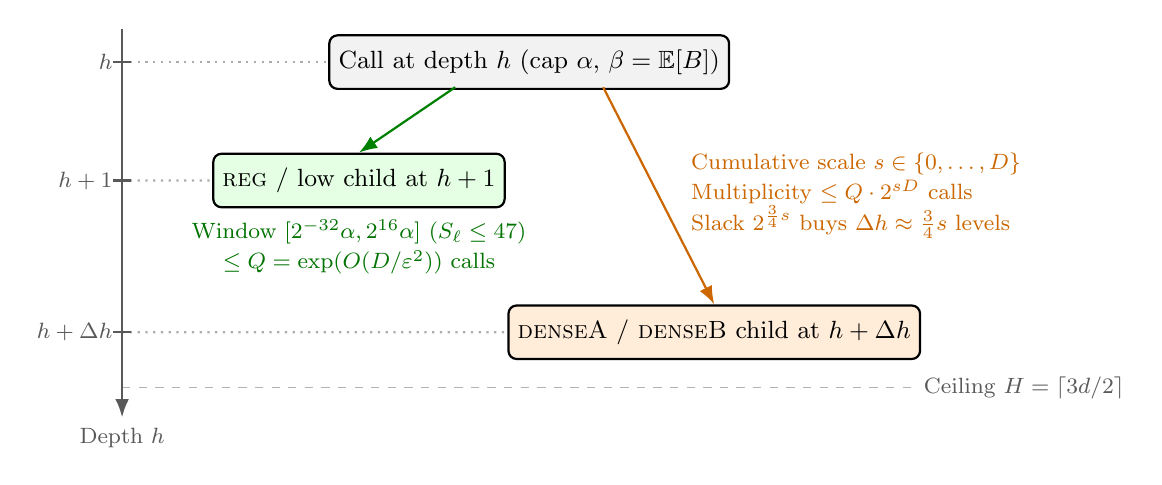
\begin{tikzpicture}[scale=0.94, >=Latex]
    % Root and child nodes
    \node[draw, rounded corners=3pt, fill=gray!10, thick, minimum width=4.4cm, minimum height=0.68cm] (root) at (0, 0) {\small Call at depth $h$ (cap $\alpha$, $\beta = \dens{B}$)};
    \node[draw, rounded corners=3pt, fill=green!10, thick, minimum width=3.6cm, minimum height=0.68cm] (norm) at (-2.3, -1.6) {\small \tagreg{} / low child at $h + 1$};
    \node[draw, rounded corners=3pt, fill=orange!15, thick, minimum width=4.0cm, minimum height=0.68cm] (jump) at (2.5, -3.65) {\small \tagdenseA{} / \tagdenseB{} child at $h + \Delta h$};

    % Horizontal depth guide lines
    \draw[dotted, gray!65, thick] (-5.5, 0) -- (root.west);
    \draw[dotted, gray!65, thick] (-5.5, -1.6) -- (norm.west);
    \draw[dotted, gray!65, thick] (-5.5, -3.65) -- (jump.west);
    \draw[dashed, gray!60] (-5.5, -4.4) -- (5.2, -4.4) node[right, gray!70!black] {\footnotesize Ceiling $H = \lceil 3d/2 \rceil$};

    % Depth axis on the far left
    \draw[->, thick, gray!70!black] (-5.5, 0.45) -- (-5.5, -4.8) node[below] {\footnotesize Depth $h$};
    \draw[thick, gray!70!black] (-5.62, 0) -- (-5.38, 0) node[left=3pt] {\footnotesize $h$};
    \draw[thick, gray!70!black] (-5.62, -1.6) -- (-5.38, -1.6) node[left=3pt] {\footnotesize $h + 1$};
    \draw[thick, gray!70!black] (-5.62, -3.65) -- (-5.38, -3.65) node[left=3pt] {\footnotesize $h + \Delta h$};

    % Left branch arrow and caption directly under the green node
    \draw[->, thick, green!50!black] (-1.0, -0.34) -- (norm.north);
    \node[text=green!45!black, align=center] at (-2.3, -2.5) {\footnotesize Window $[2^{-32}\alpha, 2^{16}\alpha]$ ($S_\ell \le 47$)\\[-1pt]\footnotesize $\le Q = \exp(O(D/\varepsilon^2))$ calls};

    % Right branch arrow and caption to the right of the orange arrow
    \draw[->, thick, orange!80!black] (1.0, -0.34) -- (jump.north) node[midway, right=8pt, text=orange!80!black, align=left] {\footnotesize Cumulative scale $s \in \{0, \dots, D\}$\\[-1pt]\footnotesize Multiplicity $\le Q \cdot 2^{s D}$ calls\\[-1pt]\footnotesize Slack $2^{\frac{3}{4}s}$ buys $\Delta h \approx \frac{3}{4}s$ levels};
\end{tikzpicture}
\caption{Buying recursion depth with density jumps (\Cref{sec:overview-depth,lem:recurrence}). Normal children stay within a constant density window ($S_\ell \le 47$, $S_B \le 4$); they incur no $2^{D^2}$ branching and advance by $\Delta h = 1$. Boosted children at cumulative dyadic scale $s$ (with $\beta^*/\beta \ge 2^s$ for $S_B = s$, or $\mu_\ell/\alpha \ge 2^{s-32}$ for $S_\ell = s$, where $\mu_\ell := \dens{A_\ell}$) spawn up to $Q 2^{s D}$ calls, but advance $\Delta h \approx \frac{3}{4}s$ levels ($\Delta_B(s)$ or $\Delta_A(s)$) deeper into the depth budget $H = \lceil 3d/2 \rceil$. Hence, along every root-to-leaf path of the recursion tree obtained by unrolling the same-depth $\mathcal{S}^*$ chains, the scales $s_i$ of the boosted, depth-increasing transitions satisfy $\sum s_i \le O(d)$ (with at most one final jump, of scale $s \le D$, reaching the ceiling $H$).}
\label{fig:depth-jumps}
\end{figure}

\paragraph{Constant-window capping and jump-adaptive depth (\Cref{fig:depth-jumps}).}
Our solution couples the inner 2D and 3D density increments to the outer recursion depth $h \in \{0, 1, \dots, H\}$, where $H := \lceil 3d/2 \rceil$. Searches whose density stays within a constant window are cheap, and a large density jump pays for itself by advancing the depth. (Recall $D = 2d$; the 3D decomposition runs the 2D tools with parameter $D$.)
\begin{enumerate}[leftmargin=*]
    \item \emph{Constant-window capping.} Inside \DecomposeTwoD{} and \FindCube{}, we confine the density of $A$ to the constant multiplicative window $[2^{-32}\alpha, 2^{16}\alpha]$ around the current column cap $\alpha$. \FindCube{} also caps the entry density of $B$ at $16\beta$, so any \tagnormal{} return satisfies $\beta^* < 16(1 + \frac{\varepsilon\gamma}{4})\beta < 17\beta$. We chose these powers of two so that the potential budget in \Cref{tab:potential-budget} closes. A rectangle or cube that stays inside its window has cumulative dyadic jump scale $S_\ell \le 47 = O(1)$ for $A$ and $S_B \le 4 = O(1)$ for $B$. Consequently, normal pieces suffer \emph{no} $2^{-D^2}$ shrinkage: their area loss and multiplicity per level are bounded by $Q = \exp(O(D/\varepsilon^2))$.
    \item \emph{Converting density jumps into depth.} Whenever a rectangle of $A$ or a cube of $B$ jumps above its cap at cumulative scale $s$, we halt the inner search and tag the result \tagdenseA{} or \tagdenseB{}. The potential weights density only by the exponent $\frac{1}{4}$, whereas edge conservation (for $A$) or concavity (for $B$) gains a factor linear in the density ratio. A $2^s$ density jump therefore creates a $2^{\frac{3}{4}s}$ potential slack. Since $\Lambda_h = 128 \cdot 2^h$ doubles with each level $h$, we can spend this slack to advance the child call directly by
    \[
        \Delta h = \min\!\Big(H - h, \, \max\big(1, \lfloor \tfrac{3}{4}s - O(1) \rfloor\big)\Big) \approx \frac{3}{4}s
    \]
    levels in a single step. The constant offsets are made explicit in $\Delta_B(s)$ and $\Delta_A(s)$ below.
\end{enumerate}

\paragraph{The master recurrence.}
Let $T(h)$ denote the maximum number of pieces returned by any valid call to \DecomposeThreeD{} at depth at least $h$. The piece bound of \Cref{lem:recurrence} follows in four steps.
\begin{enumerate}[label=(\roman*), leftmargin=*]
    \item \emph{Unrolling the $B$-loop.} Unrolling the tail recursion on $B - B[Y^*, Z^*]$ at depth $h < H$ yields the recurrence
    \begin{equation}\label{eq:overview-recurrence}
        T(h) \le 1 + Q + Q\,T(h + 1) + \sum_{s=0}^{D} Q\,2^{s D}\Big(T\big(h + \Delta_B(s)\big) + T\big(h + \Delta_A(s)\big)\Big),
    \end{equation}
    where $\log_2 Q = O(D/\varepsilon^2)$, $\Delta_B(s) = \min(H-h, \max(1, \lfloor \frac{3}{4}s - 2 \rfloor))$, and $\Delta_A(s) = \min(H-h, \max(1, \lfloor \frac{3}{4}s - 35 \rfloor))$. The term $Q\,T(h+1)$ accounts for the normal children (from \tagreg{} rectangles and the low-density remainder), and the sum for the boosted children at each scale $s$, at most $Q\,2^{sD}$ of each kind, even those that advance only one level.
    \item \emph{Ceiling base case.} At $h = H$, splitting $B$ into sparse pieces of density $\le 2^{-D}$ (or into one-edge pieces when $\abs{Y}\abs{Z} < 2^D$) produces at most $T(H) \le 3 \cdot 2^D$ pieces, with \emph{no} $2^{D^2}$ factor.
    \item \emph{Ceiling hits versus interior jumps.} Let $h < H$. A jump that reaches the ceiling, $h + \Delta h = H$, pays $2^{s D} T(H) \le 3 \cdot 2^{D + D^2}$, and this happens at most once along any root-to-leaf path. A jump to an interior level $h + \Delta h < H$ satisfies $s \le 50\Delta h$, so its multiplicity $2^{s D}$ is absorbed by the factor $2^{-50 D \Delta h}$ in the inductive bound $T(h + \Delta h) \le 3 \cdot 2^{D + D^2 + \Gamma(H - h - \Delta h)}$, where $\Gamma = 50 D + \lceil \log_2((2D+4)Q) \rceil = O(D/\varepsilon^2)$.
    \item \emph{Conclusion.} Downward induction from $h = H$ to $h = 0$ gives $T(0) \le 3 \cdot 2^{D + D^2 + \Gamma H} = \exp(O(d^2 / \varepsilon^2))$.
\end{enumerate}

\subsection{Putting It Together and the \texorpdfstring{$c = 2$}{c = 2} Barrier}
\label{sec:overview-together}

\TriangleDetect{} (\Cref{alg:triangle}) fixes $\varepsilon = 1/160$, so that $2^{-\varepsilon d / 2} = 2^{-d/320}$, and sets $d = \max(320, \lfloor c_0 \sqrt{\lfloor \log_2 n \rfloor} \rfloor)$, where $c_0 := 1/b_0$ for a sufficiently large integer $b_0 \ge 1$. By \Cref{thm:main-decomp}, \DecomposeThreeD{} runs in $n^2 \exp(O(d^2)) = O(n^{2.1})$ time and outputs $K \le \exp(O(d^2))$ pieces with $\pot(\mathcal{S}) \le 128 n^3$. Querying the pieces as in \Cref{sec:overview-afklm} then takes $n^2 2^{O(d^2)} + O(2^{-d/320} n^3) = O(n^3 / 2^{\Omega(\sqrt{\log n})})$ time. The Vassilevska Williams--Williams reduction (\Cref{lem:bmm-to-tridet}) transfers this bound to $n \times n$ BMM.

Finally, $\exp(\Omega(d^2))$ pieces and $2^{-\Omega(d^2)}$ single-step row loss are unavoidable for the sifting step used here and in~\cite{AFKLM24} (\Cref{prop:tightness}). As discussed in \Cref{sec:discussion}, this is a lower bound for that sifting-and-extraction routine, not for arbitrary grid-regularity decompositions or arbitrary combinatorial BMM algorithms. The construction partitions $X$ into $B = 2^{\lfloor d^2/2 \rfloor}$ equal row blocks $X_1, \dots, X_B$, and assigns each block $X_m$ a column subset $Y_m \subseteq Y$ of density $2^{1-d}$, with pairwise intersections $\abs{Y_m \cap Y_{m'}} \le (1 + \varepsilon/4)2^{2-2d}\abs{Y}$. Then $A$ has uniform row degree $2^{1-d} > 2^{-d}$. Yet on the neighborhood $Y_{x^*} = Y_m$ of any witness row $x^* \in X_m$, only the rows $x' \in X_m$, a $2^{-\lfloor d^2/2 \rfloor}$-fraction of $X$, have degree $\ge (1 + \varepsilon/2)2^{1-d}$. A single sifting step must therefore restrict $X$ to $X_m$, losing a factor of $2^{-\Omega(d^2)}$ in $\abs{X}$, and $\Omega(2^{d^2/2})$ blocks must be extracted before the residual density drops to $2^{-d}$.

\subsection{Organization and Procedure Call Graph}
\label{sec:overview-org}

\Cref{sec:prelim} sets up notation, grid norms, the regular-product theorem (\Cref{prop:regular-product}), minimum-degree pruning (\Cref{lem:min-degree}), and the two-stage sampler (\Cref{lem:two-stage-sampler}). \Cref{sec:2d} develops the 2D toolkit: \EstimateNorm{}, \Sift{}, \FindRect{}, \DecomposeTwoD{}, and the tightness construction. \Cref{sec:3d} presents the 3D decomposition and proves \Cref{thm:main-decomp}, and \Cref{sec:bmm} gives \TriangleDetect{} and proves \Cref{thm:main-bmm}. \Cref{sec:open} concludes with open problems, and \Cref{sec:ai-disclosure} contains our AI disclosure statement. The appendices prove the regular-product theorem and the two-stage sampler (\Cref{app:klm-proof,app:sampler}), discuss machine-model invariance (\Cref{app:models}), and verify the constants (\Cref{app:constants}). \Cref{tab:call-graph} summarizes the procedures of our algorithm and their call hierarchy.

\begin{table}[t]
\centering
\footnotesize
\setlength{\tabcolsep}{5pt}
\renewcommand{\arraystretch}{1.18}
\begin{tabularx}{\textwidth}{@{}>{\raggedright\arraybackslash}p{0.16\textwidth}>{\raggedright\arraybackslash}p{0.16\textwidth}>{\raggedright\arraybackslash}X>{\raggedright\arraybackslash}p{0.21\textwidth}@{}}
\toprule
\textbf{Procedure} & \textbf{Calls} & \textbf{Role} & \textbf{Analyzed In} \\
\midrule
$\TriangleDetect$ & $\DecomposeThreeD$ & Decomposes $(A, B)$ and queries each piece against $C$ & Alg.~\ref{alg:triangle}; Thm.~\ref{thm:main-bmm} \\
$\DecomposeThreeD$ & $\FindCube$,\newline $\DecomposeThreeD$ & Outer 3D recursion with jump-adaptive depth $h \le H$ & Alg.~\ref{alg:3d}; Lem.~\ref{lem:potential}, \ref{lem:recurrence} \\
$\FindCube$ & $\Prune$, $\Sift$,\newline $\DecomposeTwoD$,\newline $\FindCube$ & Extracts a regular or density-boosted 3D cube on $Y^* \times Z^*$ & Alg.~\ref{alg:3d}; Lem.~\ref{lem:cube-step} \\
$\DecomposeTwoD$ & $\FindRect$ & Capped 2D density-decrement loop on $A[X, Y']$ & Alg.~\ref{alg:2d}; Thm.~\ref{thm:2d-decomp}; Lem.~\ref{lem:riemann} \\
$\FindRect$ & $\Prune$, $\Sift$,\newline $\FindRect$ & Extracts one regular or $\tagdenseA$ rectangle & Alg.~\ref{alg:2d}; Lem.~\ref{lem:find-rect} \\
$\Sift$ & $\EstimateNorm$ & Dyadic $(2, d)$-biclique sifting across scales $s \in \{0, \dots, d-1\}$ & Alg.~\ref{alg:sift}; Lem.~\ref{lem:dyadic-sift} \\
$\EstimateNorm$ & Two-stage\newline sampler $\mathcal{T}$ & Exact $X$-average + sampled $Y$-average in $L_d(X \times \mathcal{T})$ & Alg.~\ref{alg:estimate-norm}; Lem.~\ref{lem:approx-grid-norm}, \ref{lem:two-stage-sampler} \\
$\Prune$ & --- & Greedy minimum-degree row/column pruning & Alg.~\ref{alg:prune}; Lem.~\ref{lem:min-degree} \\
\bottomrule
\end{tabularx}
\caption{Call graph of our procedures: for each procedure, the procedures it calls, its role, and where it is specified and analyzed.}
\label{tab:call-graph}
\end{table}

\section{Preliminaries}
\label{sec:prelim}

\subsection{Matrix Notation and Standing Conventions}
\label{sec:notation}

This subsection fixes the machine model and the notation used throughout the paper. \Cref{tab:notation} summarizes the notation, and \Cref{tab:constants} lists the fixed constants used in \Cref{sec:2d,sec:3d,sec:bmm}.

\paragraph{Machine model.}
We work in the standard Word RAM model with $O(\log n)$-bit words, using only $+, -, \times, \div$, comparisons, and array indexing (\Cref{app:models}). Externally supplied rational parameters such as $\varepsilon$ are assumed to have $O(\log n)$-bit numerators and denominators; longer external encodings contribute an additional factor polynomial in their length. Internally generated rationals need not have short encodings: for example, the exact sampler confidence $(\alpha'/2)^d$ used by \EstimateNorm{} may have numerator and denominator of $\Theta(d\log n)$ bits. We handle such rationals exactly with multiprecision integer arithmetic, and the analyses include its cost. Alternatively, the regularity and sampling parameters may be rounded down to dyadic rationals within a factor of $2$, with the corresponding constant-factor adjustment of the grid-norm parameter $d$ (\Cref{app:models}).

\begin{table}[t]
\centering
\footnotesize
\setlength{\tabcolsep}{3.5pt}
\begin{tabularx}{\textwidth}{@{}l>{\raggedright\arraybackslash}Xl@{}}
\toprule
\textbf{Symbol} & \textbf{Meaning} & \textbf{Formula / Reference} \\
\midrule
$\supp(A), \, \nnz(A)$ & Support and number of ones of $A \in \{0, 1\}^{X \times Y}$ & $\nnz(A) = \abs{\supp(A)}$ \\
$\dens{A}$ & Density of $A$ on $X \times Y$ & $\E_{(x, y) \in X \times Y}[A(x, y)] = \frac{\nnz(A)}{\abs{X}\abs{Y}}$ \\
$\deg_A(x), \, \deg_{A^T}(y)$ & Normalized row and column degrees & $\E_{y \in Y}[A(x, y)], \; \E_{x \in X}[A(x, y)]$ \\
$Y_x, \, A_x$ & Neighborhood of $x$ in $Y$ and restriction $A[X, Y_x]$ & $\abs{Y_x} = \deg_A(x)\abs{Y}$ \\
$A[X', Y']$ & Induced submatrix on $X' \times Y'$ (zero-extended in sums) & \Cref{sec:notation} \\
$AB, \, A \star B, \, A \circ B$ & Standard, Boolean, and normalized matrix products & $(A \circ B)(x, z) = \E_{y \in Y}[A(x, y)B(y, z)]$ \\
$\norm{A}_{U(k, \ell)}$ & $(k, \ell)$-grid norm of $A$ & \Cref{def:grid-norm}, \eqref{eq:grid-norm-def} \\
$(\varepsilon, k, \ell)$-regular & $\norm{A}_{U(k, \ell)} \le (1 + \varepsilon)\dens{A}$ & \Cref{def:grid-norm} \\
$\varepsilon$-min-degree & $\deg_A(x) \ge (1 - \varepsilon)\dens{A}$ for all $x \in X$ & \Cref{sec:notation} \\
$\pot(\mathcal{S})$ & Fractional density-weighted potential of an indexed list $\mathcal{S}$ of pieces & $\sum_{k=1}^K \dens{A_k}^{1/4}\dens{B_k}^{1/4}\abs{X_k}\abs{Y_k}\abs{Z_k}$ \\
$d, \, D = 2d$ & Grid-norm parameter ($d \ge 2/\varepsilon$) and even exponent $2d$ & \Cref{thm:main-decomp} \\
$h, \, H = \lceil 3d/2 \rceil$ & Current 3D recursion depth and the depth ceiling & \Cref{sec:3d} \\
$s, \, S_\ell, \, S_B$ & Single-step and cumulative dyadic density-jump scales ($\le D$) & \Cref{sec:2d,sec:3d} \\
\bottomrule
\end{tabularx}
\caption{Notation. The last column gives a defining formula or a reference.}
\label{tab:notation}
\end{table}

\begin{table}[t]
\centering
\footnotesize
\setlength{\tabcolsep}{3pt}
\begin{tabularx}{\textwidth}{@{}lll>{\raggedright\arraybackslash}Xl@{}}
\toprule
\textbf{Symbol} & \textbf{Value} & \textbf{Where Fixed} & \textbf{Constraint Enforced (see \Cref{tab:potential-budget})} & \textbf{Used In} \\
\midrule
$\varepsilon$ & $\le 1/160$ & \Cref{thm:main-decomp} & $80\varepsilon \le 1/2$ in \Cref{prop:regular-product} & \Cref{sec:bmm} \\
$\gamma$ & $1/2048$ & \Cref{sec:3d-alg} & $28\sqrt{2}\gamma < 40/2048 = 5/256$ (Row 4, \Cref{tab:potential-budget}) & \Cref{lem:potential} \\
$A$-window & $[2^{-32}\alpha, 2^{16}\alpha]$ & \Cref{sec:2d-decomp,sec:3d-alg} & $S_\ell \le 47$ on $\tagreg$; $(2^{-32})^{1/4} = 2^{-8}$ (Row 2) & \Cref{lem:potential} \\
$B$-window & $[\beta, 16\beta)$ (entry) & \Cref{sec:3d-alg} & Entry cap $< 16\beta \implies \beta^* < 17\beta, \, S_B \le 4$ on $\tagnormal$ & \Cref{lem:cube-step,lem:potential} \\
$\Lambda_h$ & $128 \cdot 2^h$ & \Cref{lem:potential} & $\Lambda_0 = 128 \implies 7/\Lambda_0 = 14/256$ (Row 1) & \Cref{lem:potential} \\
$H$ & $\lceil 3d/2 \rceil$ & \Cref{sec:3d-alg} & $\frac{3}{4}D = \frac{3}{2}d \le H \implies \Lambda_H \ge 4 \cdot 2^{3D/4}$ at $h = H$ & \Cref{clm:pot-base} \\
$\Delta h_B$ & $\lfloor \frac{3}{4}\log_2(\beta^*/\beta) - 2 \rfloor$ (raw) & \Cref{alg:3d} & On $\tagdenseB$ calls ($h < H$, $\beta^* \ge 16\beta$): $\Delta h_B \in [1, H-h]$, $2^{\Delta h_B} \le \frac{1}{4}(\beta^*/\beta)^{3/4}$ & \Cref{clm:pot-boost} \\
$\Delta h_\ell$ & $\lfloor \frac{3}{4}\log_2(\dens{A_\ell}/\alpha) - 11 \rfloor$ (raw) & \Cref{alg:3d} & On $\tagdenseA$ children ($h < H$, $\mu_\ell \ge 2^{16}\alpha$): $\Delta h_\ell \in [1, H-h]$, $2^{\Delta h_\ell}\mu_\ell^{1/4} \le 2^{-11}\alpha^{-3/4}\mu_\ell$ & \Cref{clm:pot-normal} \\
$M_{\text{rect}}$ & $\exp(O(D\varepsilon^{-1}\log(2/\varepsilon)))$ & \Cref{thm:2d-decomp} & Exact formula in \Cref{thm:2d-decomp} (2D non-dyadic shrinkage) & \Cref{lem:recurrence} \\
$M_{\text{cube}}$ & $\exp(O(d\varepsilon^{-2}))$ & \Cref{lem:cube-step} & Exact formula in \Cref{lem:cube-step} (3D non-dyadic shrinkage) & \Cref{lem:recurrence} \\
\bottomrule
\end{tabularx}
\caption{Constants and parameters fixed in the 2D and 3D decompositions (verified in \Cref{app:constants}). ``(raw)'' marks a depth increment before it is clamped to $[1, H - h]$ in \Cref{alg:3d}, and $\mu_\ell := \dens{A_\ell}$ (\Cref{line:3d-dhl}).}
\label{tab:constants}
\end{table}

\paragraph{Notation.}
Set $[0] := \emptyset$, and for an integer $k \ge 1$, write $[k] := \{1, \dots, k\}$. For a finite non-empty set $S$, $\E_{x \in S}$ and $\Pr_{x \in S}$ denote expectation and probability over a uniformly random $x \in S$. We view binary matrices $A \in \{0, 1\}^{X \times Y}$ on finite non-empty vertex sets $X, Y$ as bipartite graphs between $X$ and $Y$. Whenever a submatrix $A[X', Y']$ appears inside a matrix sum on $X \times Y$ (such as $A - A[X', Y']$ or $\sum_\ell A_\ell$), we identify $A[X', Y']$ with its zero-extension outside $X' \times Y'$. Finally, to state \Cref{prop:regular-product} we need the following notion: for $\alpha, \varepsilon, \delta \ge 0$, a matrix $M \in \R_{\ge 0}^{X \times Z}$ is \emph{$(\alpha, \varepsilon, \delta)$-uniform} if $\Pr_{(x, z) \in X \times Z}[(1 - \varepsilon)\alpha \le M(x, z) \le (1 + \varepsilon)\alpha] \ge 1 - \delta$.

\subsection{Grid Norms and Uniformity of Regular Products}
\label{sec:grid-norms}

We recall the $(k, \ell)$-grid norm of~\cite{KelleyLM23,AFKLM24} and grid regularity, which \Cref{def:pieces} requires of regular pieces. We then state the regular-product theorem, which the query phase (\Cref{sec:bmm}) uses to handle such pieces.

\begin{definition}[Grid norm and regularity]
\label{def:grid-norm}
For a matrix $A \in \R_{\ge 0}^{X \times Y}$ on finite non-empty sets $X, Y$ and integers $k, \ell \ge 1$, the \emph{$(k, \ell)$-grid norm} of $A$ is
\begin{equation}\label{eq:grid-norm-def}
    \norm{A}_{U(k, \ell)} := \left( \E_{\substack{x_1, \dots, x_k \in X \\ y_1, \dots, y_\ell \in Y}} \prod_{i=1}^k \prod_{j=1}^\ell A(x_i, y_j) \right)^{\frac{1}{k\ell}}.
\end{equation}
By Fubini's theorem,
\begin{equation}\label{eq:grid-norm-fubini}
    \norm{A}_{U(k, \ell)}^{k\ell} = \E_{x_1, \dots, x_k \in X} \left( \E_{y \in Y} \prod_{i=1}^k A(x_i, y) \right)^\ell = \E_{y_1, \dots, y_\ell \in Y} \left( \E_{x \in X} \prod_{j=1}^\ell A(x, y_j) \right)^k.
\end{equation}
More generally, for any real matrix $M \in \R^{X \times Y}$, any even integer $k \ge 2$, and any integer $\ell \ge 1$, the right-hand side of~\eqref{eq:grid-norm-fubini} is a non-negative average of even powers, defining $\norm{M}_{U(k, \ell)} \ge 0$. For $\varepsilon > 0$ and $A \in \R_{\ge 0}^{X \times Y}$, we say that $A$ is \emph{$(\varepsilon, k, \ell)$-regular} if $\norm{A}_{U(k, \ell)} \le (1 + \varepsilon)\dens{A}$.
\end{definition}

The structural foundation of grid regularity is the following theorem of Kelley, Lovett, and Meka~\cite[Lemma~4.8]{KelleyLM23}, restated in~\cite[Theorem~2.1]{AFKLM24}. We state its specialization to even integers $D = 2d \ge 4/\varepsilon$ and non-zero matrices, and give a complete proof in \Cref{app:klm-proof}.

\begin{proposition}[Uniformity of regular products]
\label{prop:regular-product}
Let $A \in \R_{\ge 0}^{X \times Y}$ and $B \in \R_{\ge 0}^{Y \times Z}$ be non-zero matrices on finite non-empty sets $X, Y, Z$, let $\varepsilon \in (0, 1/80)$, and let $D \ge 4/\varepsilon$ be an even integer. If $A$ and $B^T \in \R_{\ge 0}^{Z \times Y}$ are both $(\varepsilon, 2, D)$-regular and $\varepsilon$-min-degree, then $A \circ B$ is $(\dens{A}\dens{B}, \, 80\varepsilon, \, 2^{-\varepsilon D / 2})$-uniform on $X \times Z$. In particular, for $\varepsilon \le 1/160$, at least a $(1 - 2^{-\varepsilon D / 2})$-fraction of all pairs $(x, z) \in X \times Z$ satisfy
\[
    (A \circ B)(x, z) \ge \frac{1}{2}\dens{A}\dens{B} > 0.
\]
\end{proposition}

\subsection{Minimum-Degree Pruning and Oblivious Sampling}
\label{sec:prelim-tools}

This subsection presents two building blocks of our 2D and 3D algorithms. Minimum-degree pruning, used by \FindRect{} and \FindCube{} (\Cref{sec:2d-decomp,sec:3d-alg}), either certifies a min-degree condition or increases the density. A two-stage oblivious sampler lets \EstimateNorm{} (\Cref{sec:2d-norm}) replace inner averages over $Y$ by averages over short sample sequences.

\paragraph{Minimum-degree pruning.}
\Prune{} (\Cref{alg:prune}) is the greedy minimum-degree pruning procedure of~\cite[Algorithm~5.1 \& Lemma~5.1]{AFKLM24}. Starting from $U' = U$, it repeatedly removes a minimum-degree vertex $u \in U'$ of degree $\deg_{M[U', V]}(u) < (1 - \varepsilon_0)\dens{M[U', V]}$ until either $M[U', V]$ is $\varepsilon_0$-min-degree or at least a $\gamma_0$-fraction of $U$ has been removed. We state \Prune{} for the rows of a matrix $M \in \{0, 1\}^{U \times V}$; applied to a transpose, it prunes columns.

\begin{algorithm}[t]
\caption{$\Prune(U, V, M, \varepsilon_0, \gamma_0)$}\label{alg:prune}
\textbf{Input:} Finite non-empty sets $U, V$; binary matrix $M \in \{0, 1\}^{U \times V}$; parameters $\varepsilon_0 \in (0, 1)$, $\gamma_0 \in (0, 1/2]$.\\
\textbf{Output:} A non-empty subset $U' \subseteq U$ and a status flag (\emph{certified} or \emph{boosted}).
\begin{algsteps}
    \item Initialize $U' \gets U$.\label{line:prune-init}
    \item \textbf{while} there exists $u \in U'$ with $\deg_{M[U', V]}(u) < (1 - \varepsilon_0)\dens{M[U', V]}$ \textbf{do}\label{line:prune-while}
    \item \quad Remove a minimum-degree vertex $u$ from $U'$.\label{line:prune-remove}
    \item \quad \textbf{if} $\abs{U'} \le (1 - \gamma_0)\abs{U}$ \textbf{then return} $(U', \text{\emph{boosted}})$.\label{line:prune-boost}
    \item \textbf{return} $(U', \text{\emph{certified}})$.\label{line:prune-cert}
\end{algsteps}
\end{algorithm}

\begin{lemma}[Minimum-degree pruning]
\label{lem:min-degree}
Let $U, V$ be finite non-empty sets, let $M \in \{0, 1\}^{U \times V}$, and let $\varepsilon_0 \in (0, 1)$ and $\gamma_0 \in (0, 1/2]$. Then $\Prune(U, V, M, \varepsilon_0, \gamma_0)$ (\Cref{alg:prune}) runs in time $O(\abs{U}\abs{V})$ and returns a non-empty subset $U' \subseteq U$ with $\abs{U'} \ge \max(1, \lfloor (1 - \gamma_0)\abs{U} \rfloor) \ge \frac{1}{3}\abs{U}$ such that, writing $M' := M[U', V]$:
\begin{enumerate}[leftmargin=*]
    \item \textbf{If \Prune{} returns \emph{certified}:} $M'$ is $\varepsilon_0$-min-degree on $U'$, $\dens{M'} \ge \dens{M}$, $\abs{U \setminus U'} < \gamma_0\abs{U}$ (so $U' = U$ whenever $\abs{U} \le 1/\gamma_0$), and if $U \setminus U' \ne \emptyset$ then $\dens{M[U \setminus U', V]} < (1 - \varepsilon_0)\dens{M'}$.
    \item \textbf{If \Prune{} returns \emph{boosted}:} $\abs{U} \ge 2$, $\abs{U'} = \lfloor (1 - \gamma_0)\abs{U} \rfloor \ge \max(1, \frac{1}{3}\abs{U})$, $\abs{U \setminus U'} = \lceil \gamma_0\abs{U} \rceil \ge \gamma_0\abs{U}$, and $\dens{M'} \ge \frac{1}{1 - \gamma_0\varepsilon_0}\dens{M} \ge (1 + \gamma_0\varepsilon_0)\dens{M}$.
\end{enumerate}
\end{lemma}

\begin{proof}
Write $M_{\text{curr}} := M[U', V]$ for the current set $U'$. A vertex $u$ has degree $\E_{v \in V}[M(u, v)]$ in $M_{\text{curr}}$ regardless of $U'$, and $\dens{M_{\text{curr}}}$ is the average degree over $u \in U'$.

\emph{Non-emptiness.} Whenever $\abs{U'} = 1$ (say $U' = \{u_0\}$), $\deg_{M_{\text{curr}}}(u_0) = \dens{M_{\text{curr}}} \ge (1 - \varepsilon_0)\dens{M_{\text{curr}}}$, so the loop condition at \Cref{line:prune-while} is false. Hence $\abs{U'} \ge 1$ always holds.

\emph{Monotone density.} A vertex is removed only if it has minimum degree and some vertex violates the degree condition, so its degree is $< (1 - \varepsilon_0)\dens{M_{\text{curr}}}$, below the average. Hence every removal weakly increases $\dens{M_{\text{curr}}}$, and every removed vertex has degree $< (1 - \varepsilon_0)\dens{M'}$.

\emph{Certified output.} If \Cref{line:prune-cert} returns \emph{certified}, no $u \in U'$ violates the degree condition, so $M'$ is $\varepsilon_0$-min-degree on $U'$, and $\dens{M'} \ge \dens{M}$ by monotonicity. Since \Cref{line:prune-boost} never triggered, $\abs{U \setminus U'} < \gamma_0\abs{U}$, which forces $\abs{U \setminus U'} = 0$ when $\abs{U} \le 1/\gamma_0$. If $U \setminus U' \ne \emptyset$, then $\dens{M[U \setminus U', V]}$, the average degree of the removed vertices, is $< (1 - \varepsilon_0)\dens{M'}$.

\emph{Boosted output.} If \Cref{line:prune-boost} returns \emph{boosted}, it triggered for the first time upon removing a single vertex from a set of size $> (1 - \gamma_0)\abs{U}$. Hence $\abs{U} \ge 2$ and $\abs{U'} = \lfloor (1 - \gamma_0)\abs{U} \rfloor \ge \max(1, \frac{1}{3}\abs{U})$. Since $\abs{U \setminus U'} \ge \gamma_0\abs{U}$ and every removed vertex has degree $< (1 - \varepsilon_0)\dens{M'}$,
\[
    \dens{M} = \frac{\abs{U'}}{\abs{U}}\dens{M'} + \frac{\abs{U \setminus U'}}{\abs{U}}\dens{M[U \setminus U', V]} \le (1 - \gamma_0\varepsilon_0)\dens{M'}.
\]

\emph{Running time.} Since degrees do not change, bucket-sorting $U$ by row degree in $O(\abs{U}\abs{V})$ time maintains the minimum-degree vertex in $O(\abs{U}\abs{V})$ total time.
\end{proof}

\paragraph{Oblivious sampling.}
Recall that for a finite non-empty set $Y$ and $\varepsilon', \delta' \in (0, 1)$, an \emph{$(\varepsilon', \delta')$-oblivious sampler} $\mathcal{T}$ of $Y$ is an indexed family (multiset) of non-empty sample sequences $T \in Y^t$, in which repeated sequences are retained with multiplicity, such that for every function $g : Y \to [0, 1]$,
\begin{equation}\label{eq:oblivious-sampler}
    \Pr_{T \in \mathcal{T}}\!\left[\,\abs{\E_{y \in T}[g(y)] - \E_{y \in Y}[g(y)]} \le \varepsilon'\,\right] \ge 1 - \delta',
\end{equation}
where $\Pr_{T \in \mathcal{T}}$ and $\E_{T \in \mathcal{T}}$ are taken uniformly over the index set of $\mathcal{T}$, and $\E_{y \in T}[g(y)] := \frac{1}{\abs{T}}\sum_{i=1}^{\abs{T}} g(T(i))$ averages uniformly over the positions of $T$. Likewise, $T^d$ is the family of the $\abs{T}^d$ tuples $(T(i_1), \dots, T(i_d))$ indexed by $(i_1, \dots, i_d) \in [\abs{T}]^d$, and averages over $T^d$ are uniform over these indices.

Our two-stage sampler composes the Goldreich--Wigderson sampler~\cite{GoldreichW97}, as stated in~\cite[Lemma~4.4]{AFKLM24}, with a second stage obtained by applying Zuckerman's extractor-to-sampler reduction~\cite[Lemma~2.6 \& Proposition~2.7]{Zuckerman97} to the explicit Parvaresh--Vardy extractor of Guruswami, Umans, and Vadhan~\cite[Theorem~1.5 \& Theorem~5.12]{GUV09}. The composition keeps the family size linear in $\abs{Y}$, while the sequence length grows only polylogarithmically in $1/\delta'$; \EstimateNorm{} needs both properties (\Cref{sec:overview-norm}). We prove the following lemma in \Cref{app:sampler}.

\begin{restatable}[Two-stage sampler]{lemma}{lemtwostagesampler}\label{lem:two-stage-sampler}
Let $Y$ be a finite non-empty set and let $\varepsilon', \delta' \in (0, 1)$. There is a deterministic algorithm that, in time $\abs{Y} \cdot \poly((\varepsilon')^{-1}, (\delta')^{-1}, \log\abs{Y})$, constructs an $(\varepsilon', \delta')$-oblivious sampler $\mathcal{T}$ of $Y$ consisting of an indexed family of equal-length sample sequences $T \in Y^t$ satisfying
\begin{equation}\label{eq:two-stage-sampler}
    \abs{\mathcal{T}} \le \abs{Y} \cdot \poly\!\big((\varepsilon')^{-1}, \, (\delta')^{-1}\big), \qquad
    \abs{T} \le \poly\!\big((\varepsilon')^{-1}, \, \log(2/\delta')\big) \quad \forall T \in \mathcal{T}.
\end{equation}
\end{restatable}

\section{The Two-Dimensional Toolkit}
\label{sec:2d}

This section develops the 2D procedures of our algorithm, which the 3D decomposition (\Cref{sec:3d}) calls with parameter $D = 2d$: grid-norm estimation (\Cref{sec:2d-norm}), dyadic sifting (\Cref{sec:2d-sift}), and the rectangle search and 2D decomposition (\Cref{sec:2d-decomp}). \Cref{sec:2d-tightness} proves that $2^{-\Omega(d^2)}$ single-step row loss is unavoidable for our sifting step. Throughout this section, $X$ and $Y$ are finite non-empty vertex sets with $n := \abs{X} + \abs{Y}$, $A \in \{0, 1\}^{X \times Y}$ is a binary matrix, $\varepsilon \in (0, 1)$ is a regularity parameter, and $d \ge 2$ is an integer.

\subsection{Grid-Norm Estimation}
\label{sec:2d-norm}

To select its witness row, \Sift{} needs the grid norms $\norm{A_x}_{U(1, d)}$, where $A_x = A[X, Y_x]$ and $Y_x = \{y \in Y : A(x, y) = 1\}$ for $x \in X$ with $\deg_A(x) > 0$ (Idea~2, \Cref{sec:overview-norm}); by convention, $\deg_A(x)^d \norm{A_x}_{U(1, d)}^d := 0$ whenever $\deg_A(x) = 0$. \EstimateNorm{} (\Cref{alg:estimate-norm}) outputs exact rational approximations $V_x = v_x^d$ of $\norm{A_x}_{U(1, d)}^d$ and never takes $d$-th roots.

\begin{algorithm}[t]
\caption{$\EstimateNorm(X, Y, A, d, \alpha')$}\label{alg:estimate-norm}
\textbf{Input:} Finite non-empty sets $X, Y$; binary matrix $A \in \{0, 1\}^{X \times Y}$; integer $d \ge 1$; accuracy $\alpha' \in (0, 1)$.\\
\textbf{Output:} Rational values $V_x = v_x^d \ge 0$ for all $x \in X$ with $\deg_A(x) > 0$.
\begin{algsteps}
    \item Construct an $(\varepsilon', \delta')$-oblivious sampler $\mathcal{T}$ of $Y$ via \Cref{lem:two-stage-sampler} with $\varepsilon' := \alpha' / 2$ and $\delta' := (\alpha' / 2)^d$.\label{line:est-sampler}
    \item For each $T \in \mathcal{T}$ and $(y_1, \dots, y_d) \in T^d$, let $u_{T, y_1, \dots, y_d} := \E_{x' \in X}\big[\prod_{j=1}^d A(x', y_j)\big]$.\algcomment{Exact $X$-average}\label{line:est-u}
    \item For each $x \in X$ with $\deg_A(x) > 0$, let $U_x := \E_{T \in \mathcal{T}}\E_{(y_1, \dots, y_d) \in T^d}\big[u_{T, y_1, \dots, y_d}\prod_{j=1}^d A(x, y_j)\big]$ and $V_x := U_x / \deg_A(x)^d$.\label{line:est-v}
    \item \textbf{return} $\{V_x\}_{x \in X : \deg_A(x) > 0}$.\label{line:est-ret}
\end{algsteps}
\end{algorithm}

\begin{lemma}[Grid-norm estimation]
\label{lem:approx-grid-norm}
For any integer $d \ge 1$ (the standing assumption $d \ge 2$ is not needed here) and $\alpha' \in (0, 1)$, $\EstimateNorm(X, Y, A, d, \alpha')$ (\Cref{alg:estimate-norm}) runs in time $n^2 (d / \alpha')^{O(d)}$ and outputs non-negative rational values $V_x$ for all $x \in X$ with $\deg_A(x) > 0$ such that $v_x := V_x^{1/d}$ satisfies
\begin{equation}\label{eq:approx-grid-norm-err}
    \abs{v_x - \norm{A_x}_{U(1, d)}} \le \frac{\alpha'}{\deg_A(x)}.
\end{equation}
\end{lemma}

\begin{proof}
\emph{Reduction to the full column set.} Fix $x \in X$ with $\deg_A(x) > 0$, and define $A'_x \in \{0, 1\}^{X \times Y}$ by $A'_x(x', y) := A(x', y)A(x, y)$. Comparing averages over $Y$ and over $Y_x$ gives
\[
    \norm{A'_x}_{U(1, d)}^d = \E_{x' \in X}\!\left[\left(\frac{1}{\abs{Y}}\sum_{y \in Y_x} A(x', y)\right)^d\right] = \left(\frac{\abs{Y_x}}{\abs{Y}}\right)^d \norm{A_x}_{U(1, d)}^d = \deg_A(x)^d \norm{A_x}_{U(1, d)}^d,
\]
so $\norm{A'_x}_{U(1, d)} = \deg_A(x)\norm{A_x}_{U(1, d)}$.

\emph{Sampling error.} Equip $X \times \mathcal{T}$ with the uniform measure (over $x' \in X$ and the index set of $\mathcal{T}$), and define $a_x, b_x : X \times \mathcal{T} \to [0, 1]$ by
\[
    a_x(x', T) := \E_{y \in T}\big[A'_x(x', y)\big], \qquad b_x(x', T) := \E_{y \in Y}\big[A'_x(x', y)\big].
\]
By Fubini's theorem, $u_x := U_x^{1/d}$ at \Cref{line:est-v} equals $\norm{a_x}_{L_d(X \times \mathcal{T})}$; moreover, $\norm{b_x}_{L_d(X \times \mathcal{T})} = \norm{A'_x}_{U(1, d)}$. For each fixed $x' \in X$, the sampler guarantee~\eqref{eq:oblivious-sampler}, applied to $y \mapsto A'_x(x', y) \in [0, 1]$, gives $\abs{a_x(x', T) - b_x(x', T)} \le \varepsilon'$ for at least a $(1 - \delta')$-fraction of $T \in \mathcal{T}$. Since the difference is at most $1$ everywhere, $\E_{T \in \mathcal{T}}[\abs{a_x(x', T) - b_x(x', T)}^d] \le (\varepsilon')^d + \delta'$. Averaging over $x' \in X$ and applying Minkowski's reverse triangle inequality in $L_d(X \times \mathcal{T})$ together with $(u + v)^{1/d} \le u^{1/d} + v^{1/d}$ gives
\begin{align*}
    \abs{u_x - \norm{A'_x}_{U(1, d)}} &= \Big|\norm{a_x}_{L_d(X \times \mathcal{T})} - \norm{b_x}_{L_d(X \times \mathcal{T})}\Big| \le \norm{a_x - b_x}_{L_d(X \times \mathcal{T})} \\
    &\le \big((\varepsilon')^d + \delta'\big)^{1/d} \le \varepsilon' + (\delta')^{1/d} = \alpha'.
\end{align*}
Dividing by $\deg_A(x) > 0$ yields~\eqref{eq:approx-grid-norm-err}.

\emph{Running time.} Since $(\varepsilon')^{-1} = 2/\alpha'$ and $(\delta')^{-1} = (2/\alpha')^d$, we have $\log(2/\delta') = O(d\log(2/\alpha'))$. Hence \Cref{lem:two-stage-sampler} constructs $\mathcal{T}$ in time
\[
    \abs{Y}(2/\alpha')^{O(d)}\poly(\log(2\abs{Y})) \le O\!\left(n^2(d/\alpha')^{O(d)}\right),
\]
with $\abs{\mathcal{T}} \le \abs{Y}(2/\alpha')^{O(d)}$ and $\abs{T} \le \poly(d, (\alpha')^{-1})$, whence $\abs{T}^d \le (d/\alpha')^{O(d)}$. Each $u_{T, y_1, \dots, y_d}$ has denominator $\abs{X} \le n$, and each $U_x$ has denominator $\abs{X}\abs{\mathcal{T}}\abs{T}^d \le n^2(d/\alpha')^{O(d)}$. Thus each $V_x = U_x(\abs{Y}/\abs{Y_x})^d$ is an exact rational whose numerator and denominator in lowest terms have bit length $O(d(\log n + \log(d/\alpha')))$, that is, $O(d(1 + \frac{\log(d/\alpha')}{\log n}))$ machine words; this is $O(d)$ words whenever $\alpha' \ge n^{-O(1)}$ and $d \le n^{O(1)}$. Exact rational arithmetic and comparisons on such numbers take $\poly(d, \log(2/\alpha'))$ word operations, which are absorbed into $(d/\alpha')^{O(d)}$. In total, \Cref{alg:estimate-norm} takes time $(\abs{Y}\poly(\log(2\abs{Y})) + \abs{X}\abs{Y})(d/\alpha')^{O(d)} \le n^2(d/\alpha')^{O(d)}$.
\end{proof}

\subsection{Dyadic Sifting}
\label{sec:2d-sift}

\Sift{} (\Cref{alg:sift}), the density-increment step of the rectangle and cube searches (Idea~1, \Cref{sec:overview-sift}), either certifies that $A$ is $(\varepsilon, 2, d)$-regular or returns a denser sub-rectangle $(X', Y')$ at a dyadic scale $s \in \{0, 1, \dots, d-1\}$.

\begin{algorithm}[t]
\caption{$\Sift(X, Y, A, \varepsilon, d)$}\label{alg:sift}
\textbf{Input:} Finite non-empty sets $X, Y$; binary matrix $A \in \{0, 1\}^{X \times Y}$ with $\delta := (1 + \varepsilon/2)\dens{A} > 2^{-d}$; $\varepsilon \in (0, 1)$; integer $d \ge 2$.\\
\textbf{Output:} Either \tagreg{}, or a tuple $(X', Y', s)$ with $X' \subseteq X$, $Y' \subseteq Y$, and $s \in \{0, 1, \dots, d-1\}$.
\begin{algsteps}
    \item Let $\delta := (1 + \varepsilon/2)\dens{A}$, $\varepsilon_0 := \varepsilon/4$, and $\delta_s := 2^s\delta$ for $0 \le s \le d-1$.\label{line:sift-params}
    \item \textbf{for} $s = 0, 1, \dots, d-1$ \textbf{do}\algcomment{Outer dyadic row-degree check}\label{line:sift-outer-loop}
    \item \quad Let $X'_s := \{x \in X : \delta_s \le \deg_A(x) < 2\delta_s\}$. \textbf{if} $\abs{X'_s} \ge (\varepsilon/16)\, 2^{-(s+2)d}\abs{X}$ \textbf{then return} $(X'_s, Y, s)$.\label{line:sift-outer-ret}
    \item Let $X_{\ge \delta^2} := \{x \in X : \deg_A(x) \ge \delta^2\}$. \textbf{if} $X_{\ge \delta^2} = \emptyset$ \textbf{then return} \tagreg{}.\algcomment{Witness-row selection}\label{line:sift-xdelta2}
    \item Compute $\{V_x\} \gets \EstimateNorm(X, Y, A, d, \alpha')$ with $\alpha' := (\varepsilon_0 \delta^3)/8 = (\varepsilon \delta^3)/32$.\label{line:sift-est}
    \item Pick $x^* \in X_{\ge \delta^2}$ maximizing $V_{x^*}$, and let $Y' := Y_{x^*}$ and $A_{x^*} := A[X, Y']$.\label{line:sift-witness}
    \item \textbf{for} $s = 0, 1, \dots, d-1$ \textbf{do}\algcomment{Inner dyadic row-degree check}\label{line:sift-inner-loop}
    \item \quad Let $X'_{x^*, s} := \{x' \in X : \delta_s \le \deg_{A_{x^*}}(x') < 2\delta_s\}$. \textbf{if} $\abs{X'_{x^*, s}} \ge (\varepsilon/16)\, 2^{-(s+2)d}\abs{X}$ \textbf{then return} $(X'_{x^*, s}, Y', s)$.\label{line:sift-inner-ret}
    \item \textbf{return} \tagreg{}.\label{line:sift-reg}
\end{algsteps}
\end{algorithm}

\begin{lemma}[Dyadic sifting]
\label{lem:dyadic-sift}
Suppose $\delta := (1 + \frac{\varepsilon}{2})\dens{A} > 2^{-d}$ (which holds in particular whenever $\dens{A} \ge 2^{-d}$). Then $\Sift(X, Y, A, \varepsilon, d)$ (\Cref{alg:sift}) runs in time $n^2 \exp(O(d^2 + d\log(2/\varepsilon)))$, and:
\begin{enumerate}[leftmargin=*]
    \item If it returns $(X', Y', s)$, then $0 \le s \le d-1$ (indeed $2^s\delta \le \dens{A[X', Y']} \le 1$), and
    \begin{equation}\label{eq:dyadic-sift-guarantees}
        \dens{A[X', Y']} \ge 2^s\Big(1 + \frac{\varepsilon}{2}\Big)\dens{A}, \;\;
        \abs{X'} \ge \frac{\varepsilon}{16} 2^{-(s+2)d}\abs{X}, \;\;
        \abs{Y'} \ge \Big(1 + \frac{\varepsilon}{2}\Big)^2\dens{A}^2 \abs{Y} > 2^{-2d}\abs{Y}.
    \end{equation}
    \item If it returns \tagreg{}, then $A$ is $(\varepsilon, 2, d)$-regular.
\end{enumerate}
\end{lemma}

\begin{proof}
Set $\mu := \dens{A}$. Since $\delta = (1 + \frac{\varepsilon}{2})\mu > 2^{-d}$, we have $2^d\delta > 1$, so the dyadic slices $B_s := \{x \in X : \delta_s \le \deg_A(x) < 2\delta_s\}$ ($0 \le s \le d-1$) cover $\{x \in X : \deg_A(x) \ge \delta\}$.

\emph{Part~(1).} If \Cref{alg:sift} returns at \Cref{line:sift-outer-ret} or \Cref{line:sift-inner-ret}, every row in the returned set $X'$ has degree at least $\delta_s = 2^s(1 + \frac{\varepsilon}{2})\mu$ on $Y'$ and at most $1$, so $2^s\delta \le \dens{A[X', Y']} \le 1$. The return condition gives $\abs{X'} \ge \frac{\varepsilon}{16} 2^{-(s+2)d}\abs{X}$. Finally, either $Y' = Y$ (and then $\delta \le 2^{-s} \le 1$), or $\abs{Y'} = \deg_A(x^*)\abs{Y} \ge \delta^2\abs{Y} > 2^{-2d}\abs{Y}$ because $x^* \in X_{\ge \delta^2}$.

\emph{Part~(2).} Suppose that $\norm{A}_{U(2, d)} > (1 + \varepsilon)\mu$; we show that one of the two dyadic checks succeeds. Since $(1 + \varepsilon_0)\delta = (1 + \frac{\varepsilon}{4})(1 + \frac{\varepsilon}{2})\mu < (1 + \varepsilon)\mu$ and $\norm{A}_{U(2, d)} \le 1$, we have $1 \ge \norm{A}_{U(2, d)} > (1 + \varepsilon_0)\delta > \delta$, which forces $\delta < 1$ (so $\delta^2 < \delta$). By Fubini's theorem (\eqref{eq:grid-norm-fubini}; see also~\eqref{eq:overview-u2d} in \Cref{sec:overview-sift}), $\norm{A}_{U(2, d)}^{2d} = \E_{x \in X}[\deg_A(x)^d \norm{A_x}_{U(1, d)}^d]$, where rows with $\deg_A(x) = 0$ contribute $0$.
\begin{itemize}[leftmargin=*]
    \item \emph{Case A: No $x \in X_{\ge \delta^2}$ satisfies $\norm{A_x}_{U(1, d)} \ge (1 + \varepsilon_0)\delta$.}
    Partition $X$ into $X_{<\delta^2}$, $X_{[\delta^2, \delta)}$, and the $d$ dyadic slices $B_s = X'_s$ ($0 \le s \le d-1$). On $X_{<\delta^2} \cup X_{[\delta^2, \delta)}$, $\deg_A(x)^d \norm{A_x}_{U(1, d)}^d < (1 + \varepsilon_0)^d\delta^{2d}$, while on each $B_s \subseteq X_{\ge \delta^2}$, $\deg_A(x)^d\norm{A_x}_{U(1, d)}^d < (2^{s+1}\delta)^d(2\delta)^d = 2^{(s+2)d}\delta^{2d}$. Averaging over $x \in X$ gives
    \[
        (1 + \varepsilon_0)^{2d}\delta^{2d} < \norm{A}_{U(2, d)}^{2d} < (1 + \varepsilon_0)^d\delta^{2d} + \sum_{s=0}^{d-1} \frac{\abs{B_s}}{\abs{X}} 2^{(s+2)d}\delta^{2d}.
    \]
    Since $(1 + \varepsilon_0)^{2d} - (1 + \varepsilon_0)^d > d\varepsilon_0$, some $s \le d-1$ satisfies $\frac{\abs{B_s}}{\abs{X}} 2^{(s+2)d} > \varepsilon_0 = \frac{\varepsilon}{4}$. Then $\abs{X'_s} = \abs{B_s} > \frac{\varepsilon}{4} 2^{-(s+2)d}\abs{X} \ge \frac{\varepsilon}{16} 2^{-(s+2)d}\abs{X}$, so \Cref{line:sift-outer-ret} returns a sub-rectangle (at scale $s$ or earlier).
    \item \emph{Case B: Some $x_{\text{wit}} \in X_{\ge \delta^2}$ satisfies $\norm{A_{x_{\text{wit}}}}_{U(1, d)} \ge (1 + \varepsilon_0)\delta$, and \Cref{line:sift-outer-ret} did not return.}
    Then $X_{\ge \delta^2} \ne \emptyset$. By \Cref{lem:approx-grid-norm} with $\alpha' = \frac{\varepsilon_0\delta^3}{8}$, every $x \in X_{\ge \delta^2}$ satisfies $\abs{v_x - \norm{A_x}_{U(1, d)}} \le \frac{\alpha'}{\delta^2} = \frac{\varepsilon_0\delta}{8}$. Hence the maximizer $x^* \in X_{\ge \delta^2}$ of $V_x = v_x^d$ at \Cref{line:sift-witness} satisfies
    \[
        \norm{A_{x^*}}_{U(1, d)} \ge v_{x^*} - \frac{\varepsilon_0\delta}{8} \ge v_{x_{\text{wit}}} - \frac{\varepsilon_0\delta}{8} \ge \norm{A_{x_{\text{wit}}}}_{U(1, d)} - \frac{\varepsilon_0\delta}{4} \ge \left(1 + \frac{3}{4}\varepsilon_0\right)\delta.
    \]
    Partitioning $X$ into $D_{<\delta} := \{x' \in X : \deg_{A_{x^*}}(x') < \delta\}$ and the slices $D_s := X'_{x^*, s}$ ($0 \le s \le d-1$) gives $(1 + \frac{3}{4}\varepsilon_0)^d\delta^d \le \norm{A_{x^*}}_{U(1, d)}^d < \delta^d + \sum_{s=0}^{d-1} \frac{\abs{D_s}}{\abs{X}} 2^{(s+1)d}\delta^d$.
    Since $(1 + \frac{3}{4}\varepsilon_0)^d - 1 > \frac{3}{4}d\varepsilon_0$, some $s \le d-1$ satisfies $\abs{X'_{x^*, s}} = \abs{D_s} > \frac{3\varepsilon_0}{4} 2^{-(s+1)d}\abs{X} = \frac{3\varepsilon}{16} 2^{-(s+1)d}\abs{X} \ge \frac{\varepsilon}{16} 2^{-(s+2)d}\abs{X}$, so \Cref{line:sift-inner-ret} returns a sub-rectangle (at scale $s$ or earlier).
\end{itemize}

\emph{Running time.} Since $\alpha' = \frac{\varepsilon\delta^3}{32} \ge \frac{\varepsilon}{32} 2^{-3d}$, \Cref{lem:approx-grid-norm} bounds the time of \Cref{line:sift-est} by $n^2 (d/\alpha')^{O(d)} = n^2 \exp(O(d^2 + d\log(2/\varepsilon)))$.
\end{proof}

\subsection{Capped Rectangle Decomposition}
\label{sec:2d-decomp}

We now combine \Prune{} and \Sift{} into the rectangle search \FindRect{} and the 2D decomposition \DecomposeTwoD{} (\Cref{alg:2d}). A search stops at a regular rectangle or once the density reaches the cap $\alpha_{\text{cap}}$ (tag \tagdenseA{}), and the decomposition stops once the residual density is at most $\max(2^{-D}, \alpha_{\text{low}})$. The 3D decomposition uses the window $[\alpha_{\text{low}}, \alpha_{\text{cap}}] = [2^{-32}\alpha, 2^{16}\alpha]$ around its column cap $\alpha$ (constant-window capping, \Cref{sec:overview-depth}); the uncapped decomposition is a special case (\Cref{cor:uncapped-2d}).

\begin{algorithm}[t]
\caption{$\FindRect(X, Y, A, \varepsilon, D, \alpha_{\text{cap}})$ and $\DecomposeTwoD(X, Y, A, \varepsilon, D, \alpha_{\text{low}}, \alpha_{\text{cap}})$}\label{alg:2d}
\textbf{Procedure $\FindRect(X, Y, A, \varepsilon, D, \alpha_{\text{cap}})$:}\\
\textbf{Requires:} $\dens{A} \ge 2^{-D}$.
\begin{algsteps}
    \item \textbf{if} $\dens{A} \ge \alpha_{\text{cap}}$ \textbf{then return} $(X, Y, \tagdenseA)$.\label{line:findrect-cap1}
    \item Let $(X', \text{status}) \gets \Prune(X, Y, A, \varepsilon, 1/2)$ and $A' := A[X', Y]$.\label{line:findrect-prune}
    \item \textbf{if} $\text{status} = \text{\emph{boosted}}$ (or $\dens{A'} \ge (1 + \varepsilon/2)\dens{A}$) \textbf{then}\\
    \quad \textbf{return} $\FindRect(X', Y, A', \varepsilon, D, \alpha_{\text{cap}})$.\label{line:findrect-rec1}
    \item \textbf{if} $\dens{A'} \ge \alpha_{\text{cap}}$ \textbf{then return} $(X', Y, \tagdenseA)$.\label{line:findrect-cap2}
    \item \textbf{if} $\Sift(X', Y, A', \varepsilon, D)$ returns a sub-rectangle $(X'', Y'', s)$ \textbf{then}\\
    \quad \textbf{return} $\FindRect(X'', Y'', A[X'', Y''], \varepsilon, D, \alpha_{\text{cap}})$.\label{line:findrect-sift}
    \item \textbf{return} $(X', Y, \tagreg)$.\label{line:findrect-reg}
\end{algsteps}
\vspace{4pt}
\textbf{Procedure $\DecomposeTwoD(X, Y, A, \varepsilon, D, \alpha_{\text{low}}, \alpha_{\text{cap}})$:}
\begin{algsteps}[resume]
    \item Initialize $\ell \gets 1$, $A^{(1)} \gets A$, and $\tau_{\text{low}} := \max(2^{-D}, \alpha_{\text{low}})$.\label{line:dec2d-init}
    \item \textbf{while} $\dens{A^{(\ell)}} > \tau_{\text{low}}$ \textbf{do}\label{line:dec2d-while}
    \item \quad Let $(X_\ell, Y_\ell, \text{status}_\ell) \gets \FindRect(X, Y, A^{(\ell)}, \varepsilon, D, \alpha_{\text{cap}})$ and $A_\ell := A^{(\ell)}[X_\ell, Y_\ell]$.\label{line:dec2d-call}
    \item \quad Set $A^{(\ell+1)} \gets A^{(\ell)} - A_\ell$ and $\ell \gets \ell + 1$.\label{line:dec2d-sub}
    \item Set $L \gets \ell$, $(X_L, Y_L, A_L, \text{status}_L) \gets (X, Y, A^{(L)}, \tagsparse)$, and \textbf{return} the indexed list $\{(X_\ell, Y_\ell, A_\ell, \text{status}_\ell)\}_{\ell=1}^L$.\label{line:dec2d-ret}
\end{algsteps}
\end{algorithm}

\begin{lemma}[Rectangle search]
\label{lem:find-rect}
Let $D \ge 2$ be an integer, let $0 < \alpha_{\text{low}} < \alpha_{\text{cap}}$, and let $\tau_{\text{low}} := \max(2^{-D}, \alpha_{\text{low}})$ and $W := \alpha_{\text{cap}} / \tau_{\text{low}}$. Whenever $\dens{A^{(\ell)}} > \tau_{\text{low}}$, $\FindRect(X, Y, A^{(\ell)}, \varepsilon, D, \alpha_{\text{cap}})$ executes at most $r \le \min\!\big(\frac{2D}{\varepsilon}, \, 1 + \frac{2\log_2 \max(1, W)}{\varepsilon}\big)$ recursive steps whose dyadic scales $s_1, \dots, s_r \ge 0$ have sum $S_\ell := \sum_{t=1}^r s_t \in \{0, 1, \dots, D\}$ satisfying
\begin{equation}\label{eq:capped-goodrect-shrinkage}
    \dens{A_\ell} \ge 2^{S_\ell}\dens{A^{(\ell)}}, \qquad
    \abs{X_\ell} \ge \frac{1}{3}\left(\frac{\varepsilon}{48} 2^{-2D}\right)^r 2^{-S_\ell D}\abs{X}, \qquad
    \abs{Y_\ell} \ge 2^{-2Dr}\abs{Y}.
\end{equation}
If $\text{status}_\ell = \tagreg$, then $A_\ell$ is $(\varepsilon, 2, D)$-regular and $\varepsilon$-min-degree with $\dens{A^{(\ell)}} \le \dens{A_\ell} < \alpha_{\text{cap}}$; if $\text{status}_\ell = \tagdenseA$, then $\dens{A_\ell} \ge \max(\alpha_{\text{cap}}, 2^{S_\ell}\dens{A^{(\ell)}})$.
\end{lemma}

\begin{proof}
Write $(X_0, Y_0, A_0) := (X, Y, A^{(\ell)})$, and let $r$ be the number of recursive calls made by \FindRect{}. The density grows by a factor of at least $1 + \frac{\varepsilon}{2}$ per recursive step and stays in $(2^{-D}, 1]$, which bounds $r$ and $S_\ell$. If $r = 0$, the procedure either returns at \Cref{line:findrect-cap1}, or performs one certified pruning and returns at \Cref{line:findrect-cap2,line:findrect-reg}. In either case, $S_\ell = 0$, the density does not decrease ($\dens{A_\ell} \ge \dens{A_0}$), $\abs{X_\ell} \ge \frac{1}{3}\abs{X}$, and $Y_\ell = Y$. Thus both the step bound $r = 0 \le \min(\frac{2D}{\varepsilon}, 1 + \frac{2\log_2 \max(1, W)}{\varepsilon})$ and~\eqref{eq:capped-goodrect-shrinkage} hold.

\emph{Recursive steps.} Henceforth assume $r \ge 1$. Then $\dens{A_0} < \alpha_{\text{cap}}$, since \Cref{line:findrect-cap1} did not halt, so $W = \alpha_{\text{cap}}/\tau_{\text{low}} > \dens{A_0}/\tau_{\text{low}} > 1$ and $\max(1, W) = W$. Let $t \in \{1, \dots, r\}$ index the recursive steps before halting at $(X_r, Y_r, A_r)$; set $s_t := 0$ if step $t$ recurses at \Cref{line:findrect-rec1}, and let $s_t \ge 0$ be the scale returned by \Sift{} if it recurses at \Cref{line:findrect-sift}. In each step $t$, $\dens{A_{t-1}} < \alpha_{\text{cap}}$, and \Cref{lem:min-degree} (with $\gamma_0\varepsilon_0 = \varepsilon/2$ and $\abs{X'_{t-1}} \ge \frac{1}{3}\abs{X_{t-1}}$) and \Cref{lem:dyadic-sift}(1) give
\[
    \dens{A_t} \ge 2^{s_t}\left(1 + \frac{\varepsilon}{2}\right)\dens{A_{t-1}}, \qquad
    \abs{X_t} \ge \frac{\varepsilon}{48} 2^{-(s_t+2)D}\abs{X_{t-1}}, \qquad
    \abs{Y_t} \ge 2^{-2D}\abs{Y_{t-1}}.
\]

\emph{The halting call.} This call either returns $(X_r, Y_r, \tagdenseA)$ at \Cref{line:findrect-cap1}, or runs \Prune{} at \Cref{line:findrect-prune} in the \emph{certified} case (so $\dens{A'_r} \ge \dens{A_r}$ and $\abs{X'_r} \ge \frac{1}{3}\abs{X_r}$) and returns at \Cref{line:findrect-cap2} or \Cref{line:findrect-reg}. Thus
\[
    1 \ge \dens{A_\ell} \ge 2^{S_\ell}\left(1 + \frac{\varepsilon}{2}\right)^r \dens{A_0} > 2^{S_\ell}\left(1 + \frac{\varepsilon}{2}\right)^r 2^{-D},
\]
which implies $S_\ell \le D$ and $(1 + \frac{\varepsilon}{2})^r \le 2^D \implies r \le \frac{2D}{\varepsilon}$ (since $\log_2(1 + \frac{\varepsilon}{2}) \ge \frac{\varepsilon}{2}$ for $\varepsilon \in (0, 1)$). Likewise, since $\dens{A_{r-1}} < \alpha_{\text{cap}}$ and $\dens{A_0} > \tau_{\text{low}}$, we have $(1 + \frac{\varepsilon}{2})^{r-1} < \frac{\alpha_{\text{cap}}}{\tau_{\text{low}}} = W = \max(1, W) \implies r \le 1 + \frac{2\log_2 \max(1, W)}{\varepsilon}$. Multiplying the per-step shrinkage factors proves~\eqref{eq:capped-goodrect-shrinkage}; together with the return conditions, \Cref{lem:min-degree}(1), and \Cref{lem:dyadic-sift}(2), this gives the claims about $\text{status}_\ell$.
\end{proof}

\begin{theorem}[Capped 2D decomposition]
\label{thm:2d-decomp}
Let $D \ge 2$ be an integer, suppose $\alpha_{\text{low}} = 2^{-32}\alpha$ and $\alpha_{\text{cap}} = 2^{16}\alpha$ for some $\alpha > 0$ (so $\alpha_{\text{cap}}/\alpha_{\text{low}} = 2^{48}$), and let $M_{\text{rect}} := 3\big(\frac{48}{\varepsilon} 2^{2D}\big)^{97/\varepsilon} 2^{194D/\varepsilon} = \exp(O(D\varepsilon^{-1}\log(2/\varepsilon)))$ (\Cref{tab:constants}). Then $\DecomposeTwoD(X, Y, A, \varepsilon, D, \alpha_{\text{low}}, \alpha_{\text{cap}})$ (\Cref{alg:2d}) runs in time $n^2 \exp(O(D^2 + D\varepsilon^{-1}\log(2/\varepsilon)))$ and computes a decomposition $A = \sum_{\ell=1}^L A_\ell$ into an indexed list of $L \le 1 + 2^D M_{\text{rect}} 2^{D^2}$ edge-disjoint rectangles satisfying:
\begin{enumerate}[leftmargin=*]
    \item For every $\ell \in [L-1]$, $\abs{X_\ell}\abs{Y_\ell} \ge M_{\text{rect}}^{-1} 2^{-S_\ell D}\abs{X}\abs{Y}$ and $\abs{Y_\ell} \ge 2^{-194D/\varepsilon}\abs{Y}$; for each scale $s \in \{0, 1, \dots, D\}$, the number of rectangles $\ell \in [L-1]$ with $S_\ell = s$ is at most $L_s \le 2^D M_{\text{rect}} 2^{s D}$.
    \item Every $\ell \in [L-1]$ with $\text{status}_\ell = \tagreg$ is $(\varepsilon, 2, D)$-regular and $\varepsilon$-min-degree with $\tau_{\text{low}} < \dens{A_\ell} < \alpha_{\text{cap}}$ and $S_\ell \le 47$, and the total number of $\tagreg$ rectangles is at most $L_{\text{reg}} \le \sum_{s=0}^{\min(47, D)} L_s \le 48 \cdot 2^{48D} M_{\text{rect}} = \exp(O(D\varepsilon^{-1}\log(2/\varepsilon)))$.
    \item Every $\ell \in [L-1]$ with $\text{status}_\ell = \tagdenseA$ satisfies $\dens{A_\ell} \ge \max(2^{16}\alpha, 2^{S_\ell - 32}\alpha)$, and $\sum_{\ell : \text{status}_\ell = \tagdenseA} \dens{A_\ell}\abs{X_\ell}\abs{Y_\ell} \le \dens{A}\abs{X}\abs{Y}$.
    \item Rectangle $\ell = L$ has $X_L = X, Y_L = Y$ and $\dens{A_L} \le \tau_{\text{low}} = \max(2^{-D}, 2^{-32}\alpha)$.
\end{enumerate}
\end{theorem}

\begin{proof}
Since $W \le \alpha_{\text{cap}}/\alpha_{\text{low}} = 2^{48}$, \Cref{lem:find-rect} gives $r \le 1 + \frac{96}{\varepsilon} \le \frac{97}{\varepsilon}$, and hence $\abs{X_\ell}\abs{Y_\ell} \ge M_{\text{rect}}^{-1} 2^{-S_\ell D}\abs{X}\abs{Y}$. Any $\tagreg$ rectangle satisfies $2^{16}\alpha > \dens{A_\ell} > 2^{S_\ell}\tau_{\text{low}} \ge 2^{S_\ell - 32}\alpha$, so $S_\ell \le \min(47, D)$. Each rectangle $\ell \in [L-1]$ with $S_\ell = s$ has $\dens{A_\ell} > 2^{s-D}$ and therefore removes at least $\frac{\abs{X_\ell}\abs{Y_\ell}}{\abs{X}\abs{Y}}\dens{A_\ell} \ge 2^{-D} M_{\text{rect}}^{-1} 2^{-s D}$ from $\dens{A^{(\ell)}}$; as $\dens{A} \le 1$, this bounds $L_s \le 2^D M_{\text{rect}} 2^{s D}$. Since $s \le D$, every extracted rectangle removes at least $2^{-D} M_{\text{rect}}^{-1} 2^{-D^2}$ from the density, so $L - 1 \le 2^D M_{\text{rect}} 2^{D^2}$. The other claims follow from these bounds, \Cref{lem:find-rect}, edge-disjointness, and the \textbf{while} condition. Finally, there are at most $(L-1)(r+1)$ calls to \Sift{}, each taking $n^2 \exp(O(D^2 + D\log(2/\varepsilon)))$ time by \Cref{lem:dyadic-sift}.
\end{proof}

The uncapped 2D decomposition below improves the bound $\exp(d^3\poly(1/\varepsilon))$ of~\cite[Theorem~3.3]{AFKLM24} to $\exp(O(d^2 \varepsilon^{-1}\log(2/\varepsilon)))$; the bound implicit in the proof of~\cite[Theorem~3.3]{AFKLM24} is $\exp(O(d^3 \varepsilon^{-1}\log(2/\varepsilon)))$.

\begin{corollary}[Uncapped 2D decomposition]
\label{cor:uncapped-2d}
With $D = d$, $\alpha_{\text{low}} = 2^{-d}$, and $\alpha_{\text{cap}} = 2$, $\DecomposeTwoD(X, Y, A, \varepsilon, d, 2^{-d}, 2)$ runs in time $n^2 \exp(O(d^2 \varepsilon^{-1}\log(2/\varepsilon)))$ and decomposes $A = \sum_{\ell=1}^L A_\ell$ into $L \le \exp(O(d^2 \varepsilon^{-1}\log(2/\varepsilon)))$ edge-disjoint rectangles such that $A_1, \dots, A_{L-1}$ are $(\varepsilon, 2, d)$-regular and $\varepsilon$-min-degree with $\dens{A_\ell} > 2^{-d}$, and $\dens{A_L} \le 2^{-d}$ on $X \times Y$.
\end{corollary}

\begin{proof}
Since $\tau_{\text{low}} = 2^{-d}$ and $\alpha_{\text{cap}} = 2 > 1$, $\tagdenseA$ never triggers, and \Cref{lem:find-rect} with $D = d$ gives $r \le 2d/\varepsilon$, $S_\ell \in \{0, \dots, d\}$, and $\abs{X_\ell}\abs{Y_\ell} \ge (M')^{-1} 2^{-S_\ell d}\abs{X}\abs{Y}$ for $M' := 3\big(\frac{48}{\varepsilon} 2^{2d}\big)^{2d/\varepsilon} 2^{4d^2/\varepsilon} = \exp(O(d^2 \varepsilon^{-1}\log(2/\varepsilon)))$. Each extracted rectangle has $\dens{A_\ell} \ge 2^{S_\ell}\dens{A^{(\ell)}} > 2^{S_\ell - d}$, so it removes at least $2^{-d} (M')^{-1} 2^{-d^2}$ from $\dens{A^{(\ell)}}$. Hence $L \le 1 + 2^d M' 2^{d^2} = \exp(O(d^2 \varepsilon^{-1}\log(2/\varepsilon)))$.
\end{proof}

Finally, we prove the Riemann-sum telescoping bound illustrated in \Cref{fig:riemann}, which the potential argument of \Cref{sec:3d-potential} uses.

\begin{lemma}[Riemann-sum telescoping]
\label{lem:riemann}
For every $p \in (0, 1)$, the rectangles $\{(X_\ell, Y_\ell, A_\ell)\}_{\ell=1}^L$ returned by $\DecomposeTwoD$ satisfy
\begin{equation}\label{eq:riemann-telescoping}
    \sum_{\ell=1}^L \dens{A_\ell}^p \abs{X_\ell}\abs{Y_\ell} \le \frac{1}{p}\dens{A}^p \abs{X}\abs{Y} \qquad \left(\text{in particular, } \le 4\dens{A}^{1/4}\abs{X}\abs{Y} \text{ for } p = \frac{1}{4}\right).
\end{equation}
\end{lemma}

\begin{proof}
If $L = 1$, then $A_1 = A$ on $X \times Y$ and $1 \le 1/p$. If $L \ge 2$, then for each $1 \le \ell \le L-1$, $\dens{A_\ell} \ge \dens{A^{(\ell)}} > 0$ and $\dens{A^{(\ell)}} - \dens{A^{(\ell+1)}} = \frac{\abs{X_\ell}\abs{Y_\ell}}{\abs{X}\abs{Y}}\dens{A_\ell}$. Since $t \mapsto t^{-(1-p)}$ is strictly decreasing on $(0, \infty)$,
\begin{align*}
    \frac{\abs{X_\ell}\abs{Y_\ell}}{\abs{X}\abs{Y}}\dens{A_\ell}^p &= \dens{A_\ell}^{-(1-p)}\big(\dens{A^{(\ell)}} - \dens{A^{(\ell+1)}}\big) \\
    &\le \int_{\dens{A^{(\ell+1)}}}^{\dens{A^{(\ell)}}} t^{-(1-p)}\,dt = \frac{1}{p}\Big(\big(\dens{A^{(\ell)}}\big)^p - \big(\dens{A^{(\ell+1)}}\big)^p\Big).
\end{align*}
Summing over $1 \le \ell \le L-1$ and adding the $\ell = L$ term $\dens{A^{(L)}}^p\abs{X}\abs{Y} \le \frac{1}{p}\dens{A^{(L)}}^p\abs{X}\abs{Y}$ yields~\eqref{eq:riemann-telescoping}.
\end{proof}

\subsection{Single-Step Tightness of Sifting}
\label{sec:2d-tightness}

We conclude the 2D analysis by showing that $\exp(\Omega(d^2))$ pieces and $2^{-\Omega(d^2)}$ single-step row loss are unavoidable for the sifting step used here and in~\cite{AFKLM24}. As discussed in \Cref{sec:discussion}, \Cref{prop:tightness} is a lower bound for this sifting-and-extraction routine, not for arbitrary grid-regularity decompositions or arbitrary combinatorial BMM algorithms.

\begin{proposition}[Single-step tightness]
\label{prop:tightness}
For every integer $d \ge 4$ and $\varepsilon \in (0, 1/4)$, there exists a binary matrix $A \in \{0, 1\}^{X \times Y}$ of uniform row degree $\deg_A(x) = \dens{A} = 2^{1-d} > 2^{-d}$ that is not $(\varepsilon, 2, d)$-regular, on which a single call to $\Sift(X, Y, A, \varepsilon, d)$ returns a sub-rectangle $(X', Y', s_1)$ with $\abs{X'} \le 2^{-\lfloor d^2/2 \rfloor}\abs{X}$, and running $\DecomposeTwoD(X, Y, A, \varepsilon, d, 2^{-d}, 2)$ (\Cref{cor:uncapped-2d}) extracts $\Omega(2^{d^2/2})$ edge-disjoint rectangles before the residual density drops to $2^{-d}$.
\end{proposition}

\begin{proof}
\emph{Construction and irregularity.} We build $A$ from $B := 2^{\lfloor d^2/2 \rfloor}$ row blocks whose neighborhoods intersect pairwise like random sets. Choose $\abs{X}$ divisible by $B$ and $\abs{Y} = \Theta(\varepsilon^{-2} d^2 2^{2d})$ divisible by $2^{d-1}$. Partition $X$ into $B$ equal blocks $X_1, \dots, X_B$ of size $2^{-\lfloor d^2/2 \rfloor}\abs{X}$, and assign each block $X_m$ a column subset $Y_m \subseteq Y$ of size $\abs{Y_m} = 2^{1-d}\abs{Y}$ such that $\abs{Y_m \cap Y_{m'}} \le (1 + \frac{\varepsilon}{4})2^{2-2d}\abs{Y}$ for all $m \ne m'$. Such subsets exist. If $Y_1, \dots, Y_B$ are drawn independently and uniformly of size $2^{1-d}\abs{Y}$, then for each pair $m \ne m'$ the intersection size $\abs{Y_m \cap Y_{m'}}$ is hypergeometric with mean $\mu = 2^{2-2d}\abs{Y}$, so the multiplicative Chernoff bound gives $\Pr[\abs{Y_m \cap Y_{m'}} > (1 + \frac{\varepsilon}{4})\mu] \le \exp(-\varepsilon^2 \mu / 48) < \binom{B}{2}^{-1}$ for $\abs{Y} \ge 12\varepsilon^{-2} d^2 2^{2d}$; a union bound over all $\binom{B}{2} < 2^{d^2}$ pairs guarantees existence. Setting $A(x, y) = 1 \iff y \in Y_m$ for $x \in X_m$ gives $\deg_A(x) = \dens{A} = 2^{1-d} > 2^{-d}$ for all $x \in X$. Counting only pairs of rows from the same block gives $\norm{A}_{U(2, d)}^{2d} \ge \frac{1}{B}(2^{1-d})^d = 2^{-\lfloor d^2/2 \rfloor + d - d^2} > (1 + \varepsilon)^{2d}(2^{1-d})^{2d}$, since $2^{\lceil d^2/2 \rceil - d} \ge 2^d > (5/4)^{2d} > (1 + \varepsilon)^{2d}$ for $d \ge 4$ and $\varepsilon < 1/4$; hence $A$ is not $(\varepsilon, 2, d)$-regular.

\emph{A single call to \Sift{}.} Let $\delta_0 := (1 + \frac{\varepsilon}{2})\dens{A} = (1 + \frac{\varepsilon}{2})2^{1-d}$. Since $\deg_A(x) = 2^{1-d} < \delta_0$ for all $x \in X$, every outer slice $X'_s$ ($0 \le s \le d-1$) is empty, and \Cref{line:sift-outer-ret} of \Cref{alg:sift} never triggers. Since $\delta_0^2 < 2^{1-d}$, every row lies in $X_{\ge \delta_0^2}$, so \Cref{line:sift-witness} picks a witness row $x^*$, say $x^* \in X_m$, and restricts $Y$ to $Y' = Y_m$. Every $x' \in X_m$ has $\deg_{A_{x^*}}(x') = 1$, whereas every $x' \notin X_m$ has $\deg_{A_{x^*}}(x') \le (1 + \frac{\varepsilon}{4})2^{1-d} < (1 + \frac{\varepsilon}{2})2^{1-d} = \delta_0$. Since $2^{d-2}\delta_0 = \frac{1}{2}(1 + \frac{\varepsilon}{2}) < 1 < 1 + \frac{\varepsilon}{2} = 2^{d-1}\delta_0$, the inner slices satisfy $X'_{x^*, s} = \emptyset$ for all $s \ne d-2$ and $X'_{x^*, d-2} = X_m$. At scale $s_1 = d-2$, $\abs{X'_{x^*, d-2}} = \abs{X_m} = 2^{-\lfloor d^2/2 \rfloor}\abs{X} > \frac{\varepsilon}{16} 2^{-d^2}\abs{X} = \frac{\varepsilon}{16} 2^{-(s_1+2)d}\abs{X}$, so \Cref{line:sift-inner-ret} returns $(X_m, Y_m, d-2)$, with $\abs{X'} = 2^{-\lfloor d^2/2 \rfloor}\abs{X}$, while $\dens{A[X_m, Y_m]} = 1$ jumps by $2^{d-1}$ in one step.

\emph{Number of extracted rectangles.} Consider $\DecomposeTwoD(X, Y, A, \varepsilon, d, 2^{-d}, 2)$. As long as more than $B/2$ untouched blocks remain in $A^{(\ell)}$ (equivalently, $\dens{A^{(\ell)}} > 2^{-d}$), fewer than half of its rows are zero. So $\Prune$ (with $\gamma_0 = 1/2$) removes exactly the zeroed-out blocks and returns \emph{certified}, leaving the active rows with uniform degree $2^{1-d}$ on $Y$; if the density-gain test at \Cref{line:findrect-rec1} triggers, \FindRect{} first recurses on this active matrix, where \Prune{} removes nothing. Either way, $\Sift$ runs on the active matrix, in which each remaining block forms at least a $1/B$-fraction of the rows. Hence the single-call argument above returns an all-ones block $X_m \times Y_m$, which \FindRect{} returns as a \tagreg{} rectangle (by \Cref{lem:dyadic-sift}(1), \Sift{} finds no denser sub-rectangle in it). Thus each outer iteration extracts one block, and the decomposition extracts $\lceil B/2 \rceil = \Omega(2^{d^2/2})$ rectangles before $\dens{A^{(\ell)}} \le 2^{-d}$.
\end{proof}

\section{The Three-Dimensional Decomposition}
\label{sec:3d}

This section proves \Cref{thm:main-decomp}. After a bucketing lemma (\Cref{sec:3d-bucketing}), we present the algorithm (\Cref{sec:3d-alg}), check its recursive calls (\Cref{sec:3d-invariants}), carry out Ideas~3 and~4 of the overview (\Cref{sec:3d-potential,sec:3d-recurrence}), and assemble the proof (\Cref{sec:3d-proof}).

Throughout this section, $X, Y, Z$ are finite non-empty sets with $n := \abs{X} + \abs{Y} + \abs{Z}$, $A \in \{0, 1\}^{X \times Y}$ and $B \in \{0, 1\}^{Y \times Z}$ are binary matrices, $\varepsilon \in (0, 1/160]$, $d \ge 2/\varepsilon$ is an integer, $D := 2d$, $H := \lceil 3d/2 \rceil$, $\gamma := 1/2048$, and $\Lambda_h := 128 \cdot 2^h$ for $0 \le h \le H$ (\Cref{tab:constants}).

\subsection{Column-Degree Bucketing}
\label{sec:3d-bucketing}

When a subproblem restricts $X$ to $X_\ell \subsetneq X$, the column degrees $\deg_{A_\ell^T}(y) = \E_{x \in X_\ell}[A_\ell(x, y)]$ can exceed $2\dens{A_\ell}$, violating the column-degree cap that normalizes the potential invariant (\Cref{sec:overview-potential}). Partitioning $Y_\ell$ into $D$ dyadic column-degree buckets restores the cap while multiplying the potential by at most $\frac{7}{2}$.

\begin{lemma}[Column-degree bucketing]
\label{lem:dyadic-bucketing}
Let $A' \in \{0, 1\}^{X' \times Y'}$ and $B' \in \{0, 1\}^{Y' \times Z'}$ on finite non-empty sets $X', Y', Z'$ satisfy $\dens{A'} \le \mu$ for some $\mu > 2^{-D}$. Partition $Y' = \bigsqcup_{j=0}^{D-1} Y'_j$ according to $\deg_{(A')^T}(y) = \E_{x \in X'}[A'(x, y)]$ by setting
\begin{equation}\label{eq:col-bucketing}
    Y'_0 := \big\{y \in Y' : \deg_{(A')^T}(y) \le 2\mu\big\}, \qquad
    Y'_j := \big\{y \in Y' : 2^j \mu < \deg_{(A')^T}(y) \le 2^{j+1}\mu\big\} \quad (1 \le j < D).
\end{equation}
Then $Y' = \bigsqcup_{j=0}^{D-1} Y'_j$ partitions $Y'$, each non-empty bucket $Y'_j$ satisfies $\max_{y \in Y'_j}\deg_{A'[X', Y'_j]^T}(y) \le 2\alpha'_j$ with $\alpha'_j := 2^j\mu$, and
\begin{equation}\label{eq:bucketing-potential}
    \sum_{j \in \{0, \dots, D-1\} : \, Y'_j \ne \emptyset} (\alpha'_j)^{1/4}\dens{B'[Y'_j, Z']}^{1/4} \abs{Y'_j} \le \frac{7}{2} \, \mu^{1/4}\dens{B'}^{1/4} \abs{Y'}.
\end{equation}
\end{lemma}

\begin{proof}
Since $\mu > 2^{-D}$, $2^D\mu > 1 \ge \deg_{(A')^T}(y)$ for all $y \in Y'$, so $Y' = \bigsqcup_{j=0}^{D-1} Y'_j$. Restricting $Y'$ to $Y'_j$ preserves each column's degree in $X'$, so the column cap on $Y'_j$ follows from~\eqref{eq:col-bucketing}. Write $p_j := \abs{Y'_j}/\abs{Y'}$, and set $\beta'_j := \dens{B'[Y'_j, Z']}$ if $Y'_j \ne \emptyset$ and $\beta'_j := 0$ if $Y'_j = \emptyset$. By Markov's inequality on $\E_{y \in Y'}[\deg_{(A')^T}(y)] = \dens{A'} \le \mu$, we have $p_j \le \Pr_{y \in Y'}[\deg_{(A')^T}(y) > 2^j\mu] \le 2^{-j}$ for all $j \ge 1$ (and $p_0 \le 1$), while edge conservation gives $\sum_{j=0}^{D-1} p_j \beta'_j = \dens{B'} \implies p_j\beta'_j \le \dens{B'}$. Therefore,
\begin{align*}
    \sum_{j : Y'_j \ne \emptyset} (\alpha'_j)^{1/4}(\beta'_j)^{1/4}\abs{Y'_j} &= \abs{Y'}\sum_{j : Y'_j \ne \emptyset} (2^j\mu)^{1/4} p_j^{3/4}(p_j\beta'_j)^{1/4} \\
    &\le \mu^{1/4}\dens{B'}^{1/4}\abs{Y'}\sum_{j=0}^\infty 2^{-j/2} \le \frac{7}{2}\mu^{1/4}\dens{B'}^{1/4}\abs{Y'},
\end{align*}
since $\sum_{j=0}^\infty 2^{-j/2} = 2 + \sqrt{2} < 3.42 < \frac{7}{2}$.
\end{proof}

\begin{remark}[Why the exponent $1/4$]
\label{rem:why-one-fourth}
Any fixed potential exponent $p \in (0, 1/2)$ works after re-deriving the window constants, $\gamma$, the initial multiplier $\Lambda_0 = \Lambda_0(p)$ in $\Lambda_h = \Lambda_0 2^h$, the ceiling $H_p \ge \lceil (1 - p)D \rceil$, and the complete depth-increment rules, including their slope $1 - p$ and additive offsets that may depend on $p$. (This paper uses $p = 1/4$ and $\Lambda_0 = 128$; we omit the routine re-verification of \Cref{tab:potential-budget} for other exponents.) Our argument breaks down at $p \ge 1/2$; the exponent enters it in three places. First, the Riemann-sum bound~\eqref{eq:riemann-telescoping} requires $p > 0$ (contributing a factor $1/p$). Second, the column-bucketing series $\sum_{j=0}^{D-1} (2^j)^p (2^{-j})^{1-p} = \sum_{j=0}^{D-1} 2^{-j(1-2p)}$ in~\eqref{eq:bucketing-potential} and the sparse-piece query bound $\min(u, v) = \min(u, v)^{1-2p}\min(u,v)^p\min(u,v)^p \le 2^{-2(1-2p)d} u^p v^p$ in~\eqref{eq:tridet-case1} both require $1 - 2p > 0 \iff p < 1/2$: at $p = 1/2$, the bucketing factor becomes $D$ rather than $O(1)$, and the sparse-piece gain $2^{-2(1-2p)d}$ disappears. Third, the 3D concavity drop~\eqref{eq:concavity-drop} and the ceiling base case (\Cref{clm:pot-base}) convert a $2^s$ density jump into $\Delta h \approx (1 - p)s$ recursion levels inside a depth ceiling $H_p = \lceil (1 - p)D \rceil$. Choosing $p = 1/4$, the midpoint of $(0, 1/2)$, makes all constants dyadic.
\end{remark}

\subsection{The Decomposition Algorithm and Cube Search}
\label{sec:3d-alg}

\Cref{alg:3d} gives the cube search \FindCube{} and the 3D decomposition \DecomposeThreeD{}; the top-level call in \Cref{thm:main-decomp} is $\DecomposeThreeD(X, Y, Z, A, B, 1, 0)$, and $\cup$ / $\bigcup$ on piece collections denote list concatenation. Outside its base cases, a call finds a cube $Y^* \times Z^*$, recurses on the residual $B - B[Y^*, Z^*]$, and then recurses either on the cube (Branch~A) or on the columns $Z^* \setminus Z_\ell$ not covered by the direct pieces (Branch~B), with jump-adaptive depth (\Cref{sec:overview-depth}).

\begin{algorithm}[!htbp]
\caption{$\FindCube(X, Y, Z, A, B, \alpha, \beta_{\text{init}})$ and $\DecomposeThreeD(X, Y, Z, A, B, \alpha, h)$}\label{alg:3d}
\textbf{Parameters:} $\varepsilon \in (0, 1/160]$, $d \ge 2/\varepsilon$, $D = 2d$, $H = \lceil 3d/2 \rceil$, $\gamma = 1/2048$.\\[2pt]
\textbf{Procedure $\FindCube(X, Y, Z, A, B, \alpha, \beta_{\text{init}})$:}\\
\textbf{Requires:} $\dens{B} \ge \beta_{\text{init}} > 2^{-D}$ and $\alpha > 0$.
\begin{algsteps}
    \item \textbf{if} $\dens{B} \ge 16\beta_{\text{init}}$ \textbf{then return} $(\tagdenseB, Y, Z, \emptyset)$.\label{line:cube-cap}
    \item Let $(Y', \text{status}_1) \gets \Prune(Y, Z, B, (\varepsilon\gamma)/2, 1/2)$ and $B' := B[Y', Z]$.\label{line:cube-prune1}
    \item \textbf{if} $\text{status}_1 = \text{\emph{boosted}}$ (or $\dens{B'} \ge (1 + \frac{\varepsilon\gamma}{4})\dens{B}$) \textbf{then}\\
    \quad \textbf{return} $\FindCube(X, Y', Z, A[X, Y'], B', \alpha, \beta_{\text{init}})$.\label{line:cube-rec1}
    \item Let $\{(X_\ell, Y_\ell, A_\ell, \text{status}_\ell)\}_{\ell=1}^L \gets \DecomposeTwoD(X, Y', A[X, Y'], \varepsilon, D, 2^{-32}\alpha, 2^{16}\alpha)$.\label{line:cube-dec2d}
    \item Set $Z_L \gets Z$ if $\dens{A_L} \le 2^{-D}$, and $Z_L \gets \emptyset$ otherwise.\label{line:cube-zl}
    \item \textbf{for} $\ell = 1, \dots, L - 1$ \textbf{do}\label{line:cube-loop}
    \item \quad \textbf{if} $\dens{B[Y_\ell, Z]} \ge 2\dens{B'}$ \textbf{then}\\
    \qquad \textbf{return} $\FindCube(X, Y_\ell, Z, A[X, Y_\ell], B[Y_\ell, Z], \alpha, \beta_{\text{init}})$.\label{line:cube-slice}
    \item \quad \textbf{if} $\text{status}_\ell = \tagdenseA$ \textbf{then} set $Z_\ell \gets \emptyset$ and \textbf{continue}.\label{line:cube-densea}
    \item \quad Let $(Z_\ell, \text{status}_2) \gets \Prune(Z, Y_\ell, B^T[Z, Y_\ell], \varepsilon, \gamma)$ and $B_\ell := B[Y_\ell, Z_\ell]$.\label{line:cube-prune2}
    \item \quad \textbf{if} $\text{status}_2 = \text{\emph{boosted}}$ (or $\dens{B_\ell} \ge (1 + \varepsilon\gamma)\dens{B[Y_\ell, Z]}$) \textbf{then}\\
    \qquad \textbf{return} $\FindCube(X, Y_\ell, Z_\ell, A[X, Y_\ell], B_\ell, \alpha, \beta_{\text{init}})$.\label{line:cube-rec2}
    \item \quad \textbf{if} $\Sift(Z_\ell, Y_\ell, B_\ell^T, \varepsilon, D)$ returns $(Z'', Y'', s)$ \textbf{then}\\
    \qquad \textbf{return} $\FindCube(X, Y'', Z'', A[X, Y''], B[Y'', Z''], \alpha, \beta_{\text{init}})$.\label{line:cube-sift}
    \item \textbf{return} $(\tagnormal, Y', Z, \{(X_\ell, Y_\ell, Z_\ell, A_\ell, \text{status}_\ell)\}_{\ell=1}^L)$.\label{line:cube-ret}
\end{algsteps}
\vspace{4pt}
\textbf{Procedure $\DecomposeThreeD(X, Y, Z, A, B, \alpha, h)$:}\\
\textbf{Requires:} $\max_{y \in Y}\deg_{A^T}(y) \le 2\alpha$ and $0 \le h \le H$.
\begin{algsteps}[resume]
    \item \textbf{if} $\dens{A} \le 2^{-D}$ or $\dens{B} \le 2^{-D}$ \textbf{then return} $\{(X, Y, Z, A, B)\}$.\algcomment{Base Case 1: Sparse}\label{line:3d-base1}
    \item \textbf{if} $h = H$ \textbf{then} partition $\supp(B)$ into $N_{\text{split}} := \lceil \nnz(B)/\max(1, \lfloor 2^{-D}\abs{Y}\abs{Z} \rfloor) \rceil$ edge-disjoint matrices $B_1, \dots, B_{N_{\text{split}}}$ each of support size $\le \max(1, \lfloor 2^{-D}\abs{Y}\abs{Z} \rfloor)$, and \textbf{return} $\{(X, Y, Z, A, B_s)\}_{s=1}^{N_{\text{split}}}$.\algcomment{Base Case 2: Ceiling}\label{line:3d-base2}
    \item Let $(\text{status}, Y^*, Z^*, \mathcal{L}) \gets \FindCube(X, Y, Z, A, B, \alpha, \dens{B})$.\label{line:3d-findcube}
    \item Let $\mathcal{S}^* \gets \DecomposeThreeD(X, Y, Z, A, B - B[Y^*, Z^*], \alpha, h)$.\label{line:3d-sstar}
    \item \textbf{if} $\text{status} = \tagdenseB$ \textbf{then}\algcomment{Branch A: $B$-density jumped by $\ge 16\times$}\label{line:3d-brancha}
    \item \quad Let $\Delta h_B := \min\!\big(H - h, \, \max(1, \lfloor \frac{3}{4}\log_2(\dens{B[Y^*, Z^*]} / \dens{B}) - 2 \rfloor)\big)$.\label{line:3d-dhb}
    \item \quad \textbf{return} $\mathcal{S}^* \cup \DecomposeThreeD(X, Y^*, Z^*, A[X, Y^*], B[Y^*, Z^*], \alpha, h + \Delta h_B)$.\label{line:3d-recb}
    \item Unpack $\mathcal{L} = \{(X_\ell, Y_\ell, Z_\ell, A_\ell, \text{status}_\ell)\}_{\ell=1}^L$, and let $\mathcal{S}_{\text{direct}} := \{(X_\ell, Y_\ell, Z_\ell, A_\ell, B[Y_\ell, Z_\ell]) : \ell \in [L] \text{ with } Z_\ell \ne \emptyset\}$.\algcomment{Branch B: $\text{status} = \tagnormal$}\label{line:3d-direct}
    \item \textbf{for each} $\ell \in [L]$ with $Z^* \setminus Z_\ell \ne \emptyset$ \textbf{do}\label{line:3d-loop}
    \item \quad Let $\mu_\ell := \dens{A_\ell}$ and $\Delta h_\ell := \min\!\big(H - h, \, \max(1, \lfloor \frac{3}{4}\log_2(\mu_\ell / \alpha) - 11 \rfloor)\big)$.\label{line:3d-dhl}
    \item \quad Partition $Y_\ell = \bigsqcup_{j=0}^{D-1} Y_{\ell, j}$ via~\eqref{eq:col-bucketing} with parameter $\mu_\ell$, and let $\mathcal{S}_\ell := \bigcup_{j : Y_{\ell, j} \ne \emptyset} \DecomposeThreeD(X_\ell, Y_{\ell, j}, Z^* \setminus Z_\ell, A_\ell[X_\ell, Y_{\ell, j}], B[Y_{\ell, j}, Z^* \setminus Z_\ell], 2^j\mu_\ell, h + \Delta h_\ell)$.\label{line:3d-reca}
    \item \textbf{return} $\mathcal{S}_{\text{direct}} \cup \mathcal{S}^* \cup \bigcup_{\ell \in [L] : Z^* \setminus Z_\ell \ne \emptyset} \mathcal{S}_\ell$.\label{line:3d-ret}
\end{algsteps}
\end{algorithm}

\begin{lemma}[Cube search]
\label{lem:cube-step}
Let $M_{\text{cube}} := 3\big(\frac{144}{\varepsilon} 2^{4D + \frac{194 D}{\varepsilon}}\big)^{1 + \frac{16}{\varepsilon\gamma}} = \exp(O(d\varepsilon^{-2}))$ (\Cref{tab:constants}). Whenever $\beta_{\text{init}} = \dens{B} > 2^{-D}$, $\FindCube(X, Y, Z, A, B, \alpha, \beta_{\text{init}})$ (\Cref{alg:3d}) executes at most $r \le R_{\text{cube}} := 1 + \lfloor \frac{16}{\varepsilon\gamma} \rfloor = O(\varepsilon^{-1})$ recursive steps whose total dyadic scale $S_B := \sum_{t=1}^r s_t \in \{0, 1, \dots, D\}$ satisfies $\beta^* := \dens{B[Y^*, Z^*]} \ge 2^{S_B}\beta_{\text{init}} > 2^{S_B - D}$, and returns $(\text{status}, Y^*, Z^*, \mathcal{L})$ in time $n^2 \exp(O(d^2 + d\varepsilon^{-2}))$ such that
\begin{equation}\label{eq:goodcube-M}
    \abs{Y^*}\abs{Z^*} \ge M_{\text{cube}}^{-1} 2^{-S_B D}\abs{Y}\abs{Z}.
\end{equation}
If $\text{status} = \tagdenseB$, then $\beta^* \ge \max(16, 2^{S_B})\beta_{\text{init}}$. If $\text{status} = \tagnormal$, then $\beta^* < 16(1 + \frac{\varepsilon\gamma}{4})\beta_{\text{init}} < 17\beta_{\text{init}}$ and $S_B \le 4$ (so $\abs{Y^*}\abs{Z^*} \ge M_{\text{cube}}^{-1} 2^{-4D}\abs{Y}\abs{Z}$), and for every $\ell \in [L-1]$:
\begin{enumerate}[leftmargin=*]
    \item If $\text{status}_\ell = \tagreg$, then $A_\ell$ and $B_\ell^T = B^T[Z_\ell, Y_\ell]$ are $(\varepsilon, 2, D)$-regular and $\varepsilon$-min-degree with $\dens{A_\ell} > 2^{-D}$ and $\dens{B_\ell} \ge (1 - \frac{\varepsilon\gamma}{2})\beta^* > 2^{-(D+1)}$, $\abs{Z^* \setminus Z_\ell} < \gamma\abs{Z^*}$ (so $Z^* \setminus Z_\ell = \emptyset$ whenever $\abs{Z^*} \le 1/\gamma$), $\dens{B_\ell} \le 3\beta^*$, and if $Z^* \setminus Z_\ell \ne \emptyset$ then $\dens{B[Y_\ell, Z^* \setminus Z_\ell]} \le 2\beta^*$.
    \item If $\text{status}_\ell = \tagdenseA$, then $\dens{A_\ell} \ge \max(2^{16}\alpha, 2^{S_\ell - 32}\alpha)$, $Z_\ell = \emptyset$, and $\dens{B[Y_\ell, Z^*]} < 2\beta^*$.
\end{enumerate}
\end{lemma}

\begin{proof}
We first bound the effect of each line of \FindCube{} on $\dens{B}$ and $\abs{Y}\abs{Z}$, setting $s_t := 0$ on every non-sifting recursion at \Cref{line:cube-rec1,line:cube-slice,line:cube-rec2} and $s_t := s \ge 0$ when recursing via \Sift{} at \Cref{line:cube-sift}; then we combine the steps.
\begin{itemize}[leftmargin=*]
    \item At \Cref{line:cube-prune1,line:cube-rec1}, \Cref{lem:min-degree} gives $\abs{Y'} \ge \frac{1}{3}\abs{Y}$. If \Cref{line:cube-rec1} recurses ($s_t = 0$), $\dens{B}$ grows by a factor of at least $1 + \frac{\varepsilon\gamma}{4}$. Otherwise, $B' = B[Y', Z]$ is $\frac{\varepsilon\gamma}{2}$-min-degree with $\dens{B'} \ge \dens{B}$, so every non-empty $Y_\ell \subseteq Y'$ satisfies
    \begin{equation}\label{eq:bprime-mindeg}
        \dens{B[Y_\ell, Z]} \ge \left(1 - \frac{\varepsilon\gamma}{2}\right)\dens{B'} \ge \left(1 - \frac{\varepsilon\gamma}{2}\right)\dens{B} > 2^{-(D+1)}.
    \end{equation}
    \item At \Cref{line:cube-dec2d}, \Cref{thm:2d-decomp}(1) and~(4) (where $Y_L = Y'$) give $\abs{Y_\ell} \ge 2^{-194D/\varepsilon}\abs{Y'} \ge \frac{1}{3} 2^{-194D/\varepsilon}\abs{Y}$ for every $\ell \in [L]$.
    \item At \Cref{line:cube-slice}, if $\dens{B[Y_\ell, Z]} \ge 2\dens{B'}$, the recursion ($s_t = 0$) multiplies $\dens{B}$ by at least $2 > 1 + \frac{\varepsilon\gamma}{4}$. Otherwise $\dens{B[Y_\ell, Z]} < 2\dens{B'}$, which is the density bound in~(2) for the $\tagdenseA$ pieces of \Cref{line:cube-densea}.
    \item At \Cref{line:cube-prune2,line:cube-rec2} (for $\text{status}_\ell = \tagreg$), if \Cref{line:cube-rec2} recurses ($s_t = 0$), then by \Cref{lem:min-degree}(2) and~\eqref{eq:bprime-mindeg}, $\abs{Z_\ell} \ge \frac{1}{3}\abs{Z}$ (so $\abs{Y_\ell}\abs{Z_\ell} \ge \frac{1}{9} 2^{-194D/\varepsilon}\abs{Y}\abs{Z}$) and $\dens{B_\ell} \ge (1 + \varepsilon\gamma)(1 - \frac{\varepsilon\gamma}{2})\dens{B} \ge (1 + \frac{\varepsilon\gamma}{4})\dens{B}$. Otherwise, \Cref{lem:min-degree}(1) and the failed tests at \Cref{line:cube-slice,line:cube-rec2} show that $B_\ell^T$ is $\varepsilon$-min-degree on $Z_\ell$, $\dens{B_\ell} \ge \dens{B[Y_\ell, Z]}$, $\abs{Z \setminus Z_\ell} < \gamma\abs{Z}$, $\dens{B_\ell} < (1 + \varepsilon\gamma)2\dens{B'} < 3\dens{B'}$, and $\dens{B[Y_\ell, Z \setminus Z_\ell]} < (1 - \varepsilon)\dens{B_\ell} < 2\dens{B'}$ whenever $Z \setminus Z_\ell \ne \emptyset$.
    \item At \Cref{line:cube-sift}, since $(1 + \frac{\varepsilon}{2})\dens{B_\ell} > \dens{B} > 2^{-D}$, if \Sift{} returns $(Z'', Y'', s)$, \Cref{lem:dyadic-sift}(1) gives $\dens{B[Y'', Z'']} \ge 2^s(1 + \frac{\varepsilon}{2})\dens{B_\ell} \ge 2^s(1 + \frac{\varepsilon\gamma}{4})\dens{B}$ and $\abs{Y''}\abs{Z''} \ge \frac{\varepsilon}{144} 2^{-(s+4)D - 194D/\varepsilon}\abs{Y}\abs{Z}$; otherwise \Cref{lem:dyadic-sift}(2) certifies that $B_\ell^T$ is $(\varepsilon, 2, D)$-regular.
\end{itemize}

\emph{Combining the steps.} Let $r \ge 0$ be the number of recursive calls made by \FindCube{}, let $B_0 := B$, and let $B_t$ denote the $B$-input of the call made at recursive step $t$. By the cases above, every recursive step $t \in \{1, \dots, r\}$ satisfies $\dens{B_{t-1}} < 16\beta_{\text{init}}$ (by \Cref{line:cube-cap}) and $\dens{B_t} \ge 2^{s_t}(1 + \frac{\varepsilon\gamma}{4})\dens{B_{t-1}}$, and it retains at least a $\frac{\varepsilon}{144} 2^{-(s_t+4)D - 194D/\varepsilon}$ fraction of the current area. Hence $(1 + \frac{\varepsilon\gamma}{4})^{\max(0, r - 1)} < 16 \implies r \le 1 + \lfloor \frac{16}{\varepsilon\gamma} \rfloor = R_{\text{cube}}$, and $1 \ge \beta^* \ge 2^{S_B}\beta_{\text{init}} > 2^{S_B - D} \implies S_B \le D$. If $\text{status} = \tagnormal$, the halting call passed \Cref{line:cube-cap} with $\dens{B_r} < 16\beta_{\text{init}}$ and did not recurse at \Cref{line:cube-rec1}, so $2^{S_B}\beta_{\text{init}} \le \beta^* = \dens{B'} < (1 + \frac{\varepsilon\gamma}{4})16\beta_{\text{init}} < 17\beta_{\text{init}} \implies S_B \le 4$. Multiplying the per-step shrinkage factors and a retention factor $\frac{1}{3}$ for the final pruning proves~\eqref{eq:goodcube-M} (also when $r = 0$), and the claims about $A_\ell$ in~(1) and~(2) are those of \Cref{thm:2d-decomp}(2) and~(3). If $\text{status} = \tagdenseB$, the halting call returns at \Cref{line:cube-cap} without further pruning, so~\eqref{eq:goodcube-M} holds as well (the factor $\frac{1}{3}$ is then harmless slack). The running time follows from \Cref{thm:2d-decomp} and \Cref{lem:dyadic-sift}.
\end{proof}

\subsection{Invariants of Recursive Calls}
\label{sec:3d-invariants}

Before bounding the potential and the piece count, we check that the recursion is well founded and that its output satisfies Clauses~1 and~2 of \Cref{thm:main-decomp}.

\begin{lemma}[Well-foundedness and child invariants]
\label{lem:children-invariants}
Suppose $\DecomposeThreeD(X, Y, Z, A, B, \alpha, h)$ is called on finite non-empty sets $X, Y, Z$ with $0 \le h \le H$ and $\max_{y \in Y}\deg_{A^T}(y) \le 2\alpha$. Then every recursive child call made at \Cref{line:3d-sstar,line:3d-recb,line:3d-reca} has non-empty vertex sets, satisfies its column-degree cap, and strictly decreases the lexicographic measure $(H - h, \, \nnz(B))$. Consequently, $\DecomposeThreeD$ terminates and returns a collection $\mathcal{S}$ satisfying Clauses~1 and~2 of \Cref{thm:main-decomp}.
\end{lemma}

\begin{proof}
\emph{Child calls.} Assume $0 \le h < H$ and $\dens{A} > 2^{-D}, \dens{B} > 2^{-D}$ (otherwise \Cref{line:3d-base1} or \Cref{line:3d-base2} halts). By \Cref{lem:cube-step}, \FindCube{} returns non-empty $Y^* \subseteq Y, Z^* \subseteq Z$ with $\dens{B[Y^*, Z^*]} \ge \dens{B} > 0$, so $\nnz(B[Y^*, Z^*]) \ge 1$.
\begin{enumerate}[leftmargin=*]
    \item For the residual call $\mathcal{S}^*$ at \Cref{line:3d-sstar}, $(X, Y, Z)$, $A$, $\alpha$, and $h$ are unchanged, while $\nnz(B - B[Y^*, Z^*]) = \nnz(B) - \nnz(B[Y^*, Z^*]) < \nnz(B)$.
    \item For the $\tagdenseB$ call at \Cref{line:3d-recb}, $\Delta h_B \in \{1, \dots, H - h\}$, so $h + \Delta h_B \in \{h+1, \dots, H\}$ strictly decreases $H - h$. Since \FindCube{} leaves the row set $X$ unchanged and only restricts $Y$ to $Y^* \subseteq Y$, every $y \in Y^*$ satisfies $\deg_{A[X, Y^*]^T}(y) = \deg_{A^T}(y) \le 2\alpha$.
    \item For the bucketed calls $\mathcal{S}_\ell$ at \Cref{line:3d-reca}, the guard of \Cref{line:3d-loop} ensures $Z^* \setminus Z_\ell \ne \emptyset$, and $\Delta h_\ell \in \{1, \dots, H - h\}$ strictly decreases $H - h$. Moreover, $\mu_\ell = \dens{A_\ell} > 2^{-D}$ holds for every $\ell \in [L]$ with $Z^* \setminus Z_\ell \ne \emptyset$. For $\ell \in [L-1]$, this follows from \Cref{thm:2d-decomp}(2)--(3) (and \Cref{lem:find-rect}). For $\ell = L$, \Cref{line:cube-zl} sets $Z_L = Z = Z^*$ whenever $\dens{A_L} \le 2^{-D}$, so $Z^* \setminus Z_L \ne \emptyset$ implies $Z_L = \emptyset$ and $\dens{A_L} > 2^{-D}$. Hence \Cref{lem:dyadic-bucketing} applies with $\mu = \mu_\ell > 2^{-D}$ and guarantees $\max_{y \in Y_{\ell, j}}\deg_{A_\ell[X_\ell, Y_{\ell, j}]^T}(y) \le 2(2^j\mu_\ell)$ on every non-empty bucket $Y_{\ell, j}$.
\end{enumerate}

\emph{Clauses~1 and~2.} Base Case~1 returns its input as a single piece, which has $\min(\dens{A}, \dens{B}) \le 2^{-D}$. Base Case~2 partitions $B$ into matrices $B_s \le B$ with $\dens{B_s} \le 2^{-D}$ (if $\abs{Y}\abs{Z} \ge 2^D$) or $\nnz(B_s) = 1$ (if $\abs{Y}\abs{Z} < 2^D$). In the recursive step, $B = (B - B[Y^*, Z^*]) + B[Y^*, Z^*]$, $A[X, Y^*] = \sum_{\ell=1}^L A_\ell$, and $B[Y_\ell, Z^*] = B[Y_\ell, Z_\ell] + B[Y_\ell, Z^* \setminus Z_\ell]$, where each $A_\ell \le A[X_\ell, Y_\ell]$ is a submatrix of a residual $A^{(\ell)} \le A[X, Y^*]$ produced by \DecomposeTwoD{} (\Cref{alg:2d}). Hence, by induction, every piece has $A_k \le A[X_k, Y_k]$ and $B_k \le B[Y_k, Z_k]$ entrywise. Finally, every piece in $\mathcal{S}_{\text{direct}}$ is either sparse ($\ell = L$ with $\dens{A_L} \le 2^{-D}$, or $\ell \in [L-1]$ with $\dens{B_\ell} \le 2^{-D}$ or $\nnz(B_\ell) \le 1$) or regular ($\ell \in [L-1]$ with $\text{status}_\ell = \tagreg$ and $\dens{B_\ell} > 2^{-D}$, by \Cref{lem:cube-step}(1)).
\end{proof}

\subsection{The Potential Argument}
\label{sec:3d-potential}

We now prove Clause~3 of \Cref{thm:main-decomp} in the local form~\eqref{eq:inductive-potential} of Idea~3 (\Cref{sec:overview-potential}), normalized by the column-degree cap $\alpha$ of each call. Three claims treat the base cases, the $\tagdenseB$ branch, and the five-row budget of the $\tagnormal$ branch (\Cref{tab:potential-budget}).

\begin{lemma}[Potential invariant]
\label{lem:potential}
For every $0 \le h \le H$ and every input satisfying $\max_{y \in Y}\deg_{A^T}(y) \le 2\alpha$, the collection $\mathcal{S}$ returned by $\DecomposeThreeD(X, Y, Z, A, B, \alpha, h)$ satisfies
\begin{equation}\label{eq:inductive-potential}
    \pot(\mathcal{S}) \le \Lambda_h \alpha^{1/4}\dens{B}^{1/4}\abs{X}\abs{Y}\abs{Z} \qquad (\text{where } \Lambda_h = 128 \cdot 2^h).
\end{equation}
\end{lemma}

\begin{table}[!ht]
\centering
\small
\setlength{\tabcolsep}{4pt}
\begin{tabularx}{\textwidth}{@{}>{\raggedright\arraybackslash}p{0.36\textwidth}>{\raggedright\arraybackslash}Xl@{}}
\toprule
\textbf{Contribution in $\tagnormal$ Branch} & \textbf{Mechanism} & \textbf{Share of $W^*$} \\
\midrule
1. Direct pieces $\mathcal{S}_{\text{direct}}$ & Riemann sum (\Cref{lem:riemann}) at $p = 1/4$, $\Lambda_0 = 128$ & $+\frac{7}{128} = \frac{14}{256}$ \\[3pt]
2. Low-density piece $\mathcal{S}_L$ ($\ell = L$) & $\dens{A_L} \le 2^{-32}\alpha \implies (2^{-32})^{1/4} = 2^{-8}$ & $+\frac{7}{256}$ \\[3pt]
3. $\tagdenseA$ children ($\dens{A_\ell} \ge 2^{16}\alpha$) & $2^{\Delta h_\ell}\mu_\ell^{1/4} \le 2^{-11}\alpha^{-3/4}\mu_\ell$, edge conservation & $+\frac{1}{128} = \frac{2}{256}$ \\[3pt]
4. $\tagreg$ children on $Z^* \setminus Z_\ell$ & $\abs{Z^* \setminus Z_\ell} < \gamma\abs{Z^*}$ with $\gamma = \frac{1}{2048}$ & $+\frac{5}{256}$ \\
\midrule
\textbf{Subtotal of Rows 1--4} & \textbf{More than $2\times$ slack below $\frac{1}{4} = \frac{64}{256}$} & $\mathbf{+\frac{28}{256} < \frac{1}{8}}$ \\
\midrule
5. Residual call $\mathcal{S}^*$ & Concavity $(1 - u)^{1/4} \le 1 - \frac{1}{4}u$ (Eq.~\eqref{eq:concavity-drop}) & $-\frac{1}{4} = -\frac{64}{256}$ \\
\bottomrule
\end{tabularx}
\caption{Potential budget in the $\tagnormal$ branch of \DecomposeThreeD{} (\Cref{clm:pot-normal}), in units of $W^* := \Lambda_h \alpha^{1/4}(\beta^*)^{1/4}\abs{X}\abs{Y^*}\abs{Z^*}$. The net change is at most $\frac{28}{256} - \frac{64}{256} = -\frac{36}{256} < 0$.}
\label{tab:potential-budget}
\end{table}

We prove \Cref{lem:potential} by induction on $(H - h, \, \nnz(B))$. The precondition $\max_{y \in Y}\deg_{A^T}(y) \le 2\alpha$ implies $\dens{A} \le 2\alpha$.

\begin{claim}[Base cases]
\label{clm:pot-base}
\Cref{lem:potential} holds when $\min(\dens{A}, \dens{B}) \le 2^{-D}$ (\Cref{line:3d-base1}) or $h = H$ (\Cref{line:3d-base2}).
\end{claim}

\begin{proof}
At \Cref{line:3d-base1}, $\pot(\mathcal{S}) = \dens{A}^{1/4}\dens{B}^{1/4}\abs{X}\abs{Y}\abs{Z} \le (2\alpha)^{1/4}\dens{B}^{1/4}\abs{X}\abs{Y}\abs{Z} \le \Lambda_h \alpha^{1/4}\dens{B}^{1/4}\abs{X}\abs{Y}\abs{Z}$ since $2^{1/4} < 128 \le \Lambda_h$. At \Cref{line:3d-base2} ($h = H$ and $\dens{A}, \dens{B} > 2^{-D}$), $N_{\text{split}} \le \lceil 2 \cdot 2^D \dens{B} \rceil \le 3 \cdot 2^D \dens{B}$ and $\sum_{s=1}^{N_{\text{split}}} \dens{B_s} = \dens{B}$. By H\"older's inequality ($\sum_{s=1}^N x_s^{1/4} \le N^{3/4}(\sum_{s=1}^N x_s)^{1/4}$) and $\frac{3}{4}D = \frac{3}{2}d \le H$,
\begin{align*}
    \pot(\mathcal{S}) &\le (2\alpha)^{1/4} N_{\text{split}}^{3/4}\dens{B}^{1/4}\abs{X}\abs{Y}\abs{Z} \le 2^{1/4} 3^{3/4} 2^{\frac{3}{4}D}\alpha^{1/4}\dens{B}\abs{X}\abs{Y}\abs{Z} \\
    &\le 4 \cdot 2^H \alpha^{1/4}\dens{B}^{1/4}\abs{X}\abs{Y}\abs{Z} \le \Lambda_H \alpha^{1/4}\dens{B}^{1/4}\abs{X}\abs{Y}\abs{Z}. \qedhere
\end{align*}
\end{proof}

For the inductive step, let $0 \le h < H$ and $\dens{A}, \dens{B} > 2^{-D}$, and let $\beta := \dens{B} > 2^{-D}$, $\beta^* := \dens{B[Y^*, Z^*]} \ge \beta$, $q := \frac{\abs{Y^*}\abs{Z^*}}{\abs{Y}\abs{Z}} \in (0, 1]$, and $\delta := \dens{B - B[Y^*, Z^*]} = \beta(1 - q\frac{\beta^*}{\beta}) < \beta$. Both branches pay for their new pieces with the potential drop of the residual call $\mathcal{S}^*$: applying the concavity inequality $(1 - u)^{1/4} \le 1 - \frac{1}{4}u$ ($u \in [0, 1]$) to $u = q\frac{\beta^*}{\beta}$ gives
\begin{equation}\label{eq:concavity-drop}
    \delta^{1/4} = \beta^{1/4}\left(1 - q\frac{\beta^*}{\beta}\right)^{1/4} \le \beta^{1/4} - \frac{1}{4}\left(\frac{\beta^*}{\beta}\right)^{3/4}\frac{\abs{Y^*}\abs{Z^*}}{\abs{Y}\abs{Z}}(\beta^*)^{1/4}.
\end{equation}

\begin{claim}[Boosted $B$-branch]
\label{clm:pot-boost}
If $\text{status} = \tagdenseB$ (\Cref{line:3d-brancha}), then $\pot(\mathcal{S}) \le \Lambda_h \alpha^{1/4}\beta^{1/4}\abs{X}\abs{Y}\abs{Z}$.
\end{claim}

\begin{proof}
Since $\beta^*/\beta \ge 16$ (\Cref{lem:cube-step}), we have $\Delta h_B = \min(H-h, \lfloor \frac{3}{4}\log_2(\beta^*/\beta) - 2 \rfloor) \ge 1$ and $\Lambda_{h + \Delta h_B} = 2^{\Delta h_B}\Lambda_h \le \frac{1}{4}(\beta^*/\beta)^{3/4}\Lambda_h$. Applying the induction hypothesis to $\mathcal{S}^*$ and to the boosted call at \Cref{line:3d-recb}, together with~\eqref{eq:concavity-drop}, gives
\begin{align*}
    \pot(\mathcal{S}) &\le \Lambda_h \alpha^{1/4}\beta^{1/4}\abs{X}\abs{Y}\abs{Z} + \left(\Lambda_{h + \Delta h_B} - \frac{\Lambda_h}{4}\left(\frac{\beta^*}{\beta}\right)^{3/4}\right)\alpha^{1/4}(\beta^*)^{1/4}\abs{X}\abs{Y^*}\abs{Z^*} \\
    &\le \Lambda_h \alpha^{1/4}\beta^{1/4}\abs{X}\abs{Y}\abs{Z}. \qedhere
\end{align*}
\end{proof}

\begin{claim}[Normal branch and budget verification]
\label{clm:pot-normal}
If $\text{status} = \tagnormal$, the five contributions to $\pot(\mathcal{S})$ satisfy the bounds in \Cref{tab:potential-budget}, and hence $\pot(\mathcal{S}) \le \Lambda_h \alpha^{1/4}\beta^{1/4}\abs{X}\abs{Y}\abs{Z}$.
\end{claim}

\begin{proof}
Write $W^* := \Lambda_h \alpha^{1/4}(\beta^*)^{1/4}\abs{X}\abs{Y^*}\abs{Z^*}$. Rows~2--4 rest on a common bound: for any $\ell \in [L]$ with $Z^* \setminus Z_\ell \ne \emptyset$, applying the induction hypothesis at depth $h' = h + \Delta h_\ell$ to each non-empty bucket $Y_{\ell, j}$ at \Cref{line:3d-reca} and summing via \Cref{lem:dyadic-bucketing} (Eq.~\eqref{eq:bucketing-potential} with $\mu = \mu_\ell = \dens{A_\ell}$ and $B' = B[Y_\ell, Z^* \setminus Z_\ell]$) yields
\begin{equation}\label{eq:bucketed-rec-bound}
    \pot(\mathcal{S}_\ell) \le \frac{7}{2}\Lambda_{h + \Delta h_\ell} \mu_\ell^{1/4}\dens{B[Y_\ell, Z^* \setminus Z_\ell]}^{1/4}\abs{X_\ell}\abs{Y_\ell}\abs{Z^* \setminus Z_\ell}.
\end{equation}
We now check Rows~1--5 of \Cref{tab:potential-budget}:
\begin{enumerate}[label=\arabic*.]
    \item \emph{Row 1 ($\mathcal{S}_{\text{direct}}$):} Every $\ell \in [L]$ with $Z_\ell \ne \emptyset$ has $\abs{Z_\ell} \le \abs{Z^*}$ and $\dens{B_\ell} \le 3\beta^*$ (\Cref{lem:cube-step}(1) for $\ell < L$, and $\dens{B_L} = \beta^*$). By \Cref{lem:riemann} ($p = 1/4$), $\dens{A[X, Y^*]} \le 2\alpha$, and $\Lambda_h \ge 128$,
    \[
        \pot(\mathcal{S}_{\text{direct}}) \le (3\beta^*)^{1/4}\abs{Z^*} \cdot 4(2\alpha)^{1/4}\abs{X}\abs{Y^*} = 4 \cdot 6^{1/4}\alpha^{1/4}(\beta^*)^{1/4}\abs{X}\abs{Y^*}\abs{Z^*} \le \frac{7}{128} W^*.
    \]
    \item \emph{Row 2 ($\mathcal{S}_L$ when $Z_L = \emptyset$):} Here $2^{-D} < \mu_L \le 2^{-32}\alpha$ and $\Delta h_L = 1$ ($\Lambda_{h+1} = 2\Lambda_h$), so~\eqref{eq:bucketed-rec-bound} gives $\pot(\mathcal{S}_L) \le \frac{7}{2}(2\Lambda_h)(2^{-32}\alpha)^{1/4}(\beta^*)^{1/4}\abs{X}\abs{Y^*}\abs{Z^*} = 7 \cdot 2^{-8} W^* = \frac{7}{256} W^*$.
    \item \emph{Row 3 ($\tagdenseA$ children):} By \Cref{lem:cube-step}(2), each $\tagdenseA$ piece has $\mu_\ell \ge 2^{16}\alpha$, $Z_\ell = \emptyset$, and $\dens{B[Y_\ell, Z^*]} < 2\beta^*$. Hence $\frac{3}{4}\log_2(\mu_\ell/\alpha) - 11 \ge 1$, so the lower clamp at \Cref{line:3d-dhl} is inactive and $\Delta h_\ell \le \frac{3}{4}\log_2(\mu_\ell/\alpha) - 11$. Thus $\Lambda_{h + \Delta h_\ell}\mu_\ell^{1/4} \le \Lambda_h 2^{-11}\alpha^{-3/4}\mu_\ell$, which is linear in $\mu_\ell$. Summing~\eqref{eq:bucketed-rec-bound} over $\tagdenseA$ pieces and using edge conservation, $\sum_{\ell : \text{status}_\ell = \tagdenseA} \mu_\ell\abs{X_\ell}\abs{Y_\ell} \le \dens{A[X, Y^*]}\abs{X}\abs{Y^*} \le 2\alpha\abs{X}\abs{Y^*}$ (\Cref{thm:2d-decomp}(3) and the column cap), gives
    \begin{align*}
        \sum_{\ell : \text{status}_\ell = \tagdenseA} \pot(\mathcal{S}_\ell) &\le \frac{7}{2}\Lambda_h (2\beta^*)^{1/4}\abs{Z^*} \cdot 2^{-11}\alpha^{-3/4}(2\alpha\abs{X}\abs{Y^*}) \\
        &= 7 \cdot 2^{1/4} \cdot 2^{-11} W^* < \frac{2}{256} W^*.
    \end{align*}
    \item \emph{Row 4 ($\tagreg$ children on $Z^* \setminus Z_\ell \ne \emptyset$):} Here $\mu_\ell < 2^{16}\alpha$, so $\Delta h_\ell = 1$; moreover, $\abs{Z^* \setminus Z_\ell} < \gamma\abs{Z^*}$ ($\gamma = \frac{1}{2048}$) and $\dens{B[Y_\ell, Z^* \setminus Z_\ell]} \le 2\beta^*$ (\Cref{lem:cube-step}(1)). Summing~\eqref{eq:bucketed-rec-bound} and applying \Cref{lem:riemann} ($\sum_\ell \mu_\ell^{1/4}\abs{X_\ell}\abs{Y_\ell} \le 4(2\alpha)^{1/4}\abs{X}\abs{Y^*}$) gives $\sum_{\ell : \text{status}_\ell = \tagreg,\, Z^* \setminus Z_\ell \ne \emptyset} \pot(\mathcal{S}_\ell) \le 28\sqrt{2}\gamma W^* < 40\gamma W^* = \frac{5}{256} W^*$.
    \item \emph{Row 5 ($\mathcal{S}^*$):} Since $\beta^* \ge \beta$,~\eqref{eq:concavity-drop} and the induction hypothesis give $\pot(\mathcal{S}^*) \le \Lambda_h \alpha^{1/4}\beta^{1/4}\abs{X}\abs{Y}\abs{Z} - \frac{64}{256} W^*$.
\end{enumerate}
Summing Rows~1--5 gives $\pot(\mathcal{S}) \le \Lambda_h \alpha^{1/4}\beta^{1/4}\abs{X}\abs{Y}\abs{Z} + (\frac{28}{256} - \frac{64}{256})W^* \le \Lambda_h \alpha^{1/4}\beta^{1/4}\abs{X}\abs{Y}\abs{Z}$.
\end{proof}

\subsection{Piece Count and Running Time}
\label{sec:3d-recurrence}

We now bound the piece count and the running time of \DecomposeThreeD{} by solving the master recurrence~\eqref{eq:overview-recurrence} of Idea~4 (\Cref{sec:overview-depth}).

\begin{lemma}[Piece count and time]
\label{lem:recurrence}
Let $T(h)$ denote the maximum, over all calls $\DecomposeThreeD(X', Y', Z', A', B', \alpha', h')$ with $h' \ge h$ that satisfy the preconditions of \Cref{lem:children-invariants}, of the number of pieces returned, and set $Q := 2^{60D} M_{\text{cube}} M_{\text{rect}} = \exp(O(D/\varepsilon^2))$ and $\Gamma := 50D + \lceil \log_2((2D+4)Q) \rceil = O(D/\varepsilon^2)$. Then
\begin{equation}\label{eq:th-inductive}
    T(H) \le 3 \cdot 2^D, \qquad \text{and} \qquad T(h) \le 3 \cdot 2^{D + D^2 + \Gamma(H - h)} \quad \text{for all } 0 \le h < H.
\end{equation}
In particular, $\DecomposeThreeD(X, Y, Z, A, B, 1, 0)$ returns $K \le T(0) \le \exp(O(d^2 / \varepsilon^2))$ pieces in time $n^2 \exp(O(d^2 / \varepsilon^2))$.
\end{lemma}

\begin{proof}
\emph{Deriving the recurrence.} Fix a call at depth $0 \le h < H$, and consider the chain of $\mathcal{S}^*$ tail-recursive calls at \Cref{line:3d-sstar}, which continues while $\dens{B_{\text{curr}}} > 2^{-D}$. By \Cref{lem:cube-step} (Eq.~\eqref{eq:goodcube-M}), an iteration with dyadic $B$-scale $S_B = s \in \{0, 1, \dots, D\}$ extracts $B_{\text{curr}}[Y^*, Z^*]$ of density $\beta^* \ge 2^s\dens{B_{\text{curr}}} > 2^{s-D}$ and area $\abs{Y^*}\abs{Z^*} \ge M_{\text{cube}}^{-1} 2^{-s D}\abs{Y}\abs{Z}$. It thus reduces $\dens{B}$ on $Y \times Z$ by at least $2^{-D} M_{\text{cube}}^{-1} 2^{-s D}$. Since $\dens{B} \le 1$, there are at most $K_{B, s} \le 2^D M_{\text{cube}} 2^{s D}$ iterations with $S_B = s$, and hence (as $S_B \le 4$ for them) at most $\sum_{s=0}^4 K_{B, s} \le 5 \cdot 2^{5D} M_{\text{cube}}$ $\tagnormal$ iterations. By \Cref{thm:2d-decomp}, each $\tagnormal$ iteration produces at most $L_{\text{reg}} + 1 \le 48 \cdot 2^{48D} M_{\text{rect}} + 1$ direct pieces and, from its $\tagreg$ rectangles and its low-density remainder ($\ell = L$), at most $D(L_{\text{reg}} + 1)$ recursive calls at depth $h + 1$. For each $s \in \{0, \dots, D\}$, it also makes at most $D L_s \le D \cdot 2^D M_{\text{rect}} 2^{s D}$ recursive calls from $\tagdenseA$ rectangles with $S_\ell = s$; for these, $\mu_\ell/\alpha \ge 2^{s - 32}$, so $\Delta h_\ell \ge \Delta_A(s) := \min(H-h, \max(1, \lfloor \frac{3}{4}s - 35 \rfloor))$. Over the whole chain, these bounds give at most $Q$ direct pieces, at most $Q$ calls from $\tagreg$ rectangles and low-density remainders (\Cref{app:constants}), and, for each $s$, at most $K_{B, s} \le Q\,2^{s D}$ $\tagdenseB$ calls and at most $(5 \cdot 2^{5D} M_{\text{cube}})(D \cdot 2^D M_{\text{rect}} 2^{s D}) \le Q\,2^{s D}$ calls from $\tagdenseA$ rectangles with $S_\ell = s$; the last call of the chain returns one piece at \Cref{line:3d-base1}. Because $T(\cdot)$ is non-increasing by definition, unrolling the $\mathcal{S}^*$ chain yields the recurrence~\eqref{eq:overview-recurrence}:
\[
    T(h) \le 1 + Q + Q\,T(h + 1) + \sum_{s=0}^{D} Q\,2^{s D}\Big(T\big(h + \Delta_B(s)\big) + T\big(h + \Delta_A(s)\big)\Big),
\]
where $\Delta_B(s) = \min(H-h, \max(1, \lfloor \frac{3}{4}s - 2 \rfloor))$ is at most $\Delta h_B$ for a $\tagdenseB$ iteration with $S_B = s$.

\emph{Solving the recurrence.} We prove~\eqref{eq:th-inductive} by downward induction on $h$. At $h = H$, \Cref{line:3d-base2} returns $N_{\text{split}} \le 3 \cdot 2^D$ pieces. Now let $0 \le h < H$, and consider any scale $s \in \{0, \dots, D\}$ with depth step $\Delta h \in \{\Delta_B(s), \Delta_A(s)\} \ge 1$:
\begin{itemize}[leftmargin=*]
    \item If $h + \Delta h = H$, then since $s \le D$ and $T(H) \le 3 \cdot 2^D$ has no $2^{D^2}$ factor, $2^{s D} T(H) \le 3 \cdot 2^{D + D^2} \le 3 \cdot 2^{D + D^2 + \Gamma(H - h - 1)}$.
    \item If $h + \Delta h < H$, then $\Delta h \ge \max(1, \frac{3}{4}s - 36) \implies s \le \frac{4}{3}(\Delta h + 36) \le \frac{148}{3}\Delta h < 50\Delta h$, so the induction hypothesis at $h + \Delta h < H$ gives $2^{s D} T(h + \Delta h) \le 3 \cdot 2^{D + D^2 + \Gamma(H - h) - (\Gamma - 50D)\Delta h} \le 3 \cdot 2^{D + D^2 + \Gamma(H - h) - (\Gamma - 50D)}$.
\end{itemize}
Both cases bound $2^{s D} T(h + \Delta h)$ by $3 \cdot 2^{D + D^2 + \Gamma(H - h) - (\Gamma - 50D)}$, which is at least $2$; the case $s = 0$, where $\Delta_B(0) = 1$, bounds $T(h + 1)$ in the same way. Hence each of the $2D + 4$ groups on the right-hand side of~\eqref{eq:overview-recurrence} is at most $Q$ times this bound: $1 + Q \le 2Q$, $Q\,T(h + 1)$, and the $2D + 2$ terms of the sum. Summing gives $T(h) \le (2D+4)Q \cdot 3 \cdot 2^{D + D^2 + \Gamma(H - h) - (\Gamma - 50D)} \le 3 \cdot 2^{D + D^2 + \Gamma(H - h)}$ by definition of $\Gamma$.

\emph{Running time.} Every maximal $\mathcal{S}^*$ chain at a depth $h < H$ terminates at \Cref{line:3d-base1} and contributes a distinct entry (index) to the list $\mathcal{S}$, so there are at most $K \le T(0) = \exp(O(d^2 / \varepsilon^2))$ chains, each making at most $\sum_{s=0}^D K_{B, s} = \exp(O(d^2 + d\varepsilon^{-2}))$ calls to \FindCube{} of cost $n^2 \exp(O(d^2 + d\varepsilon^{-2}))$ (\Cref{lem:cube-step}), one per non-base call. The rest of the work of a non-base call (forming the residual, the direct pieces, and at most $DL$ child inputs, where $L \le 1 + 2^D M_{\text{rect}} 2^{D^2}$ by \Cref{thm:2d-decomp}) fits in the same bound, and the base cases take $O(n^2)$ time per returned piece.
\end{proof}

\subsection{Proof of the Decomposition Theorem}
\label{sec:3d-proof}

We now restate and prove \Cref{thm:main-decomp}.

\restatethm{thmmaindecomp}{thm:main-decomp}

\begin{proof}
Run $\DecomposeThreeD(X, Y, Z, A, B, 1, 0)$ (\Cref{alg:3d}) with $D = 2d$. Since $A \in \{0, 1\}^{X \times Y}$, the initial column cap $\max_{y \in Y}\deg_{A^T}(y) \le 1 \le 2\alpha$ holds at $\alpha = 1, h = 0$. Clauses~1 and~2 follow from \Cref{lem:children-invariants}. In particular, entrywise dominance follows by induction. The base cases keep $A$ unchanged and either keep $B$ unchanged or partition its support, while every other output or recursive child uses restrictions or residual submatrices of its parent's inputs, such as the sub-blocks $A_\ell \le A[X_\ell, Y_\ell]$ of residuals produced by \DecomposeTwoD{} (\Cref{alg:2d}). Hence $A_k \le A[X_k, Y_k]$ and $B_k \le B[Y_k, Z_k]$. Clause~3, $\pot(\mathcal{S}) \le \Lambda_0 \cdot 1^{1/4}\dens{B}^{1/4}\abs{X}\abs{Y}\abs{Z} = 128\dens{B}^{1/4}\abs{X}\abs{Y}\abs{Z}$, follows from \Cref{lem:potential}. Finally, \Cref{lem:recurrence} gives the piece count $K \le \exp(O(d^2/\varepsilon^2))$ and the running time $n^2 \exp(O(d^2/\varepsilon^2))$.
\end{proof}

\section{Triangle Detection and Boolean Matrix Multiplication}
\label{sec:bmm}

This section proves \Cref{thm:main-bmm}. Our triangle detection algorithm computes the decomposition of \Cref{thm:main-decomp} and queries each piece against $C$ as outlined in \Cref{sec:overview-afklm}: sparse pieces by direct scanning, and regular pieces via the regular-product theorem (\Cref{prop:regular-product}). A deterministic combinatorial reduction of Vassilevska Williams and Williams~\cite{WilliamsW18} transfers the running time to BMM; for completeness, we first prove a self-contained one-level variant. Its bound $O(n^3 / f(\lfloor n^{1/4} \rfloor))$ is weaker than the $O(n^3 / f(n^{1/3}))$ bound of~\cite[Lemma~6.1]{AFKLM24} but suffices for $f(N) = 2^{\Theta(\sqrt{\log N})}$.

\begin{lemma}[Reduction from BMM to triangle detection]
\label{lem:bmm-to-tridet}
If there is a deterministic combinatorial algorithm solving triangle detection on tripartite graphs whose three parts have at most $N$ vertices each in worst-case time $O(N^3 / f(N))$ for a function $f(N)$ with $1 \le f(N) \le N^{1/2}$, then there is a deterministic combinatorial algorithm computing the Boolean product $A \star B$ of two $n \times n$ Boolean matrices in worst-case time $O\!\left(n^3 / f(\lfloor n^{1/4} \rfloor)\right)$.
\end{lemma}

\begin{proof}
For $n < 16$, compute $A \star B$ directly in $O(1)$ time. For $n \ge 16$, set $m := \lfloor n^{1/4} \rfloor \ge 2$ (without evaluating $f$). Partition the row, middle, and column index sets $[n]$ into blocks $I_1, \dots, I_q$, $J_1, \dots, J_q$, and $K_1, \dots, K_q$, respectively, each of size at most $m$, where $q := \lceil n/m \rceil = \Theta(n/m)$; pad every block of size $< m$ with isolated dummy vertices to size exactly $m$. Initialize the output matrix $P \in \{0, 1\}^{n \times n}$ to all zeros and the query matrix $C \in \{0, 1\}^{n \times n}$ of undecided pairs to all ones.

Iterate over all $q^3 = O((n/m)^3)$ block triples $(I_a, J_r, K_b)$ with $a, r, b \in [q]$. For each triple, run the triangle detection algorithm on the $m \times m \times m$ tripartite instance $(I_a, J_r, K_b; \, A[I_a, J_r], B[J_r, K_b], C[I_a, K_b])$ in time $O(m^3 / f(m))$:
\begin{itemize}[leftmargin=*]
    \item If the call returns \textsc{False}, no undecided pair $(x, z) \in I_a \times K_b$ has a witness $y \in J_r$, and we move to the next block triple.
    \item If the call returns \textsc{True}, we exhaustively scan all $(x, y, z) \in I_a \times J_r \times K_b$ in $O(m^3)$ time. Whenever $A(x, y) = B(y, z) = 1$ and $C(x, z) = 1$, we set $P(x, z) \gets 1$ and $C(x, z) \gets 0$.
\end{itemize}
By the two cases, every pair $(x, z)$ with a witness $y$ is decided, i.e., has $P(x, z) = 1$ and $C(x, z) = 0$, once the block triple containing $(x, y, z)$ has been processed; since only pairs with a witness are ever decided, $P = A \star B$ at the end. Every block triple returning \textsc{True} contains an undecided pair $(x, z) \in I_a \times K_b$ with a witness $y \in J_r$, and the subsequent scan sets $C(x, z) \gets 0$ permanently, for all later block triples. Hence at most $n^2$ of the $q^3$ block triples return \textsc{True}. Since $f(m) \le m^{1/2} \le n^{1/8}$, the total running time is
\[
    O\!\left(q^3 \cdot \frac{m^3}{f(m)} + n^2 \cdot m^3\right) = O\!\left(\frac{n^3}{f(\lfloor n^{1/4} \rfloor)} + n^{11/4}\right) = O\!\left(\frac{n^3}{f(\lfloor n^{1/4} \rfloor)}\right). \qedhere
\]
\end{proof}

We now turn to triangle detection. \Cref{alg:triangle} gives our procedure \TriangleDetect{}, which we analyze in the proof of \Cref{thm:main-bmm}.

\begin{algorithm}[!htbp]
\caption{$\TriangleDetect(X, Y, Z, A, B, C)$}
\label{alg:triangle}
\small
\textbf{Input:} Finite vertex sets $X, Y, Z$ with $\abs{X}, \abs{Y}, \abs{Z} \le n$; binary adjacency matrices $A \in \{0, 1\}^{X \times Y}$, $B \in \{0, 1\}^{Y \times Z}$, $C \in \{0, 1\}^{X \times Z}$.\\
\textbf{Output:} \textnormal{\textsc{True}} if there exist $(x, y, z) \in X \times Y \times Z$ with $A(x, y) = B(y, z) = C(x, z) = 1$, and \textnormal{\textsc{False}} otherwise.
\begin{algsteps}
    \item \textbf{if} $X = \emptyset$ or $Y = \emptyset$ or $Z = \emptyset$ \textbf{then return} \textnormal{\textsc{False}}. \label{line:tri-empty}
    \item Fix $\varepsilon := 1/160$, $d := \max(320, \lfloor c_0 \sqrt{\lfloor \log_2 n \rfloor} \rfloor)$ (for $c_0 := 1/b_0$ with a sufficiently large integer $b_0 \ge 1$), and $D := 2d$. \label{line:tri-init}
    \item Compute $\mathcal{S} = \{(X_k, Y_k, Z_k, A_k, B_k)\}_{k=1}^K \gets \DecomposeThreeD(X, Y, Z, A, B, 1, 0)$. \label{line:tri-decomp}
    \item \textbf{for} $k = 1, \dots, K$ \textbf{do} \label{line:tri-loop}
    \item \quad \textbf{if} $\min(\dens{A_k}, \dens{B_k}) \le 2^{-D}$ or $\nnz(B_k) \le 1$ \textbf{then} \algcomment{Case 1: sparse piece} \label{line:tri-sparse}
    \item \qquad \textbf{if} $\nnz(B_k) \le 1$ or $\dens{B_k} < \dens{A_k}$ \textbf{then}\\
    \qquad\quad for each $(y, z) \in \supp(B_k)$ and $x \in X_k$, if $A_k(x, y) = C(x, z) = 1$, \textbf{return} \textnormal{\textsc{True}}. \label{line:tri-scanb}
    \item \qquad \textbf{else}\\
    \qquad\quad for each $(x, y) \in \supp(A_k)$ and $z \in Z_k$, if $B_k(y, z) = C(x, z) = 1$, \textbf{return} \textnormal{\textsc{True}}. \label{line:tri-scana}
    \item \quad \textbf{else} \algcomment{Case 2: regular piece ($\dens{A_k}, \dens{B_k} > 2^{-D}$)} \label{line:tri-reg}
    \item \qquad Let $S_k \gets \{(x, z) \in X_k \times Z_k : C(x, z) = 1\}$ and $\dens{C_k} \gets \abs{S_k} / (\abs{X_k}\abs{Z_k})$. \label{line:tri-sk}
    \item \qquad \textbf{if} $\dens{C_k} > 2^{-\varepsilon d}$ \textbf{then return} \textnormal{\textsc{True}}. \algcomment{Subcase 2a: pigeonhole with \Cref{prop:regular-product}} \label{line:tri-pigeon}
    \item \qquad Build $N_{A_k}(x) = \{y \in Y_k : A_k(x, y) = 1\}$ and $N_{B_k^T}(z) = \{y \in Y_k : B_k(y, z) = 1\}$. \algcomment{Subcase 2b} \label{line:tri-adj}
    \item \qquad \textbf{for each} $(x, z) \in S_k$ \textbf{do}\\
    \qquad\quad scan $y$ in the smaller of $N_{A_k}(x)$ and $N_{B_k^T}(z)$; if $A_k(x, y) = B_k(y, z) = 1$, \textbf{return} \textnormal{\textsc{True}}. \label{line:tri-cs}
    \item \textbf{return} \textnormal{\textsc{False}}. \label{line:tri-false}
\end{algsteps}
\end{algorithm}

\restatethm{thmmainbmm}{thm:main-bmm}

\begin{proof}
Given an arbitrary $n$-vertex graph $G_0 = (V, E)$, form three copies $X = V_1$, $Y = V_2$, $Z = V_3$ of $V$, and join $u_i \in V_i$ and $v_j \in V_j$ ($i \ne j$) exactly when $(u, v) \in E$. In $O(n^2)$ time, this reduces triangle detection in $G_0$ to tripartite triangle detection in $G = (X, Y, Z; A, B, C)$, whose vertex sets are non-empty and satisfy $\abs{X}, \abs{Y}, \abs{Z} \le n$. By \Cref{thm:main-decomp}, \Cref{line:tri-decomp} of \Cref{alg:triangle} runs in deterministic time $n^2 2^{O(d^2)}$ and returns $K \le 2^{O(d^2)}$ pieces $\mathcal{S} = \{(X_k, Y_k, Z_k, A_k, B_k)\}_{k=1}^K$ satisfying $AB = \sum_{k=1}^K A_k B_k$ (Clause~1) and $\pot(\mathcal{S}) \le 128\abs{X}\abs{Y}\abs{Z} \le 128 n^3$ (Clause~3). By Clause~1, $G$ contains a triangle if and only if there exist $k \in [K]$ and $(x, z) \in X_k \times Z_k$ with $C(x, z) = 1$ and $(A_k B_k)(x, z) \ge 1$.

\emph{Case~1: sparse pieces (\Cref{line:tri-sparse,line:tri-scanb,line:tri-scana}).} Extracting $\supp(A_k)$ and $\supp(B_k)$ takes $O(n^2)$ time. If $\nnz(B_k) \le 1$, \Cref{line:tri-scanb} checks all $x \in X_k$ in $O(n)$ time. Otherwise $\min(\dens{A_k}, \dens{B_k}) \le 2^{-D} = 2^{-2d}$. Since $\min(u, v) = \min(u, v)^{1/2}\min(u, v)^{1/4}\min(u, v)^{1/4} \le 2^{-d} u^{1/4} v^{1/4}$ whenever $\min(u, v) \le 2^{-2d}$, \Cref{line:tri-scanb,line:tri-scana} perform at most
\begin{equation}\label{eq:tridet-case1}
    \min\!\big(\dens{A_k}, \dens{B_k}\big)\abs{X_k}\abs{Y_k}\abs{Z_k} \le 2^{-d}\dens{A_k}^{1/4}\dens{B_k}^{1/4}\abs{X_k}\abs{Y_k}\abs{Z_k}
\end{equation}
operations on piece $k$.

\emph{Case~2: regular pieces (\Cref{line:tri-reg,line:tri-sk,line:tri-pigeon,line:tri-adj,line:tri-cs}).} Here, by Clause~2, $\dens{A_k} > 2^{-2d}$, $\dens{B_k} > 2^{-2d}$, and both $A_k$ and $B_k^T$ are $(\varepsilon, 2, 2d)$-regular and $\varepsilon$-min-degree with $\varepsilon = 1/160$. By \Cref{prop:regular-product} ($D = 2d$, $80\varepsilon = 1/2$), at most $2^{-\varepsilon D / 2}\abs{X_k}\abs{Z_k} = 2^{-\varepsilon d}\abs{X_k}\abs{Z_k}$ pairs $(x, z) \in X_k \times Z_k$ have $(A_k B_k)(x, z) = 0$.
\begin{itemize}[leftmargin=*]
    \item \emph{Subcase 2a ($\dens{C_k} > 2^{-\varepsilon d}$, \Cref{line:tri-pigeon}):} Since $\abs{S_k} > 2^{-\varepsilon d}\abs{X_k}\abs{Z_k}$, the pigeonhole principle gives an edge $(x, z) \in S_k$ with $(A_k B_k)(x, z) \ge 1$, so $G$ contains a triangle and \Cref{line:tri-pigeon} is correct in $O(1)$ time.
    \item \emph{Subcase 2b ($\dens{C_k} \le 2^{-\varepsilon d}$, \Cref{line:tri-adj,line:tri-cs}):} For each $(x, z) \in S_k$, \Cref{line:tri-cs} scans the smaller of $N_{A_k}(x)$ and $N_{B_k^T}(z)$ in $O(1 + \abs{Y_k}\min(\deg_{A_k}(x), \deg_{B_k^T}(z)))$ time. By $\min(u, v) \le \sqrt{u v}$, the Cauchy--Schwarz inequality over $(x, z) \in X_k \times Z_k$, and $\dens{A_k}, \dens{B_k} \le 1$, the neighbor-scanning work on piece $k$ is at most
    \begin{align}
        \sum_{(x, z) \in S_k} \abs{Y_k}\min\!\big(\deg_{A_k}(x), \deg_{B_k^T}(z)\big)
        &\le \abs{Y_k} \sum_{(x, z) \in X_k \times Z_k} \One_{(x, z) \in S_k} \sqrt{\deg_{A_k}(x)\deg_{B_k^T}(z)} \nonumber\\
        &\le \abs{Y_k} \abs{S_k}^{1/2} \left(\sum_{x \in X_k}\deg_{A_k}(x) \sum_{z \in Z_k}\deg_{B_k^T}(z)\right)^{1/2} \nonumber\\
        &= \left(\frac{\abs{S_k}}{\abs{X_k}\abs{Z_k}}\right)^{1/2} \dens{A_k}^{1/2}\dens{B_k}^{1/2}\abs{X_k}\abs{Y_k}\abs{Z_k} \nonumber\\
        &\le 2^{-\varepsilon d / 2}\dens{A_k}^{1/4}\dens{B_k}^{1/4}\abs{X_k}\abs{Y_k}\abs{Z_k}. \label{eq:tridet-case2}
    \end{align}
\end{itemize}

Summing~\eqref{eq:tridet-case1} and~\eqref{eq:tridet-case2} over all $k \in [K]$, adding the decomposition time and $O(n^2)$ per piece, and applying Clause~3 ($\pot(\mathcal{S}) \le 128 n^3$) bounds the total triangle detection time by
\[
    T_{\mathsf{TriDet}}(n) = O\!\left(n^2 2^{O(d^2)} + \big(2^{-d} + 2^{-\varepsilon d / 2}\big) \pot(\mathcal{S})\right) = O\!\left(n^2 2^{O(d^2)} + \frac{n^3}{2^{d / 320}}\right).
\]
The choice $d := \max(320, \lfloor c_0 \sqrt{\lfloor \log_2 n \rfloor} \rfloor)$ at \Cref{line:tri-init}, for $c_0 := 1/b_0$ with a sufficiently large integer $b_0 \ge 1$, ensures $d \ge 2/\varepsilon = 320$ and $n^2 2^{O(d^2)} = O(n^{2.1})$. Hence $T_{\mathsf{TriDet}}(n) = O\!\left(n^3 / 2^{\Omega(\sqrt{\log n})}\right)$, and \Cref{lem:bmm-to-tridet} gives the same bound for $n \times n$ Boolean matrix multiplication.
\end{proof}

\section{Conclusion and Open Problems}
\label{sec:open}

We have shown that any pair of Boolean matrices can be decomposed into $\exp(O(d^2 / \varepsilon^2))$ pieces, each sparse or $(\varepsilon, 2, 2d)$-grid-regular. This decomposition yields a deterministic combinatorial algorithm for Boolean matrix multiplication and triangle detection that runs in $O(n^3 / 2^{\Omega(\sqrt{\log n})})$ time. Several concrete questions remain open.
\begin{enumerate}[leftmargin=*]
    \item \emph{Dependence on $\varepsilon$.} Can the $\varepsilon$-dependence of the 3D decomposition be improved from $\exp(O(d^2 / \varepsilon^2))$ to $\exp(O((d^2 / \varepsilon)\log(2/\varepsilon)))$, matching our 2D bound (\Cref{cor:uncapped-2d})? The extra factor $1/\varepsilon$ arises because the column loss of each call to \DecomposeTwoD{}, which is $O(d/\varepsilon)$ on a logarithmic scale, is multiplied by the number $R_{\text{cube}} = O(1/(\varepsilon\gamma))$ of inner steps of \FindCube{}.
    \item \emph{Bypassing the $2^{\Theta(\sqrt{\log n})}$ barrier.} \Cref{prop:tightness} exhibits a family of inputs on which a single step of row-neighborhood sifting incurs a $2^{-\Omega(d^2)}$ row loss and our 2D decomposition extracts $\exp(\Omega(d^2))$ rectangles. As discussed in \Cref{sec:discussion}, this is a lower bound for the sifting-and-extraction routine used here and in~\cite{AFKLM24}, not for arbitrary grid-regularity decompositions or arbitrary combinatorial BMM algorithms. Can higher-arity grid norms $U(k, d)$ with $k \ge 3$, or a weaker pseudorandomness notion that avoids extracting dense sub-bicliques, go beyond $n^3 / 2^{\Theta(\sqrt{\log n})}$ combinatorially?
    \item \emph{Practical constants.} Can a randomized or smoothed variant of the decomposition avoid the potential multiplier $\Lambda_h = 128 \cdot 2^h$ and the oblivious-sampler overhead to yield reasonable constants?
    \item \emph{Triangle listing and output-sensitive algorithms.} Can the $\exp(O(d^2 / \varepsilon^2))$ decomposition yield a deterministic combinatorial algorithm that lists all $t$ triangles in time $O(n^3 / 2^{\Omega(\sqrt{\log n})} + t)$ uniformly over all $t$, or a constant-delay enumeration algorithm with $O(n^3 / 2^{\Omega(\sqrt{\log n})})$ preprocessing time?
    \item \emph{Communication complexity.} Does dyadic sifting have applications to Number-on-Forehead communication complexity, the setting in which Kelley, Lovett, and Meka~\cite{KelleyLM23} introduced grid norms?
\end{enumerate}

\section{AI Disclosure}
\label{sec:ai-disclosure}

This work was carried out with substantial assistance from \textbf{Gemini~4} large language model agents (2026).

\paragraph{Roles of human authors and AI agents.}
The human authors specified the research topic, the target problem, and the high-level direction: achieving an $O(n^3 / 2^{\Omega(\sqrt{\log n})})$-time combinatorial Boolean matrix multiplication algorithm via an $\exp(O(d^2 / \varepsilon^2))$-piece grid-regularity decomposition that improves~\cite{AFKLM24}. Gemini~4 agents developed the mathematical proofs and algorithmic constructions in all phases of the project, including idea exploration, dyadic sifting, the exact-outer-average and two-stage oblivious-sampling grid-norm estimator, the fractional density-weighted potential $\pot$, the jump-adaptive depth recurrence, and the sifting lower bound. The Gemini~4 agents also drafted and revised the \LaTeX{} manuscript and TikZ figures, conducted multiple rounds of independent adversarial auditing (including simulated external LLM referee rounds and standalone numerical verification scripts), and produced the Lean~4 formalization. The human authors checked and proofread every proof and manuscript revision, verified every bibliographic reference and cited theorem statement by hand against the primary sources, and bear final responsibility for all claims, proofs, and citations.

\paragraph{Verification chain.}
All proofs in this paper were checked by the human authors and independently audited in multiple clean-room passes by separate Gemini~4 referee agents. In addition, formal versions of \Cref{thm:main-decomp,thm:main-bmm,thm:2d-decomp}, \Cref{cor:uncapped-2d}, and \Cref{prop:regular-product}, together with intermediate results sufficient for their formal derivations, are machine-checked in Lean~4 and available in our \href{https://github.com/lockqueue/bmm}{github repository}. The formalization comprises roughly 30{,}000 lines of code with zero \texttt{sorry} declarations and depends only on Lean's three standard axioms. Its scope is as follows.
\begin{enumerate}[label=(\roman*), leftmargin=*]
    \item \emph{Cited constructions.} The cited oblivious-sampler and extractor theorems~\cite{GoldreichW97,AFKLM24,GUV09,Vadhan12} enter as two explicit hypotheses rather than as global axioms, and no Lean construction of these samplers is supplied. The first-stage hypothesis is stated for equal-length sample sequences, which follows from~\cite[Lemma~4.4]{AFKLM24} by the padding step in the proof of \Cref{lem:two-stage-sampler} (\Cref{app:sampler}).
    \item \emph{Cost model.} Running time is formalized through an explicit declared-charge cost-accounting monad (\texttt{CostM}) rather than a RAM step count. The running time of the pseudocode in the models of \Cref{app:models} is argued in this paper. The correspondence between the declared charges and those models, including the few headline-path word operations charged a single unit rather than bit-priced, is documented in \texttt{lean/FORMALIZATION.pdf} and is not machine-checked.
    \item \emph{Executability.} Because matrices are represented over $\R$, the headline functions carry the \texttt{noncomputable} modifier, and the formalization is not an executable implementation.
    \item \emph{Weaker bounds and other conventions.} Some intermediate results are formalized with weaker bounds than their printed statements: the declared charge for \Prune{} is $O(\abs{U}\abs{V}+\abs{U}^2)$ rather than the $O(\abs{U}\abs{V})$ bound of \Cref{lem:min-degree}, and the construction-time bound of \Cref{lem:two-stage-sampler} is quadratic rather than nearly linear in $\abs{Y}$. These weaker bounds suffice for the headline results. Other documented conventions relative to the printed text are as follows. \EstimateNorm{} is called with the uniform accuracy $\alpha' = (\varepsilon/32)2^{-3d}$ in place of $\varepsilon\delta^3/32$ (\Cref{line:sift-est} of \Cref{alg:sift}). Sparse pieces with empty vertex sets are permitted. For \Cref{thm:main-decomp}, the closed-form time bound $n^2\exp(O(d^2/\varepsilon^2))$ is proved at $\varepsilon = 1/160$ on $[n]^3$ (\texttt{thm\_main\_3d\_decomposition}), while the general-$\varepsilon$ theorem (\texttt{thm\_main\_decomp} and \texttt{thm\_main\_decomp\_of\_samplers}) carries a symbolic \texttt{CostM} bound. A version of \Cref{thm:2d-decomp} is established for the concrete \EstimateNorm{} (\texttt{thm\_2d\_decomp\_concrete}) with the artifact's explicit constants; its column-width bound $2^{-168D\lceil 1/\varepsilon\rceil}|Y|$ implies the stated $2^{-194D/\varepsilon}|Y|$ for $0 < \varepsilon \le 1/160$ (we do not claim that the formalization establishes the printed constants for $1/160 < \varepsilon < 1$). Finally, \Cref{lem:find-rect} is formalized in the two instances invoked by the algorithms rather than with the general-$W$ bound.
    \item \emph{Unformalized results.} \Cref{cor:consequences}, \Cref{prop:tightness} (beyond the single-step bucket structure on a given block configuration), \Cref{rem:why-one-fourth}, and \Cref{app:constants} are not formalized.
\end{enumerate}
The trust boundary, cost model, and theorem correspondence are documented in the repository's \texttt{lean/FORMALIZATION.pdf}.

\section*{Acknowledgments}
The use of AI tools in this work is described in \Cref{sec:ai-disclosure}.

\appendix
\crefalias{section}{appendix}

\section{Proof of \texorpdfstring{\Cref{prop:regular-product}}{Proposition 3.1} (Uniformity of Regular Products)}
\label{app:klm-proof}

This appendix gives a complete proof of the regular-product theorem (\Cref{prop:regular-product}), following Kelley and Meka~\cite[Propositions~2.14 \& 5.7]{KelleyM23} and Kelley, Lovett, and Meka~\cite[Claim~3.1 \& Section~4]{KelleyLM23}. We adapt the proof of~\cite[Lemma~4.8]{KelleyLM23}. That lemma fixes an even $k$, assumes $(\varepsilon, 2, \lceil k/\varepsilon \rceil)$-regularity in place of $(\varepsilon, 2, D)$-regularity, and bounds the $L_k$ distance between $(A \circ B)/(\dens{A}\dens{B})$ and~$1$ by $20\varepsilon$. We instead derive $k$ from the even exponent $D$ of \Cref{prop:regular-product}, use the odd exponent $D - 1$ where \Cref{clm:odd-moments} needs one, and obtain the constants $80\varepsilon$ and $2^{-\varepsilon D / 2}$ by Markov's inequality. After normalizing to density~$1$, the proof splits $(A \circ B)(x, z) - 1$ into a bilinear term and the deviations of the row degrees of $A$ and $B^T$ from~$1$. The min-degree condition and regularity (via \Cref{clm:odd-moments}) bound the degree deviations. Decoupling (\Cref{lem:decoupling-psd}) reduces the bilinear term to the centered Gram kernel of $A$ or of $B^T$, which has non-negative moments; by \Cref{clm:odd-moments}, a large bilinear term would contradict the regularity of that matrix.

For a random variable $W$ or a function $f : \Omega \to \R$ on a finite non-empty set $\Omega$ and an integer $p \ge 1$, write $\norm{W}_p := (\E[\abs{W}^p])^{1/p}$ and $\norm{f}_p := (\E_{\omega \in \Omega}[\abs{f(\omega)}^p])^{1/p}$. For $t \in \R$, write $t_+ := \max(t, 0)$ and $t_- := \max(-t, 0)$, so $t = t_+ - t_-$ and $\abs{t} = t_+ + t_-$. We first record the odd-moment bound of~\cite[Propositions~2.14 \& 5.7]{KelleyM23} and~\cite[Claim~3.1]{KelleyLM23}. We state it for the positive part $(1 + W)_+$, because the proof of \Cref{prop:regular-product} bounds $1 + W$ only from above.

\begin{claim}[Non-negative odd moments]
\label{clm:odd-moments}
Let $\eta \in (0, 1/4]$, let $k \ge 2$ be an even integer, and let $W$ be a real-valued random variable satisfying $\norm{W}_k \ge 2\eta$ and $\E[W^j] \ge 0$ for all integers $j \ge 1$. Then for every odd integer $p \ge k/\eta$ (and for every integer $p \ge k/\eta$ if $1 + W \ge 0$),
\[
    \norm{(1 + W)_+}_p > 1 + \eta.
\]
\end{claim}

\begin{proof}
We show that $\E[((1 + W)_+)^p] \ge \frac{5}{18}(1 + 2\eta)^p > (1 + \eta)^p$. First, $((1 + W)_+)^p \ge (1 + W)^p$ pointwise: the two sides agree where $1 + W \ge 0$, and where $1 + W < 0$, the hypothesis forces $p$ to be odd, so $((1 + W)_+)^p = 0 > (1 + W)^p$. Expanding $(1 + W)^p$ and using $\E[W^j] \ge 0$ for all $j \ge 1$ together with Lyapunov's inequality $\E[W^m] = \E[\abs{W}^m] \ge \norm{W}_k^m \ge (2\eta)^m$ for all even integers $m \ge k$ gives
\[
    \E\Big[\big((1 + W)_+\big)^p\Big] \ge \E\big[(1 + W)^p\big] = 1 + \sum_{j=1}^p \binom{p}{j}\E[W^j] \ge 1 + \sum_{\substack{m \ge k \\ m \text{ even}}}^p t_m, \qquad \text{where } t_j := \binom{p}{j}(2\eta)^j.
\]
For every $1 \le j \le k-1$, since $j+1 \le k \le \eta p$ and $\eta \le 1/4$, consecutive terms satisfy
\[
    \frac{t_{j+1}}{t_j} = \frac{p - j}{j + 1}(2\eta) > \frac{(1 - \eta)p}{\eta p}(2\eta) = 2(1 - \eta) \ge \frac{3}{2},
\]
so $t_m \le (2/3)^{k-m} t_k$ for all even $2 \le m \le k-2$. Summing over these $m$ gives $\sum_{\text{even } 2 \le m < k} t_m \le t_k \sum_{r=1}^{\infty} (4/9)^r = \frac{4}{5}t_k$, and hence $t_k \ge \frac{5}{9}\sum_{\text{even } 2 \le m \le k} t_m$. Because $t_0 = 1$, we obtain
\[
    \E\Big[\big((1 + W)_+\big)^p\Big] \ge 1 + \sum_{\substack{m \ge k \\ m \text{ even}}}^p t_m \ge \frac{5}{9}\sum_{\substack{m \ge 0 \\ m \text{ even}}}^p \binom{p}{m}(2\eta)^m = \frac{5}{18}\Big((1 + 2\eta)^p + (1 - 2\eta)^p\Big) \ge \frac{5}{18}(1 + 2\eta)^p.
\]
Finally, since $p\eta \ge k \ge 2$ and $\eta \le 1/4$ (so $p \ge 8$ and $\frac{\eta}{1+\eta} \ge \frac{4}{5}\eta$),
\[
    \left(\frac{1 + 2\eta}{1 + \eta}\right)^p = \left(1 + \frac{\eta}{1 + \eta}\right)^p \ge 1 + \frac{p\eta}{1 + \eta} + \binom{p}{2}\left(\frac{\eta}{1 + \eta}\right)^2 \ge 1 + \frac{8}{5} + \frac{7}{16}\cdot\frac{64}{25} = 3.72 > \frac{18}{5},
\]
whence $\E[((1 + W)_+)^p] > (1 + \eta)^p$, i.e., $\norm{(1 + W)_+}_p > 1 + \eta$.
\end{proof}

Next, we recall the decoupling and spectral positivity properties of~\cite[Lemma~4.3 \& Claim~4.4]{KelleyLM23}.

\begin{lemma}[Decoupling and spectral positivity]
\label{lem:decoupling-psd}
Let $f : X \times Y \to \R$ and $g : Z \times Y \to \R$ on finite non-empty sets $X, Y, Z$.
\begin{enumerate}[leftmargin=*]
    \item For every even integer $k \ge 2$, $\E_{(x, z) \in X \times Z}\big[(\E_{y \in Y} f(x, y) g(z, y))^k\big] \le \norm{f}_{U(2, k)}^k \norm{g}_{U(2, k)}^k$.
    \item Let $M(x, x') := \E_{y \in Y}[f(x, y) f(x', y)]$. Then for every integer $j \ge 1$, $\E_{x, x' \in X}[M(x, x')^j] = \norm{f}_{U(2, j)}^{2j} \ge 0$.
\end{enumerate}
\end{lemma}

\begin{proof}
For (1), expanding the $k$-th power over $y_1, \dots, y_k \in Y$, swapping expectations, and applying the Cauchy--Schwarz inequality over $(y_1, \dots, y_k) \in Y^k$ gives
\begin{align*}
    \E_{x, z}\!\left[\left(\E_y f(x, y) g(z, y)\right)^k\right]
    &= \E_{y_1, \dots, y_k \in Y}\!\left[\left(\E_{x \in X}\prod_{i=1}^k f(x, y_i)\right)\left(\E_{z \in Z}\prod_{i=1}^k g(z, y_i)\right)\right] \\
    &\le \left(\E_{y_1, \dots, y_k}\!\left(\E_x \prod_{i=1}^k f(x, y_i)\right)^2\right)^{1/2} \left(\E_{y_1, \dots, y_k}\!\left(\E_z \prod_{i=1}^k g(z, y_i)\right)^2\right)^{1/2} \\
    &= \norm{f}_{U(2, k)}^k \norm{g}_{U(2, k)}^k.
\end{align*}
For (2), expanding $M(x, x')^j$ over $y_1, \dots, y_j \in Y$ and swapping expectations gives $\E_{x, x'}[M(x, x')^j] = \E_{y_1, \dots, y_j \in Y}\big[(\E_{x \in X}\prod_{i=1}^j f(x, y_i))^2\big] \ge 0$.
\end{proof}

\begin{proof}[Proof of \Cref{prop:regular-product}]
The statement is invariant under scaling $A$ and $B^T$ by positive factors, so we may assume that $\dens{A} = \dens{B^T} = 1$. Let $k := 2\lfloor \varepsilon D / 2 \rfloor$ and $p := D - 1$. Since $D \ge 4/\varepsilon$ is an even integer and $\varepsilon \in (0, 1/80)$, $k \ge 2$ is an even integer satisfying $\frac{1}{2}\varepsilon D \le k \le \varepsilon D$, and $p = D - 1$ is an odd integer satisfying $p \ge \frac{1}{2}D \ge \frac{k}{2\varepsilon} > \frac{k}{5\varepsilon}$. For $x \in X$ and $z \in Z$, write $A_x(y) := A(x, y)$, $B^T_z(y) := B(y, z)$, $a(x) := \E_{y \in Y}[A(x, y)]$, $b(z) := \E_{y \in Y}[B(y, z)]$, and $\ip{\alpha}{\beta} := \E_{y \in Y}[\alpha(y)\beta(y)]$ (here $A_x$ denotes a row of $A$, not the restriction of \Cref{tab:notation}). Then $(A \circ B)(x, z) = \ip{A_x}{B^T_z}$, and
\[
    (A \circ B)(x, z) - 1 = \ip{A_x - 1}{B^T_z - 1} + (a(x) - 1) + (b(z) - 1).
\]

\emph{The degree terms.} We start from $\norm{a - 1}_k \le \norm{(a - 1)_-}_k + \norm{(a - 1)_+}_k$. Because $A$ is $\varepsilon$-min-degree with $\dens{A} = 1$, we have $a(x) \ge 1 - \varepsilon$ for all $x \in X$, so $\norm{(a - 1)_-}_q \le \norm{(a - 1)_-}_\infty \le \varepsilon$ for every $q \ge 1$. For the positive part, $1 + (a - 1)_+ = a + (a - 1)_- \ge 0$, and $\norm{a}_D = \norm{A}_{U(1, D)} \le \norm{A}_{U(2, D)} \le 1 + \varepsilon$ by Jensen's inequality and the $(\varepsilon, 2, D)$-regularity of $A$. Hence Minkowski's inequality gives
\[
    \norm{1 + (a - 1)_+}_D \le \norm{a}_D + \norm{(a - 1)_-}_D \le 1 + 2\varepsilon.
\]
Since $(a(x) - 1)_+ \ge 0$ has non-negative moments of all orders and $D \ge k/(2\varepsilon)$, \Cref{clm:odd-moments} (with $\eta = 2\varepsilon$ and the exponent $D$, admissible since $1 + (a - 1)_+ \ge 0$) and the display imply $\norm{(a - 1)_+}_k \le 4\varepsilon$, and hence $\norm{a - 1}_k \le 5\varepsilon$. By symmetry, $\norm{b - 1}_k \le 5\varepsilon$, so Minkowski's inequality gives
\begin{equation}\label{eq:klm-triangle}
    \norm{(A \circ B) - 1}_k \le \norm{\ip{A_x - 1}{B^T_z - 1}}_k + 10\varepsilon.
\end{equation}

\emph{The bilinear term.} We show that $\norm{\ip{A_x - 1}{B^T_z - 1}}_k \le 10\varepsilon$. Suppose, for contradiction, that $\norm{\ip{A_x - 1}{B^T_z - 1}}_k > 10\varepsilon$. By \Cref{lem:decoupling-psd}(1) applied to the real matrices $f = A - 1 \in \R^{X \times Y}$ and $g = B^T - 1 \in \R^{Z \times Y}$ (with $\norm{\cdot}_{U(2, k)}$ defined for real matrices via~\eqref{eq:grid-norm-fubini} as in \Cref{def:grid-norm}),
\[
    \norm{\ip{A_x - 1}{B^T_z - 1}}_k \le \norm{A - 1}_{U(2, k)} \norm{B^T - 1}_{U(2, k)}.
\]
By symmetry between $A$ and $B^T$, we may assume that $\norm{A - 1}_{U(2, k)} \ge \norm{B^T - 1}_{U(2, k)}$, so that $\norm{A - 1}_{U(2, k)}^2 > 10\varepsilon$. Define the centered Gram kernel $M(x, x') := \ip{A_x - 1}{A_{x'} - 1}$ for $(x, x') \in X \times X$. By \Cref{lem:decoupling-psd}(2), $\norm{M}_k = \norm{A - 1}_{U(2, k)}^2 > 10\varepsilon$ and $\E_{x, x'}[M(x, x')^j] \ge 0$ for all $j \ge 1$. Applying \Cref{clm:odd-moments} to $W = M(x, x')$ with $\eta = 5\varepsilon \le 1/16 < 1/4$ and the odd integer $p = D - 1 > k/(5\varepsilon)$ yields
\[
    \norm{(1 + M)_+}_p > 1 + 5\varepsilon.
\]
On the other hand, expanding gives $\ip{A_x}{A_{x'}} = 1 + M(x, x') + (a(x) - 1) + (a(x') - 1) \ge 1 + M(x, x') - (a(x) - 1)_- - (a(x') - 1)_-$. Since also $\ip{A_x}{A_{x'}} + (a(x) - 1)_- + (a(x') - 1)_- \ge 0$ pointwise on $X \times X$, we obtain the pointwise bound
\[
    0 \le \big(1 + M(x, x')\big)_+ \le \ip{A_x}{A_{x'}} + (a(x) - 1)_- + (a(x') - 1)_-.
\]
By monotonicity of $L_q$ norms ($\norm{\cdot}_D \ge \norm{\cdot}_{D-1} = \norm{\cdot}_p$), this gives
\[
    \norm{\ip{A_x}{A_{x'}} + (a(x) - 1)_- + (a(x') - 1)_-}_D \ge \norm{(1 + M)_+}_D \ge \norm{(1 + M)_+}_p > 1 + 5\varepsilon.
\]
By Minkowski's inequality and $\norm{(a - 1)_-}_D \le \varepsilon$, this implies
\[
    \norm{A}_{U(2, D)}^2 = \norm{\ip{A_x}{A_{x'}}}_D > (1 + 5\varepsilon) - 2\varepsilon = 1 + 3\varepsilon.
\]
However, the $(\varepsilon, 2, D)$-regularity of $A$ gives $\norm{A}_{U(2, D)}^2 \le (1 + \varepsilon)^2 < 1 + 3\varepsilon$, a contradiction.

\emph{Conclusion.} Thus $\norm{\ip{A_x - 1}{B^T_z - 1}}_k \le 10\varepsilon$, and~\eqref{eq:klm-triangle} yields $\norm{(A \circ B) - 1}_k \le 20\varepsilon$. By Markov's inequality applied to $\abs{(A \circ B)(x, z) - 1}^k$,
\[
    \Pr_{(x, z) \in X \times Z}\big[\abs{(A \circ B)(x, z) - 1} > 80\varepsilon\big] \le \left(\frac{\norm{(A \circ B) - 1}_k}{80\varepsilon}\right)^k \le 4^{-k} \le 2^{-k} \le 2^{-\varepsilon D / 2},
\]
which is the claimed uniformity. For $\varepsilon \le 1/160$, the second statement of \Cref{prop:regular-product} follows from $1 - 80\varepsilon \ge 1/2$.
\end{proof}

\section{Proof of \texorpdfstring{\Cref{lem:two-stage-sampler}}{Lemma 3.3} (Two-Stage Oblivious Sampler)}
\label{app:sampler}

In this appendix we restate and prove \Cref{lem:two-stage-sampler}. Neither standard construction suffices on its own. A single-stage Goldreich--Wigderson sampler~\cite{GoldreichW97}, as stated in~\cite[Lemma~4.4]{AFKLM24}, produces only $\abs{Y}\poly((\varepsilon')^{-1}, (\delta')^{-1})$ sample sets, but each has size polynomial rather than polylogarithmic in $(\delta')^{-1}$. An extractor-based sampler~\cite{Zuckerman97,GUV09} applied directly to $Y$ would produce $\abs{Y}^{1 + \Omega(1)}$ sample sets, violating the $O(n^2)$ time bound. We therefore compose the two, as outlined in \Cref{sec:prelim-tools} (cf.~Goldreich~\cite[Theorem~5.8]{Goldreich11}). Stage~1 runs the Goldreich--Wigderson sampler and pads its samples to a common power-of-two length $N_1$. Stage~2 applies Zuckerman's extractor-to-sampler reduction~\cite{Zuckerman97,Vadhan12} to the explicit Parvaresh--Vardy extractor of Guruswami, Umans, and Vadhan~\cite{GUV09}. This yields $\poly((\varepsilon')^{-1}, (\delta')^{-1})$ index sequences into $[N_1]$, each of length only $\poly((\varepsilon')^{-1}, \log(2/\delta'))$, and a bad-set bound shows that, for every test function, all but a small fraction of them are accurate. The final sampler restricts every padded first-stage sample to the positions listed by every index sequence, and a union bound over the two stages completes the proof.

\restatethm{lemtwostagesampler}{lem:two-stage-sampler}

\begin{proof}
Write $\varepsilon_{\text{samp}} := \varepsilon'$ and $\delta_{\text{samp}} := \delta'$. All sampler families below ($\mathcal{S}_0, \mathcal{T}_1, \mathcal{I}, \mathcal{T}$) are indexed families (multisets or tuples) in which repeated subsets or sequences are retained with multiplicity, and probabilities over a family are uniform over its index set. We build $\mathcal{T}$ in two deterministic stages, followed by a composition step.

\emph{Stage~1: the Goldreich--Wigderson sampler, padded to a common length.} We apply the Goldreich--Wigderson sampler~\cite{GoldreichW97}, as stated in~\cite[Lemma~4.4]{AFKLM24}, to $Y$ with accuracy $\varepsilon_1 := \varepsilon_{\text{samp}}/4$ and confidence $\delta_1 := \delta_{\text{samp}}/2$. In deterministic time $\abs{Y}\poly(\varepsilon_{\text{samp}}^{-1}, \delta_{\text{samp}}^{-1}, \log(2\abs{Y}))$, this computes an indexed family $\mathcal{S}_0$ of $\abs{\mathcal{S}_0} \le \abs{Y}\poly(\varepsilon_{\text{samp}}^{-1}, \delta_{\text{samp}}^{-1})$ non-empty subsets $S_0 \subseteq Y$, each of size $1 \le \abs{S_0} \le M_1 \le \poly(\varepsilon_{\text{samp}}^{-1}, \delta_{\text{samp}}^{-1})$. For every $g : Y \to [0, 1]$, at least a $(1 - \delta_{\text{samp}}/2)$-fraction of the sets $S_0 \in \mathcal{S}_0$ satisfy $\abs{\E_{y \in S_0}[g(y)] - \E_{y \in Y}[g(y)]} \le \varepsilon_{\text{samp}}/4$.

Next, we pad these samples to a common power-of-two length, because Stage~2 applies the same index sequences, whose entries are bit strings, to all of them. Let $N_1 = 2^p$ be the smallest power of two satisfying $N_1 \ge \lceil 4 M_1 / \varepsilon_{\text{samp}} \rceil$; thus $N_1 \le \poly(\varepsilon_{\text{samp}}^{-1}, \delta_{\text{samp}}^{-1})$ and $p = \log_2 N_1 = O(\log\frac{2}{\varepsilon_{\text{samp}}\delta_{\text{samp}}})$. For each $S_0 \in \mathcal{S}_0$ of size $m_0 := \abs{S_0} \le M_1$, we form a sequence $T_1 \in Y^{N_1}$ by repeating each element of $S_0$ exactly $q_0 := \lfloor N_1 / m_0 \rfloor$ times and filling the remaining $r_0 := N_1 - q_0 m_0 < m_0 \le M_1$ positions with an arbitrary element of $S_0$. For every $g : Y \to [0, 1]$, the first $q_0 m_0$ positions of $T_1$ have exact average $\E_{y \in S_0}[g(y)] \in [0, 1]$, and $g \in [0, 1]$ everywhere, so
\[
    \abs{\E_{i \in [N_1]}\big[g(T_1(i))\big] - \E_{y \in S_0}\big[g(y)\big]} \le \frac{r_0}{N_1} < \frac{M_1}{N_1} \le \frac{\varepsilon_{\text{samp}}}{4}.
\]
By the triangle inequality and the guarantee for $\mathcal{S}_0$, the resulting indexed family $\mathcal{T}_1 := (T_1)_{S_0 \in \mathcal{S}_0}$ of $\abs{\mathcal{T}_1} = \abs{\mathcal{S}_0}$ sequences of common length $N_1 = 2^p$ is an $(\varepsilon_{\text{samp}}/2, \delta_{\text{samp}}/2)$-oblivious sampler of $Y$.

\emph{Stage~2: index sequences from an extractor.} Recall that a function $\mathrm{Ext} : \{0, 1\}^m \times \{0, 1\}^r \to \{0, 1\}^p$ is a $(k, \varepsilon_2)$-seeded extractor if for every source $Z$ on $\{0, 1\}^m$ of min-entropy $H_\infty(Z) \ge k$ (in particular, the uniform distribution on any subset $B \subseteq \{0, 1\}^m$ of size $\abs{B} \ge 2^k$) and every test function $h : \{0, 1\}^p \to [0, 1]$,
\[
    \abs{\E_{z \sim Z, w \sim \{0, 1\}^r}[h(\mathrm{Ext}(z, w))] - \E_{u \sim \{0, 1\}^p}[h(u)]} \le \varepsilon_2.
\]
Following Zuckerman~\cite[Lemma~2.6 \& Proposition~2.7]{Zuckerman97} (see also Vadhan~\cite[Corollary~6.24]{Vadhan12}), any $(k, \varepsilon_2)$-extractor $\mathrm{Ext}$ defines an indexed family $\mathcal{I} := (I_z)_{z \in \{0, 1\}^m}$ of $\abs{\mathcal{I}} = 2^m$ index sequences $I_z := (\mathrm{Ext}(z, w))_{w \in \{0, 1\}^r} \in (\{0, 1\}^p)^{2^r}$ of common length $2^r$. For any fixed test function $h : \{0, 1\}^p \to [0, 1]$, few of these sequences are inaccurate. The upper bad set $B_+ := \{z \in \{0, 1\}^m : \E_{w \in \{0, 1\}^r}[h(\mathrm{Ext}(z, w))] - \E_{u \in \{0, 1\}^p}[h(u)] > \varepsilon_2\}$ satisfies $\abs{B_+} < 2^k$, since otherwise $Z \sim B_+$ would have min-entropy $\log_2\abs{B_+} \ge k$ and violate the extractor condition. Likewise, the lower bad set $B_- := \{z \in \{0, 1\}^m : \E_u[h(u)] - \E_w[h(\mathrm{Ext}(z, w))] > \varepsilon_2\}$ satisfies $\abs{B_-} < 2^k$. This gives the bad-set bound
\[
    \Pr_{z \in \{0, 1\}^m}\!\left[\abs{\E_{i \in I_z}[h(i)] - \E_{u \in \{0, 1\}^p}[h(u)]} > \varepsilon_2\right] = \frac{\abs{B_+ \cup B_-}}{2^m} < 2 \cdot 2^{k - m}.
\]

It remains to choose the parameters and the extractor. Set $\varepsilon_2 := \varepsilon_{\text{samp}}/2$, $\delta_2 := \delta_{\text{samp}}/2$, $k := 2p$, and $m := k + \lceil \log_2(2/\delta_2) \rceil = 2p + \lceil \log_2(4/\delta_{\text{samp}}) \rceil$, so that $2 \cdot 2^{k - m} \le \delta_{\text{samp}}/2$ and $2^m \le 8 N_1^2 / \delta_{\text{samp}} = \poly(\varepsilon_{\text{samp}}^{-1}, \delta_{\text{samp}}^{-1})$. By the explicit Parvaresh--Vardy extractor of Guruswami, Umans, and Vadhan~\cite[Theorem~1.5 \& Theorem~5.12]{GUV09} (see also Vadhan~\cite[Theorem~6.36]{Vadhan12}), for all integers $m \ge k$ and $\varepsilon_2 \in (0, 1)$, there is an explicit $(k, \varepsilon_2)$-extractor $\mathrm{Ext} : \{0, 1\}^m \times \{0, 1\}^r \to \{0, 1\}^p$ (obtained by truncating the $\ge k/2 = p$ output bits to $p$ bits), computable in $\poly(m, \varepsilon_2^{-1})$ time, with seed length $r = O(\log(m/\varepsilon_2)) = O(\log p + \log\log(4/\delta_{\text{samp}}) + \log\varepsilon_{\text{samp}}^{-1})$. We identify $[N_1] \cong \{0, 1\}^p$, so that each $I_z$ ($z \in \{0, 1\}^m$) is a sequence of positions in $[N_1]$. These sequences have common length $\abs{I_z} = 2^r \le \poly(\log N_1, \varepsilon_{\text{samp}}^{-1}, \log(2/\delta_{\text{samp}})) = \poly(\varepsilon_{\text{samp}}^{-1}, \log(2/\delta_{\text{samp}}))$.

\emph{Composition.} For each $T_1 \in \mathcal{T}_1$ and $z \in \{0, 1\}^m$, define the sub-sequence $T_{T_1, z} := (T_1(i))_{i \in I_z} \in Y^{2^r}$, and let $\mathcal{T} := (T_{T_1, z})_{T_1 \in \mathcal{T}_1, z \in \{0, 1\}^m}$. Since every $T_1 \in \mathcal{T}_1$ spawns exactly $2^m$ indexed sub-sequences, each of length $2^r$, we have $\abs{\mathcal{T}} = 2^m\abs{\mathcal{T}_1}$, and a uniformly random index in $\mathcal{T}$ corresponds to independent uniform choices $T_1 \in \mathcal{T}_1$ and $z \in \{0, 1\}^m$. Now fix $g : Y \to [0, 1]$. By Stage~1, $\E_{y \in T_1}[g(y)]$ is within $\varepsilon_{\text{samp}}/2$ of $\E_{y \in Y}[g(y)]$ for all but at most a $\delta_{\text{samp}}/2$-fraction of $T_1 \in \mathcal{T}_1$. For each fixed $T_1$, the bad-set bound of Stage~2, applied to $h := g \circ T_1$ (a function on $\{0, 1\}^p \cong [N_1]$), shows that $\E_{y \in T_{T_1, z}}[g(y)]$ is within $\varepsilon_{\text{samp}}/2$ of $\E_{y \in T_1}[g(y)]$ for all but at most a $\delta_{\text{samp}}/2$-fraction of $z \in \{0, 1\}^m$. By the triangle inequality and a union bound ($\frac{1}{2}\delta_{\text{samp}} + \frac{1}{2}\delta_{\text{samp}} = \delta_{\text{samp}}$), $\mathcal{T}$ satisfies~\eqref{eq:oblivious-sampler}. The bounds on $\abs{\mathcal{T}_1}$, $2^m$ and $2^r$ give~\eqref{eq:two-stage-sampler}. Besides Stage~1, the construction pads the $\abs{\mathcal{S}_0}$ samples to length $N_1$, evaluates $\mathrm{Ext}$ at all $2^{m+r}$ inputs in $\poly(m, \varepsilon_2^{-1})$ time each, and writes out the $\abs{\mathcal{T}}$ sequences of length $2^r$. By the same bounds, the total construction time is $\abs{Y}\poly(\varepsilon_{\text{samp}}^{-1}, \delta_{\text{samp}}^{-1}, \log(2\abs{Y}))$, as claimed.
\end{proof}

\section{Machine-Model Invariance}
\label{app:models}

This appendix supports the machine-model statements of \Cref{sec:results,sec:notation}. We verify that all thresholds can be evaluated exactly in integer arithmetic, and explain why the bound $O(n^3 / 2^{\Omega(\sqrt{\log n})})$ of \Cref{thm:main-bmm} holds unchanged in standard weaker models of computation: the $2^{\Omega(\sqrt{\log n})}$ savings absorb any $\poly(\log n)$ simulation overhead.

Our algorithms (\Cref{alg:prune,alg:estimate-norm,alg:sift,alg:2d,alg:3d,alg:triangle}) are stated in the deterministic Word RAM model with word size $w = \Theta(\log n)$ bits. They use only elementary integer arithmetic ($+, -, \times, \div$), comparisons, and array indexing, with no bitwise instructions (\texttt{AND}/\texttt{OR}/\texttt{XOR}/shifts) and no Four-Russians-style word packing or lookup tables. In particular, the temporary array $u_{T, y_1, \dots, y_d}$ in \Cref{alg:estimate-norm} is computed on the fly for the current submatrix rather than by tabulating Boolean submatrices.

The model-invariance statements below concern the parameter regime of \Cref{thm:main-bmm}: $\varepsilon = 1/160$ and $d = O(\sqrt{\log n})$. For general rational parameters of encoding length $b$, the corresponding exact-arithmetic bounds must additionally account for $b$. Alternatively, the regularity and sampling parameters may be rounded down to dyadic values within a constant factor, with the associated constant-factor adjustment of the grid-norm parameter $d$. We consider three models.
\begin{enumerate}[leftmargin=*]
    \item \emph{Word RAM without bitwise or floating-point operations.} Inside \EstimateNorm{} (\Cref{alg:estimate-norm}) and the two-stage oblivious sampler (\Cref{lem:two-stage-sampler}), any finite-field arithmetic or bit extraction on $O(\log n + d\log(2/\varepsilon))$-bit descriptions is evaluated bit by bit with standard integer division and comparisons, in $\poly(\log n, d, \log(2/\varepsilon))$ operations. In \EstimateNorm{}, the numerator and denominator of each rational $V_x = U_x / (\deg_A(x))^d$ in lowest terms have bit length $O(d(\log n + \log(d/\alpha')))$, i.e., $O(d(1 + \frac{\log(d/\alpha')}{\log n}))$ machine words; this is $O(d)$ words whenever $\alpha' \ge n^{-O(1)}$ and $d \le n^{O(1)}$. Multiprecision integer arithmetic on these numbers takes $\poly(d, \log(2/\alpha'))$ word operations, which are absorbed into $(d/\alpha')^{O(d)}$. In the regime of \Cref{thm:main-bmm}, all logarithmic and fractional-power quantities in \Cref{alg:sift,alg:3d,alg:triangle} are likewise evaluated by exact integer arithmetic on $O(d^2 + \log n) = O(\log n)$-bit integers:
    \begin{itemize}[leftmargin=*]
        \item $\lfloor \log_2 n \rfloor$, by integer doubling ($2^s \le n < 2^{s+1}$);
        \item the sifting slice tests $\delta_s \le \deg(x) < 2\delta_s$ and size thresholds $\abs{X'_s}, \abs{X'_{x^*, s}} \ge (\varepsilon/16)2^{-(s+2)d}\abs{X}$ ($0 \le s \le d-1$), by cross-multiplying with $2^{(s+2)d} \le 2^{O(d^2)}$;
        \item the clamped depth increments $\Delta h_B, \Delta h_\ell$, via $\lfloor \frac{3}{4}\log_2(p/q) - c \rfloor \ge j \iff p^3 \ge 2^{4(j+c)} q^3$ for $j \in \{1, \dots, H-h\}$, where $p/q$ is the density ratio $\dens{B[Y^*, Z^*]}/\dens{B}$ or $\mu_\ell/\alpha$, written as a quotient of integers, and $c = 2$ or $c = 11$, respectively: each increment is the largest $j$ that passes this test, or $1$ if none does;
        \item the raw value $t := \lfloor c_0\sqrt{\lfloor \log_2 n \rfloor} \rfloor = \lfloor \lfloor \sqrt{\lfloor \log_2 n \rfloor} \rfloor / b_0 \rfloor$, via $b_0^2 t^2 \le \lfloor \log_2 n \rfloor < b_0^2(t+1)^2$ (for $c_0 = 1/b_0$ with an integer $b_0 \ge 1$; \Cref{line:tri-init} of \Cref{alg:triangle} then clamps it to $d = \max(320, t)$);
        \item the test $\dens{C_k} = \abs{S_k}/(\abs{X_k}\abs{Z_k}) > 2^{-d/160}$ at \Cref{line:tri-pigeon}, via $\abs{S_k}^{160} 2^d > (\abs{X_k}\abs{Z_k})^{160}$.
    \end{itemize}
    \item \emph{Log-cost RAM~\cite{CookR73}.} In the regime of \Cref{thm:main-bmm}, charging $O(\log M)$ time per arithmetic operation on integers of magnitude $M \le n^{O(d)}$ multiplies the running time by at most $\poly(d, \log n) = \poly(\log n)$.
    \item \emph{Pointer machine~\cite{Schonhage80,BenAmram95}.} We represent every vertex set, adjacency list, and $n \times n$ matrix by a balanced binary search tree of depth $O(\log n)$. This replaces array indexing by $O(\log n)$-step pointer traversals and binary-counter arithmetic, and it multiplies the running time by at most $\poly(\log n)$ in the regime of \Cref{thm:main-bmm}. For general $(d, \varepsilon)$ with dyadic or bounded-bit parameters, the factor is at most $\poly(\log n, d, \log(2/\varepsilon))$, so \Cref{thm:main-decomp} runs in $n^2 \poly(\log n) \exp(O(d^2/\varepsilon^2))$ time: the factors polynomial in $d$ and $\log(2/\varepsilon)$ are absorbed into the exponential, but the $\poly(\log n)$ factor is not.
\end{enumerate}
Since $\poly(\log n) \cdot 2^{-\Omega(\sqrt{\log n})} = 2^{-\Omega(\sqrt{\log n})}$, the running time $O(n^3 / 2^{\Omega(\sqrt{\log n})})$ of \Cref{thm:main-bmm} holds unchanged in all three models.

\section{Constants and Budget Verification}
\label{app:constants}

For quick reference, this appendix lists the numerical inequalities used in \Cref{prop:regular-product}, \Cref{sec:2d}, and \Cref{sec:3d} (\Cref{tab:constants,tab:potential-budget}). The last item also estimates the base-$2$ exponent of our upper bound on the piece count, roughly $5 \cdot 10^{11} d^2$, quoted in \Cref{sec:discussion}.
\begin{itemize}[leftmargin=*]
    \item \emph{Uniformity parameter (\Cref{prop:regular-product}).} $\varepsilon \le 1/160 \implies 80\varepsilon \le 1/2$, so $1 - 80\varepsilon \ge 1/2$.
    \item \emph{2D step bound and $M_{\text{rect}}$ (\Cref{thm:2d-decomp}).} With $\alpha_{\text{cap}}/\alpha_{\text{low}} = 2^{48}$ and $\varepsilon \in (0, 1)$, we have $W \le 2^{48}$, so \Cref{lem:find-rect} gives $r \le 1 + \frac{2\log_2 \max(1, W)}{\varepsilon} \le 1 + \frac{96}{\varepsilon} \le \frac{97}{\varepsilon}$ and hence $2Dr \le \frac{194D}{\varepsilon}$. Moreover, $S_\ell \le \min(47, D)$ for $\tagreg$ rectangles.
    \item \emph{Column-bucketing constant (\Cref{lem:dyadic-bucketing}).} $\sum_{j=0}^{D-1} 2^{-j/2} < \frac{1}{1 - 2^{-1/2}} = 2 + \sqrt{2} \approx 3.4142 < \frac{7}{2} = 3.5$.
    \item \emph{3D step bound, $S_B \le 4$, and $M_{\text{cube}}$ (\Cref{lem:cube-step}).} A $\tagnormal$ return of \FindCube{} has $\beta^* < 16(1 + \frac{\varepsilon\gamma}{4})\beta_{\text{init}} < 17\beta_{\text{init}}$, so $2^{S_B} \le \beta^*/\beta_{\text{init}} < 17 \implies S_B \le 4$. At $\varepsilon = 1/160$ and $\gamma = 1/2048$, we have $1 + \frac{16}{\varepsilon\gamma} = 5{,}242{,}881$ and $4 + \frac{194}{\varepsilon} = 31{,}044$, so $\log_2 M_{\text{cube}} \approx 5{,}242{,}881 \times 31{,}044 D \approx 1.628 \cdot 10^{11} D$.
    \item \emph{Base cases of \Cref{lem:potential} (\Cref{clm:pot-base}).} At \Cref{line:3d-base1}, $2^{1/4} \approx 1.1892 < 128 = \Lambda_0 \le \Lambda_h$. At \Cref{line:3d-base2}, where $h = H = \lceil 3d/2 \rceil$ and $D = 2d$, we have $2^{1/4} \cdot 3^{3/4} \approx 2.7108 < 4 \le 128$ and $\frac{3}{4}D = \frac{3}{2}d \le H$, so $2^{1/4}3^{3/4}2^{3D/4} < 128 \cdot 2^H = \Lambda_H$.
    \item \emph{The $\tagdenseB$ branch (\Cref{clm:pot-boost}).} If $\beta^*/\beta \ge 16$, then $\frac{3}{4}\log_2(\beta^*/\beta) - 2 \ge 3 - 2 = 1$, so $\Delta h_B \in [1, H-h]$ and $2^{\Delta h_B} \le 2^{\frac{3}{4}\log_2(\beta^*/\beta) - 2} = \frac{1}{4}(\beta^*/\beta)^{3/4}$.
    \item \emph{Potential budget (\Cref{clm:pot-normal}).} The shares of $W^*$ in Rows~1--4 of \Cref{tab:potential-budget} are bounded as follows.
    \begin{itemize}[leftmargin=*]
        \item Row~1 ($\mathcal{S}_{\text{direct}}$): $4 \cdot 6^{1/4} \approx 6.2603 < 7$ and $\Lambda_h \ge \Lambda_0 = 128$, giving $\frac{7}{\Lambda_h} \le \frac{7}{128} = \frac{14}{256}$.
        \item Row~2 ($\mathcal{S}_L$): $\frac{7}{2} \cdot 2 \cdot (2^{-32})^{1/4} = 7 \cdot 2^{-8} = \frac{7}{256}$.
        \item Row~3 ($\tagdenseA$): if $\mu_\ell/\alpha \ge 2^{16}$, then $\frac{3}{4}\log_2(\mu_\ell/\alpha) - 11 \ge 12 - 11 = 1$; moreover, $\frac{7}{2} \cdot 2^{1/4} \cdot 2^{-11} \cdot 2 = 7 \cdot 2^{1/4} \cdot 2^{-11} \approx \frac{8.3244}{2048} < \frac{16}{2048} = \frac{2}{256}$.
        \item Row~4 ($\tagreg$ on $Z^* \setminus Z_\ell$): $\frac{7}{2} \cdot 2 \cdot 2^{1/4} \cdot 4 \cdot 2^{1/4} \cdot \gamma = 28\sqrt{2}\gamma \approx 39.598\gamma < 40\gamma = \frac{40}{2048} = \frac{5}{256}$ for $\gamma = \frac{1}{2048}$.
    \end{itemize}
    The total of Rows~1--4 is
    \[
        \frac{14}{256} + \frac{7}{256} + \frac{2}{256} + \frac{5}{256} = \frac{28}{256} = \frac{7}{64} < \frac{1}{8},
    \]
    which leaves more than $2\times$ slack below the concavity drop $\frac{1}{4} = \frac{64}{256}$ of Row~5.
    \item \emph{Recurrence constants $Q$ and $50D$, and the piece-count exponent (\Cref{lem:recurrence}).} An $\mathcal{S}^*$ chain has at most $5 \cdot 2^{5D} M_{\text{cube}}$ $\tagnormal$ iterations. Across them, the number of direct pieces and the number of depth-$(h+1)$ calls from $\tagreg$ rectangles or low-density remainders are each at most
    \[
        (5 \cdot 2^{5D} M_{\text{cube}}) \cdot D(48 \cdot 2^{48D} M_{\text{rect}} + 1) \le 245 D \cdot 2^{53D} M_{\text{cube}} M_{\text{rect}} \le 2^{60D} M_{\text{cube}} M_{\text{rect}} = Q,
    \]
    since $245 D \le 2^{7D}$ for $D \ge 4$. For an interior jump ($h + \Delta h < H$ with $\Delta h \ge 1$), $\Delta h \ge \lfloor \frac{3}{4}s - 35 \rfloor > \frac{3}{4}s - 36 \implies s < \frac{4}{3}(\Delta h + 36) \le \frac{148}{3}\Delta h < 50\Delta h$. Finally, with $D = 2d$ and $H = \lceil 3d/2 \rceil$ at $\varepsilon = 1/160$, the dominant term in the bound $\log_2 T(0) \le \log_2 3 + D + D^2 + \Gamma H$ is
    \[
        \Gamma H \approx (\log_2 M_{\text{cube}})H \approx (1.628 \cdot 10^{11} \cdot 2d)(1.5d) \approx 4.88 \cdot 10^{11} d^2 \approx 5 \cdot 10^{11} d^2.
    \]
\end{itemize}

\begin{thebibliography}{99}

\bibitem{AFKLM24}
Amir Abboud, Nick Fischer, Zander Kelley, Shachar Lovett, and Raghu Meka.
\newblock New graph decompositions and combinatorial Boolean matrix multiplication algorithms.
\newblock In \emph{Proceedings of the 56th Annual ACM Symposium on Theory of Computing (STOC)}, pages 935--943, 2024.
\newblock \texttt{arXiv:2311.09095}.

\bibitem{AbboudFS24}
Amir Abboud, Nick Fischer, and Yarin Shechter.
\newblock Faster combinatorial $k$-clique algorithms.
\newblock In \emph{Proceedings of the 16th Latin American Symposium on Theoretical Informatics (LATIN)}, volume 14578 of \emph{Lecture Notes in Computer Science}, pages 193--206. Springer, 2024.
\newblock \texttt{arXiv:2401.13502}.

\bibitem{AbboudVW14}
Amir Abboud and Virginia Vassilevska~Williams.
\newblock Popular conjectures imply strong lower bounds for dynamic problems.
\newblock In \emph{Proceedings of the 55th IEEE Symposium on Foundations of Computer Science (FOCS)}, pages 434--443, 2014.

\bibitem{AmossenP09}
Rasmus~Resen Amossen and Rasmus Pagh.
\newblock Faster join-projects and sparse matrix multiplications.
\newblock In \emph{Proceedings of the 12th International Conference on Database Theory (ICDT)}, pages 121--126, 2009.

\bibitem{ADKF70}
V.~L. Arlazarov, E.~A. Dinic, M.~A. Kronrod, and I.~A. Farad\v{z}ev.
\newblock On economical construction of the transitive closure of a directed graph.
\newblock \emph{Soviet Mathematics Doklady}, 11(5):1209--1210, 1970.

\bibitem{BansalW12}
Nikhil Bansal and Ryan Williams.
\newblock Regularity lemmas and combinatorial algorithms.
\newblock \emph{Theory of Computing}, 8(1):69--94, 2012.
\newblock Preliminary version in \emph{FOCS 2009}.

\bibitem{Behrend46}
Felix~A. Behrend.
\newblock On sets of integers which contain no three terms in arithmetical progression.
\newblock \emph{Proceedings of the National Academy of Sciences of the United States of America}, 32(12):331--332, 1946.

\bibitem{BenAmram95}
Amir~M. Ben-Amram.
\newblock What is a ``pointer machine''?
\newblock \emph{ACM SIGACT News}, 26(2):88--95, 1995.

\bibitem{Chan15}
Timothy~M. Chan.
\newblock Speeding up the Four Russians algorithm by about one more logarithmic factor.
\newblock In \emph{Proceedings of the 26th Annual ACM-SIAM Symposium on Discrete Algorithms (SODA)}, pages 212--217, 2015.

\bibitem{CookR73}
Stephen~A. Cook and Robert~A. Reckhow.
\newblock Time bounded random access machines.
\newblock \emph{Journal of Computer and System Sciences}, 7(4):354--375, 1973.

\bibitem{DWZ23}
Ran Duan, Hongxun Wu, and Renfei Zhou.
\newblock Faster matrix multiplication via asymmetric hashing.
\newblock In \emph{Proceedings of the 64th IEEE Symposium on Foundations of Computer Science (FOCS)}, pages 2129--2138, 2023.

\bibitem{EisenbrandG04}
Friedrich Eisenbrand and Fabrizio Grandoni.
\newblock On the complexity of fixed parameter clique and dominating set.
\newblock \emph{Theoretical Computer Science}, 326(1--3):57--67, 2004.

\bibitem{FischerM71}
Michael~J. Fischer and Albert~R. Meyer.
\newblock Boolean matrix multiplication and transitive closure.
\newblock In \emph{Proceedings of the 12th Annual Symposium on Switching and Automata Theory (SWAT)}, pages 129--131, 1971.

\bibitem{Fox11}
Jacob Fox.
\newblock A new proof of the graph removal lemma.
\newblock \emph{Annals of Mathematics}, 174(1):561--579, 2011.

\bibitem{Goldreich11}
Oded Goldreich.
\newblock A sample of samplers: A computational perspective on sampling.
\newblock In \emph{Studies in Complexity and Cryptography}, volume 6650 of \emph{Lecture Notes in Computer Science}, pages 302--332. Springer, 2011.

\bibitem{GoldreichW97}
Oded Goldreich and Avi Wigderson.
\newblock Tiny families of functions with random properties: A quality-size trade-off for hashing.
\newblock \emph{Random Structures \& Algorithms}, 11(4):315--343, 1997.

\bibitem{GUV09}
Venkatesan Guruswami, Christopher Umans, and Salil Vadhan.
\newblock Unbalanced expanders and randomness extractors from Parvaresh--Vardy codes.
\newblock \emph{Journal of the ACM}, 56(4):20:1--20:34, 2009.
\newblock Preliminary version in \emph{CCC 2007}.

\bibitem{KelleyLM23}
Zander Kelley, Shachar Lovett, and Raghu Meka.
\newblock Explicit separations between randomized and deterministic Number-on-Forehead communication.
\newblock In \emph{Proceedings of the 56th Annual ACM Symposium on Theory of Computing (STOC)}, pages 1299--1310, 2024.
\newblock \texttt{arXiv:2308.12451}.

\bibitem{KelleyM23}
Zander Kelley and Raghu Meka.
\newblock Strong bounds for 3-progressions.
\newblock In \emph{Proceedings of the 64th IEEE Symposium on Foundations of Computer Science (FOCS)}, pages 933--973, 2023.
\newblock \texttt{arXiv:2302.05537}.

\bibitem{Lee02}
Lillian Lee.
\newblock Fast context-free grammar parsing requires fast Boolean matrix multiplication.
\newblock \emph{Journal of the ACM}, 49(1):1--15, 2002.

\bibitem{Matousek91}
Ji\v{r}\'{\i} Matou\v{s}ek.
\newblock Computing dominances in $E^n$.
\newblock \emph{Information Processing Letters}, 38(5):277--278, 1991.

\bibitem{Munro71}
J.~Ian Munro.
\newblock Efficient determination of the transitive closure of a directed graph.
\newblock \emph{Information Processing Letters}, 1(2):56--58, 1971.

\bibitem{NesetrilP85}
Jaroslav Ne\v{s}et\v{r}il and Svatopluk Poljak.
\newblock On the complexity of the subgraph problem.
\newblock \emph{Commentationes Mathematicae Universitatis Carolinae}, 26(2):415--419, 1985.

\bibitem{RuzsaS78}
Imre~Z. Ruzsa and Endre Szemer\'edi.
\newblock Triple systems with no six points carrying three triangles.
\newblock In \emph{Combinatorics (Proceedings of the Fifth Hungarian Colloquium, Keszthely, 1976)}, volume~18 of \emph{Colloquia Mathematica Societatis J\'anos Bolyai}, pages 939--945. North-Holland, 1978.

\bibitem{Schonhage80}
Arnold Sch\"onhage.
\newblock Storage modification machines.
\newblock \emph{SIAM Journal on Computing}, 9(3):490--508, 1980.

\bibitem{Strassen69}
Volker Strassen.
\newblock Gaussian elimination is not optimal.
\newblock \emph{Numerische Mathematik}, 13(4):354--356, 1969.

\bibitem{Vadhan12}
Salil~P. Vadhan.
\newblock Pseudorandomness.
\newblock \emph{Foundations and Trends in Theoretical Computer Science}, 7(1--3):1--336, 2012.

\bibitem{Valiant75}
Leslie~G. Valiant.
\newblock General context-free recognition in less than cubic time.
\newblock \emph{Journal of Computer and System Sciences}, 10(2):308--315, 1975.

\bibitem{GuchtWWZ15}
Dirk Van~Gucht, Ryan Williams, David~P. Woodruff, and Qin Zhang.
\newblock The communication complexity of distributed set-joins with applications to matrix multiplication.
\newblock In \emph{Proceedings of the 34th ACM Symposium on Principles of Database Systems (PODS)}, pages 199--212, 2015.

\bibitem{VassilevskaWY07}
Virginia Vassilevska, Ryan Williams, and Raphael Yuster.
\newblock All-pairs bottleneck paths for general graphs in truly sub-cubic time.
\newblock In \emph{Proceedings of the 39th Annual ACM Symposium on Theory of Computing (STOC)}, pages 585--589, 2007.

\bibitem{WilliamsW18}
Virginia Vassilevska~Williams and R.~Ryan Williams.
\newblock Subcubic equivalences between path, matrix, and triangle problems.
\newblock \emph{Journal of the ACM}, 65(5):27:1--27:38, 2018.
\newblock Preliminary version in \emph{FOCS 2010}.

\bibitem{VXXZ24}
Virginia Vassilevska~Williams, Yinzhan Xu, Zixuan Xu, and Renfei Zhou.
\newblock New bounds for matrix multiplication: from alpha to omega.
\newblock In \emph{Proceedings of the 2024 Annual ACM-SIAM Symposium on Discrete Algorithms (SODA)}, pages 3792--3835, 2024.

\bibitem{Williams07}
Ryan Williams.
\newblock Matrix-vector multiplication in sub-quadratic time (some preprocessing required).
\newblock In \emph{Proceedings of the 18th Annual ACM-SIAM Symposium on Discrete Algorithms (SODA)}, pages 995--1001, 2007.

\bibitem{Yu18}
Huacheng Yu.
\newblock An improved combinatorial algorithm for Boolean matrix multiplication.
\newblock \emph{Information and Computation}, 261:240--247, 2018.
\newblock Preliminary version in \emph{ICALP 2015}.

\bibitem{Zhao23}
Yufei Zhao.
\newblock \emph{Graph Theory and Additive Combinatorics: Exploring Structure and Randomness}.
\newblock Cambridge University Press, 2023.

\bibitem{Zuckerman97}
David Zuckerman.
\newblock Randomness-optimal oblivious sampling.
\newblock \emph{Random Structures \& Algorithms}, 11(4):345--367, 1997.
\newblock Preliminary version in \emph{STOC 1996}.

\end{thebibliography}

\end{document}


